\documentclass[10pt,11pt,12pt,oneside]{book}
\usepackage{multicol}
\usepackage[utf8]{inputenc}
\usepackage{graphicx}
\usepackage{emptypage}
\usepackage{datetime}
\usepackage{indentfirst}
\usepackage{placeins}
\usepackage{subfig}
\usepackage[svgnames]{xcolor}
\usepackage[flushleft]{threeparttable}
\definecolor{grey}{RGB}{183,183,183}
\usepackage[font={color=grey},figurename=figure.]{caption}
\usepackage[left=1.2in,right=1in,top=1in,bottom=.8in]{geometry}
\usepackage{tikz}
\usepackage{booktabs}
\usepackage{float}
\iffalse
\begin{figure}
         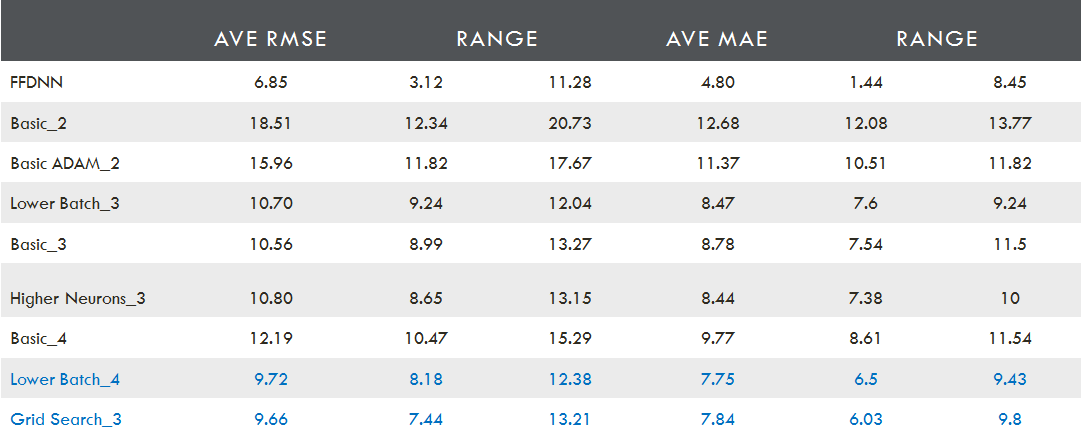
\includegraphics[width=\linewidth]{results.png}
         \caption{Prediction Results of each Models}
         \label{fig:results}
\end{figure}
\fi


\title{Predicting Lung Related Hospitalization in Davao City due to Air Quality via Recurrent Neural Networks}
\author{rjsperias}
\date{July 2018}
\begin{document}
\cleardoublepage
\begin{titlepage}
    \begin{center}
        
\includegraphics[width=1.5in]{addu.pdf}\\
        \vspace{1cm}
        \huge{Predicting Lung Related Hospitalization  in Davao City due to Air Quality via Recurrent Neural Networks}\\
        \vspace{1.5in}
        \large{Christian Owenn C. de Jesus}\\
        \large{Raphael John S. Perias}\\
        \vspace{1.5in}
        \large{ATENEO DE DAVAO UNIVERSITY\\SCHOOL OF ARTS AND SCIENCES\\DAVAO CITY}\\
        \vspace{1in}
        October 2018
    \end{center}
\end{titlepage}
\frontmatter
\chapter*{Abstract}
Air pollution is a growing concern in the developing world, and its presence is difficult to realize. Continuous exposure to pollution increases the risk of developing lung-related diseases.
However, due to the numerous factors affecting the development of disease, thorough statistical models have not been formulated that can reliably fit pollution concentration and change in hospitalizations from lung diseases. With the emergence of machine learning, more specifically Long Short-Term Memory (LSTM) based Recurrent Neural Networks (RNN), this study aims to develop a model that could reliably predict the changes in hospitalization based on the characteristics of an area and its pollution, taking into account the pollution present in previous days in a time-series. This model could then be used as a baseline for hospitals to distribute resources and overall be more efficient in administering aid to patients.
\tableofcontents{Table of Contents}
\mainmatter
\chapter{Introduction}
\section{Background of the Study}
    Increase in the concentration of air pollutants in various regions of the globe also increase the risk of death from lung complications. Due to the nature of air pollution, it is not easy to realize the presence and dangers of continued exposure. The human body can filter the air that is inhaled. However, it is not enough to remove all the risks from particles and pollutants ever present in the air.\cite{1971} Air pollutants are commonly not visible to the naked eye and could be small enough to penetrate conventional face masks. \cite{Shakya2016} Thus, without any visible indication, it becomes a factor for lung complications. \cite{2009} All lung complications have the symptoms of coughing and shortness of breath, which causes them to be dismissed as a simple cold or similar. Such is the case until the symptoms persist for several weeks and upon checkup, the person is diagnosed with severe diseases such as Pneumonia or Chronic bronchitis. Illustrating the risk from data collected by sensors could alert the person of what diseases he or she could contract from the polluted air.

    There are multiple studies that measured the pollution density in countries. There were also studies that took this pollution density and aligned it with the amount of hospitalized for lung-related diseases. These studies took note of environmental conditions and measured the trends in pollution for certain time periods. One such study was by Mansourian et al. (2011). However, data and numbers were the focus of these studies. The conclusion from observing the data was the presence of a statistically significant linear relationship between pollution density and number of hospitalized individuals. \cite{Mansourian2011}

    Other studies had organized previous data, while also including other factors such as age and previous lung complications, such as asthma. These studies had results trying to correlate risk factors and the actual risk of disease development. According to the study by Amadeo et al. (2015) children who have asthma who are continuously exposed to low concentration of pollution are found to have reduced lung function afterwards. However, a thorough statistical model has not been created due to the number of factors involved. \cite{Amadeo2015}

    More recently, from the development of machine learning techniques, algorithms have been made to relate risk factors with the percent risk of the onset of diseases. Although, these algorithms are currently applied to heart complications and post-organ transplant diseases. As the risk factors for these conditions are almost exclusively found within the body, for example, Body Fluid Analysis, Imaging, and Electric Pulse Measures. Thus, more data is compiled in a standard format, making the development of algorithms faster and easier.
    \section{Statement of the Problem}

    The study aims to develop a method to use data collected by sensors in real time to illustrate the correlation of hospitalization due to lung diseases and pollutants. Through a machine learning approach, the data will be aggregated and used to generate a model for prediction. This study also seeks to answer the following questions:
    \begin{enumerate}
        \item How to determine the concentration of pollutants in the air
        \item How to predict the number of lung-related hospitalizations due to poor air quality using RNN.
        \item How to demonstrate the accuracy of RNN model in predicting lung-related hospitalizations due to poor air quality.
    \end{enumerate}
    \section{Objectives}
    The study aims to develop a method to use data collected by sensors to illustrate the correlation of hospitalization due to lung diseases and pollutants and predict the changes based on the concentration of pollution. Additionally, it intends to accomplish the following objectives:
    \begin{enumerate}
        \item To explain the methods of determining the concentration of pollutants in the air
        \item To explain how to predict the number of lung-related hospitalizations due to poor air quality using RNN.
        \item To explain how to demonstrate the accuracy of RNN model in predicting lung-related hospitalizations due to poor air quality.
    \end{enumerate}
    \section{Significance of the Study}
    The results of the study could be used in health and air monitoring systems. The study could also be used for estimating the needed supplies by a hospital, should the change in hospitalization dramatically increase, institutions could be prepared, and treatments be administered much more efficiently.

    Additionally, it could be a starting point for future studies relating the multiple variables involved in lung health of individuals and or a population in an area. Should the focus be the algorithm, accuracy and speed could be improved, thus making a better implementation. On the other hand, it could give an insight on how each factor interacts with the human body and further studies on the effect of specific matter to the human body.
    \section{Scope and Limitations}
    The study utilizes local data sourced from institutions in Davao city which contain the relevant data and ignoring those which lack several factors. The study only estimated the total number of hospitalization from any lung disease and does not assume which specific disease it is, as it requires very specific data and situations. The study utilized an NVIDIA GTX 1060 6GB GPU for training the neural network from the lack of funds to apply for a cloud computing service.\\

    Hospitalization data was requested, and given by the following institutions, Department of Health, City Health Office Davao, Davao Medical School Foundation, and Davao Doctors Hospital. Unfortunately only the data received from Davao Doctors was usable, as other data were either very sparse or were recorded in different time intervals. In addition, the data acquired from Davao Doctors Hospital was recorded monthly, although daily and weekly data could be retrieved from
their system it would take a longer time. Initially, the data intervals of hospitalizations and pollution concentration should have been daily for maximum efficiency of the model, but due to lack of data from other approached hospitals and departments, the interval was changed to monthly.
\chapter{Review of Related Literature}
    \section{Air Pollutants and correlation to Health Exposure}
        \subsection{Particulate Matter}
        Particles are small objects that can be ascribed with properties such as volume or mass. It includes hazardous stuff such as dirt and soot, being one of the oldest air pollutants. They enter the atmosphere through natural or anthropogenic means \cite{knudsen2012particulate}. When particles become suspended in the air or atmosphere for long periods of time, they are now known as Particulate Matter, one of the common hazardous form of air pollutants.

        They can be classified as primary particles, which are particles that are directly emitted into the atmosphere or form by rapid condensation of gas molecules, or secondary particles which are formed from chemical transformation of existing gases (e.g. sulfur dioxide, nitrogen oxides, ammonia, etc.). \cite{finlayson2000chemistry}

        They are generally found in heavily urbanized areas, areas such as mines or factories that uses several chemicals, and even in homes. Studies stated by Rasmussen et al. in his work in 2012 show that 4 to 8\% percent of the total annual mortality rate are caused by air pollution due to PM alone in homes. PM2.5 and PM10 (2.5 and 10 denoting size in micrometers) are associated with cardiovascular and respiratory effects, respectively. Long-term exposure to PM2.5 have confirmed links with increasing risks of pneumonia \cite{Neupane2010} and exposure to PM10 has indeed have relations with increase mortality due to pneumonia and Chronic obstructive pulmonary disease (COPD), with mortality rates being modified depending on the overall characteristics of the city \cite{MedinaRamn2006}
        \subsection{Atmosphere-based Chemical Substances}
        Chemical-based substances also play a big role in air pollution and health risks. Besides the fact that some particulate matter, as mentioned, are formed from chemical gases, the latter themselves are already poisonous to humans. When it comes to the air, harmful substances such as nitrogen oxides, ozone, and sulfur dioxide come into play.

        In studies stated by Chauhan \& Johnston in their book in 2003, there is a 1.3\% increase in daily mortality rate with the increase of NO2 or O3 at 50 micrograms/m3. In addition, increased exposure of SO2 on asthmatic children led to increased respiratory symptoms, fever, and asthmatic medication. Furthermore, fine particles associated with the SO2 increased dyspnoea in children with mild asthma. \cite{doi:10.1093/bmb/ldg022}
        \subsection{Air Quality Index/Directive}
        The Air Quality Index/Directive (AQI/AQD) is a number used to summarize or describe the current pollution levels of the air or atmosphere. Each country has its own AQI, and each levels in the AQI denote different levels of air pollution and adverse health risks as stated by the Environmental Protection Agency (EPA) in their website. \cite{airbasics}
        \subsection{Low-cost Sensors}
        According to Nuria et al.
 (2016), current monitoring systems monitor air pollution concentration through measuring pollutants such as carbon monoxide, nitrogen oxide, and particulate matter (PM10 and PM2.5). Most of these sensors are very expensive in installing and maintaining; hence, they tested several commercial low-cost sensors (AQMesh v3.5) in their study.

        When measuring the concentration of several pollutants, the expanded uncertainty met the DQO criteria in the Air Quality Directive for some pollutants like NO, PM10, and PM2.5 while other pollutants like CO and NO2 showed expanded uncertainty exceeding the Data Quality Objectives’ (DQO) indicative methods. In short, the commercial low-cost sensors were deemed unsuitable; however, recent studies have shown that the application of field calibrations based on machine learning techniques can reduce the expanded uncertainty and improve overall performance. \cite{Castell2017}
    \section{Types of Recurring Neural Networks}
        \subsection{Long Short-Term Memory (LSTM)}
        Hochreiter and Schmidhuber [1997] invented Long Short-Term Memory networks, which are designed to solve the vanishing, and exploding gradient problem due to back-propagation when training artificial neural networks. Since then, it has been used in applications such as image processing and classification due to their ridiculous accuracy, and for their ability to store information over long-time intervals with minimal to no risk of it getting lost. \cite{Hochreiter:1997:LSM:1246443.1246450}

        A study by Zachary, et al. [2016] tested the efficiency of LSTM in diagnosing time series data gathered in the intensive care unit (ICU). While the networks were able to produce impressive results, there are some areas where LSTM performed worse due to the fact that some data progression does not follow with the standard linear progression commonly used in networks. \cite{DBLP:journals/corr/LiptonKEW15}
        \subsection{Gated Recurrent Unit (GRU)}
        GRUs are RNNs that functions mostly like LSTMs albeit with key differences, mainly that GRUs has fewer gates and that it is more efficient in sequence modeling and time series data analyzing when there are fewer parameters, and gathered data are used in short-time intervals (Britz, 2015). \cite{britz_2016}

        Zhengping et al. (2016) experimented on GRUs using multivariate series with missing values. The proponents wanted to exploit those missing values as a means to improve overall predicting performance in models; hence, the proponents created a new model called GRU-D, GRUs with decay mechanism that addresses the overall impact of missing values in the data in specific time intervals. The model itself proved valuable; it effectively handled the missing values in multivariate data through incorporating masking and time interval directly inside GRU architecture. Moreover, the model was able to make accurate early predictions before seeing all of the time series data, making it useful in fields such as healthcare. \cite{DBLP:journals/corr/ChePCSL16}
    \section{Other Machine Learning Approaches in Other Fields}
    Machine learning has been a definite staple in computer science, especially with the exploration and construction of algorithms. With risk estimation and prediction, machine learning has been proven to be useful in risk estimation, with its different methods being underutilized and can be further studied and can be further studied and polished. \cite{Kruppa2012} Other machine-learning approaches besides neural networks have also been used in other fields of risk estimation and prediction.
        \subsection{Artificial Neural Network}
        One study by Weng et al. (2017) tested four machine-learning approaches, neural networks included, against existing algorithms of cardiovascular risk prediction. The study proved that these machine-learning approaches significantly improved the overall performance of detecting individuals who will develop CVD and those that will not, with neural networks performing the best with predictive accuracy improved by 3.6\%. \cite{Weng2017}

        \subsection{Feedforward Neural Network}
        Studies by Jain et al. (2013) and Nasri (2010) showed that Artificial Neural Networks are not only good at predicting health risks but also managing risks in general. The ANNs used are of Feedforward (FFNN) type, which are neural networks that consist of nodes that don’t form a cycle; information goes in only one way (Hornik et al., 1988). Jain et al.’s model has an accuracy up to 90\% with a very low false positive rate (FPR) of 8.3\% at max. Nasri’s model has a much higher efficiency rate in risk management compared to fuzzy logic system and genetic algorithms. \cite{jain_singh_2013, nasri2010application}

        \subsection{Random Forest}
        A study by Gurm et al. (2014) created and analyzed a random forest-based risk model of receipt of transfusion in patients undergoing Percutaneous Coronary Intervention. The model, restricted based on Michigan, was indeed successful, albeit improvements can still be made. The model helped identify patient subgroups with a higher or lower risk of needing a transfusion, and it also proved PCI can be reliably estimated. \cite{Gurm2014}

        Another study by Ghatasheh (2014) used random forest trees to evaluate credit risk. Due to other approaches being black-boxed, random forest was suggested since it gives some insight on the dynamics and interactions between the underlying factors of credit risks. The results of the research show that random forest trees are a promising opportunity in Business Analytics, with pros like effective classification and accuracy being more beneficial to business domain experts. The findings also show how to improve decision trees in general through thorough investigation, testing and improving classification models. \cite{Ghatasheh2014BusinessAU}
        \subsection{Logistic Regression}
        Yanfeng et al. (2017) used logistic regression to create a risk model for pneumothorax after CT-guided needle biopsy and the different risk factors involved. Using univariate logistic regression analysis to determine risk factors, and then multivariate logistic regression analysis to break down which aforementioned risk factors are independent of each other, a regression analysis formula was formed to create the model. The model, integrated with all independent risk factors, predicted pneumothorax among patients with high accuracy. \cite{Zhao2017}
        \subsection{Gradient Boosting}
        Atkinson et al. (2013) used gradient boosting machine models (GBM) to assess whether it can improve bone fracture prediction. Gradient boosting “focuses on combining information from many variables that individually may not be significant but together are very informative.” Taking advantage of all the variables needed for the analysis, the GBM were able to differentiate fracture and non-fracture subjects with surprisingly high predictive ability.

        The study demonstrated that GBM has the potential to be very effective in its risk predicting in terms of the medical fields, precisely because of 3 reasons as stated by Atkinson et al.: (1) there is evidence that boosting methods are one of the approaches least affected by overfitting; (2) GBM models’ non-linearity and interactions between variables can be captured without prior specification; and (3) GBM incorporates the stochastic component, e.g. falling, that is so important in fracture pathogenesis. \cite{Atkinson2012}
    \section{Root-Mean-Square Error (RMSE)}
    The Root-Mean-Square Error is a statistical metric commonly used in measuring model performance. It is widely considered as the standard metric in model errors. As concluded by Chai et al. (2014) in their research, RMSE best represents model performance when error distribution is expected to be normal, and that it satisfies the triangle inequality requirement to be considered as a distance metric.
    
The formula, with respect to the estimated variable Xmodel is defined as the square root of the mean squared error (MSE) where Xobs is observed values and Xmodel is modeled values at time/place i.\\
    \begingroup
\Large
    \begin{math}
\centering
RMSE = \sqrt{}\frac{\sum_{n}^{i=1}\left ( X_{obs,i} - X_{model,i}\right )^{2}}{n}
\end{math}\\
\endgroup
    \section{Theoretical framework}
    \begin{figure} [ht]
        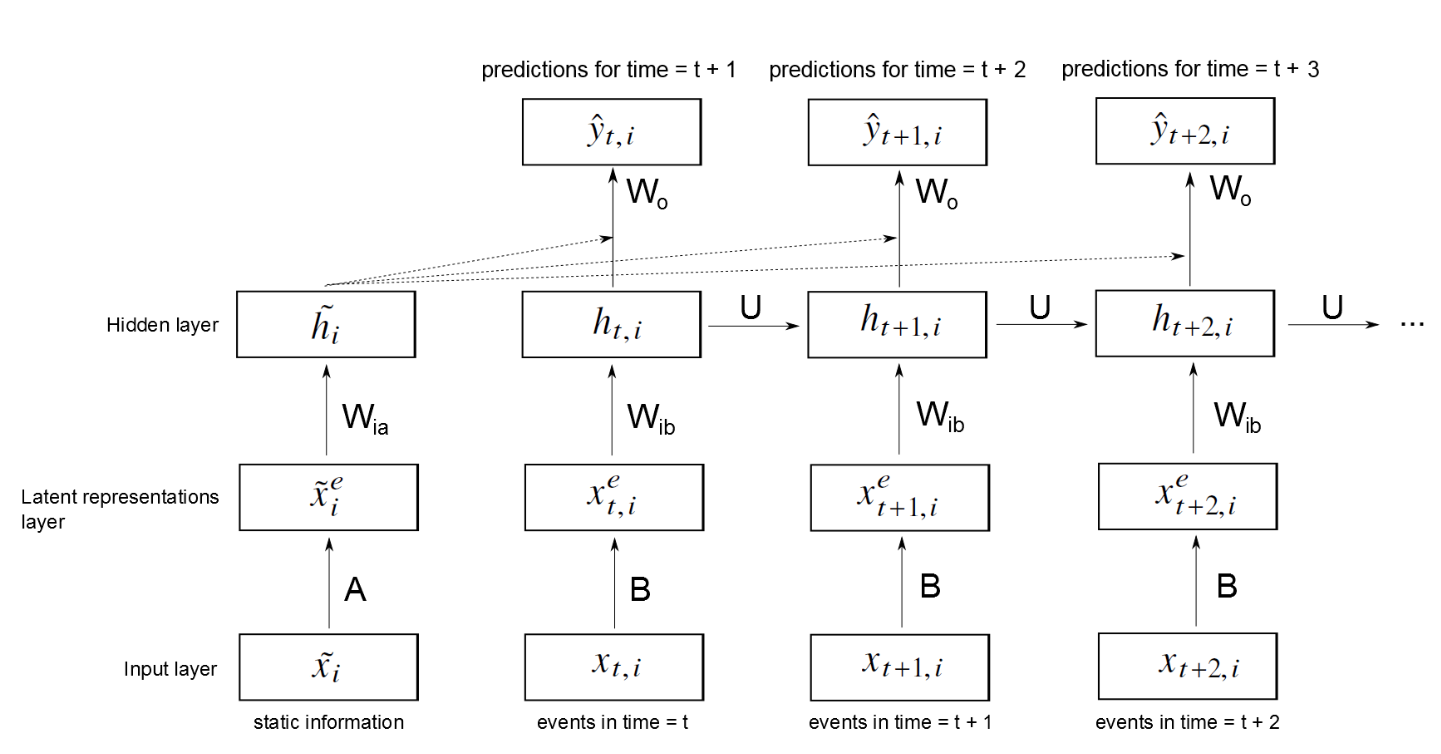
\includegraphics[width=6.5in]{rnnframework.png}
        \caption{RNN framework}
        \medskip
    \end{figure}
    A framework is created in the study conducted by Esteban, et al. wherein static and dynamic data of patients were used as predictors of future clinical events for several RNN implementations. It shows that the static information was first fed into an independent Feedforward Neural Network and the dynamic information into the RNN. Afterward, they then concatenated the hidden layers of both networks and provided the information into the output layer.

    As shown in the figure, the networks are fed latent representations of the data. The latent representations are computed by applying linear transformation on the raw input, which contains dynamic data and static data of the patient, except for the input for the independent network which only contains the static data of the patient. From the output of the network, a cost is calculated, the cost function applied was based on the Binary Cross Entropy function. \cite{DBLP:journals/corr/EstebanSYT16}
    \FloatBarrier
\chapter{Project Design and Methodology}
\section{Conceptual Framework}
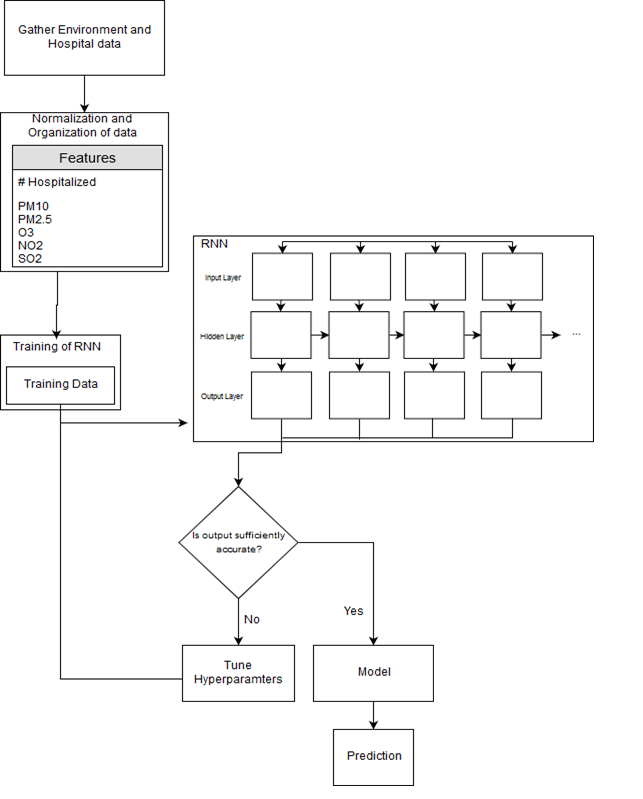
\includegraphics[height=6in]{conframework.png}
\section{Methodology}
    \subsection{Gathering of Pollution and Hospitalization Data}
    Two sets of data were then collected. The First set of data, labeled as Target, contains hospitalizations sourced from medical records of Davao Doctors Hospital. The hospitalizations listed patients who were diagnosed with lung diseases; specifically, Asthma, Chronic Obstructive Pulmonary Disease, Chronic Bronchitis, Emphysema, Lung Cancer, Pneumonia, and Tuberculosis. The second set of data, labeled as Features, contains pollution data sourced from the Department of Environment and Natural
    Resources(DENR). Pollution data was given by the DENR in several pdf files, each containing daily and weekly data for a year. The data contained the measurements collected by six monitoring stations, namely: DC Station 02, DC Station 07, DC Station 11, DC Station 14, DC Station 15, and DC Station 16, which were located at Amparo Subdivision Open Lot, Barangay Compound, Brgy 12-B, Davao Memorial Park, Phase II, Toril Open Park Area, Toril Poblacion, Davao City, Davao International Airport, AGL Open
Area, and Calinan National High School, Oval Open Area, respectively. The former four stations sample the air weekly while the latter two sample continuously daily. The pollution data used for training the models consist of the levels of concentrations of different pollutants that have been detected in different areas in Davao City; namely, PM10, NO2, O3, and SO2. All data gathered took place in 2015-2017, with a monthly interval. The data represented in a graph is shown below.\\
\begin{figure}[H]
\centering
\resizebox{!}{10cm}{%% Creator: Matplotlib, PGF backend
%%
%% To include the figure in your LaTeX document, write
%%   \input{<filename>.pgf}
%%
%% Make sure the required packages are loaded in your preamble
%%   \usepackage{pgf}
%%
%% Figures using additional raster images can only be included by \input if
%% they are in the same directory as the main LaTeX file. For loading figures
%% from other directories you can use the `import` package
%%   \usepackage{import}
%% and then include the figures with
%%   \import{<path to file>}{<filename>.pgf}
%%
%% Matplotlib used the following preamble
%%   \usepackage{fontspec}
%%   \setmainfont{Times New Roman}
%%   \setsansfont{Arial}
%%   \setmonofont{Courier New}
%%
\begingroup%
\makeatletter%
\begin{pgfpicture}%
\pgfpathrectangle{\pgfpointorigin}{\pgfqpoint{19.200000in}{9.930000in}}%
\pgfusepath{use as bounding box, clip}%
\begin{pgfscope}%
\pgfsetbuttcap%
\pgfsetmiterjoin%
\definecolor{currentfill}{rgb}{1.000000,1.000000,1.000000}%
\pgfsetfillcolor{currentfill}%
\pgfsetlinewidth{0.000000pt}%
\definecolor{currentstroke}{rgb}{1.000000,1.000000,1.000000}%
\pgfsetstrokecolor{currentstroke}%
\pgfsetdash{}{0pt}%
\pgfpathmoveto{\pgfqpoint{0.000000in}{0.000000in}}%
\pgfpathlineto{\pgfqpoint{19.200000in}{0.000000in}}%
\pgfpathlineto{\pgfqpoint{19.200000in}{9.930000in}}%
\pgfpathlineto{\pgfqpoint{0.000000in}{9.930000in}}%
\pgfpathclose%
\pgfusepath{fill}%
\end{pgfscope}%
\begin{pgfscope}%
\pgfsetbuttcap%
\pgfsetmiterjoin%
\definecolor{currentfill}{rgb}{0.917647,0.917647,0.949020}%
\pgfsetfillcolor{currentfill}%
\pgfsetlinewidth{0.000000pt}%
\definecolor{currentstroke}{rgb}{0.000000,0.000000,0.000000}%
\pgfsetstrokecolor{currentstroke}%
\pgfsetstrokeopacity{0.000000}%
\pgfsetdash{}{0pt}%
\pgfpathmoveto{\pgfqpoint{1.820000in}{1.022307in}}%
\pgfpathlineto{\pgfqpoint{17.367812in}{1.022307in}}%
\pgfpathlineto{\pgfqpoint{17.367812in}{9.619687in}}%
\pgfpathlineto{\pgfqpoint{1.820000in}{9.619687in}}%
\pgfpathclose%
\pgfusepath{fill}%
\end{pgfscope}%
\begin{pgfscope}%
\pgfpathrectangle{\pgfqpoint{1.820000in}{1.022307in}}{\pgfqpoint{15.547813in}{8.597380in}}%
\pgfusepath{clip}%
\pgfsetroundcap%
\pgfsetroundjoin%
\pgfsetlinewidth{0.803000pt}%
\definecolor{currentstroke}{rgb}{1.000000,1.000000,1.000000}%
\pgfsetstrokecolor{currentstroke}%
\pgfsetdash{}{0pt}%
\pgfpathmoveto{\pgfqpoint{2.526719in}{1.022307in}}%
\pgfpathlineto{\pgfqpoint{2.526719in}{9.619687in}}%
\pgfusepath{stroke}%
\end{pgfscope}%
\begin{pgfscope}%
\definecolor{textcolor}{rgb}{0.150000,0.150000,0.150000}%
\pgfsetstrokecolor{textcolor}%
\pgfsetfillcolor{textcolor}%
\pgftext[x=2.526719in,y=0.973696in,,top]{\color{textcolor}\sffamily\fontsize{10.000000}{12.000000}\selectfont 0}%
\end{pgfscope}%
\begin{pgfscope}%
\pgfpathrectangle{\pgfqpoint{1.820000in}{1.022307in}}{\pgfqpoint{15.547813in}{8.597380in}}%
\pgfusepath{clip}%
\pgfsetroundcap%
\pgfsetroundjoin%
\pgfsetlinewidth{0.803000pt}%
\definecolor{currentstroke}{rgb}{1.000000,1.000000,1.000000}%
\pgfsetstrokecolor{currentstroke}%
\pgfsetdash{}{0pt}%
\pgfpathmoveto{\pgfqpoint{5.298165in}{1.022307in}}%
\pgfpathlineto{\pgfqpoint{5.298165in}{9.619687in}}%
\pgfusepath{stroke}%
\end{pgfscope}%
\begin{pgfscope}%
\definecolor{textcolor}{rgb}{0.150000,0.150000,0.150000}%
\pgfsetstrokecolor{textcolor}%
\pgfsetfillcolor{textcolor}%
\pgftext[x=5.298165in,y=0.973696in,,top]{\color{textcolor}\sffamily\fontsize{10.000000}{12.000000}\selectfont 20}%
\end{pgfscope}%
\begin{pgfscope}%
\pgfpathrectangle{\pgfqpoint{1.820000in}{1.022307in}}{\pgfqpoint{15.547813in}{8.597380in}}%
\pgfusepath{clip}%
\pgfsetroundcap%
\pgfsetroundjoin%
\pgfsetlinewidth{0.803000pt}%
\definecolor{currentstroke}{rgb}{1.000000,1.000000,1.000000}%
\pgfsetstrokecolor{currentstroke}%
\pgfsetdash{}{0pt}%
\pgfpathmoveto{\pgfqpoint{8.069611in}{1.022307in}}%
\pgfpathlineto{\pgfqpoint{8.069611in}{9.619687in}}%
\pgfusepath{stroke}%
\end{pgfscope}%
\begin{pgfscope}%
\definecolor{textcolor}{rgb}{0.150000,0.150000,0.150000}%
\pgfsetstrokecolor{textcolor}%
\pgfsetfillcolor{textcolor}%
\pgftext[x=8.069611in,y=0.973696in,,top]{\color{textcolor}\sffamily\fontsize{10.000000}{12.000000}\selectfont 40}%
\end{pgfscope}%
\begin{pgfscope}%
\pgfpathrectangle{\pgfqpoint{1.820000in}{1.022307in}}{\pgfqpoint{15.547813in}{8.597380in}}%
\pgfusepath{clip}%
\pgfsetroundcap%
\pgfsetroundjoin%
\pgfsetlinewidth{0.803000pt}%
\definecolor{currentstroke}{rgb}{1.000000,1.000000,1.000000}%
\pgfsetstrokecolor{currentstroke}%
\pgfsetdash{}{0pt}%
\pgfpathmoveto{\pgfqpoint{10.841057in}{1.022307in}}%
\pgfpathlineto{\pgfqpoint{10.841057in}{9.619687in}}%
\pgfusepath{stroke}%
\end{pgfscope}%
\begin{pgfscope}%
\definecolor{textcolor}{rgb}{0.150000,0.150000,0.150000}%
\pgfsetstrokecolor{textcolor}%
\pgfsetfillcolor{textcolor}%
\pgftext[x=10.841057in,y=0.973696in,,top]{\color{textcolor}\sffamily\fontsize{10.000000}{12.000000}\selectfont 60}%
\end{pgfscope}%
\begin{pgfscope}%
\pgfpathrectangle{\pgfqpoint{1.820000in}{1.022307in}}{\pgfqpoint{15.547813in}{8.597380in}}%
\pgfusepath{clip}%
\pgfsetroundcap%
\pgfsetroundjoin%
\pgfsetlinewidth{0.803000pt}%
\definecolor{currentstroke}{rgb}{1.000000,1.000000,1.000000}%
\pgfsetstrokecolor{currentstroke}%
\pgfsetdash{}{0pt}%
\pgfpathmoveto{\pgfqpoint{13.612503in}{1.022307in}}%
\pgfpathlineto{\pgfqpoint{13.612503in}{9.619687in}}%
\pgfusepath{stroke}%
\end{pgfscope}%
\begin{pgfscope}%
\definecolor{textcolor}{rgb}{0.150000,0.150000,0.150000}%
\pgfsetstrokecolor{textcolor}%
\pgfsetfillcolor{textcolor}%
\pgftext[x=13.612503in,y=0.973696in,,top]{\color{textcolor}\sffamily\fontsize{10.000000}{12.000000}\selectfont 80}%
\end{pgfscope}%
\begin{pgfscope}%
\pgfpathrectangle{\pgfqpoint{1.820000in}{1.022307in}}{\pgfqpoint{15.547813in}{8.597380in}}%
\pgfusepath{clip}%
\pgfsetroundcap%
\pgfsetroundjoin%
\pgfsetlinewidth{0.803000pt}%
\definecolor{currentstroke}{rgb}{1.000000,1.000000,1.000000}%
\pgfsetstrokecolor{currentstroke}%
\pgfsetdash{}{0pt}%
\pgfpathmoveto{\pgfqpoint{16.383949in}{1.022307in}}%
\pgfpathlineto{\pgfqpoint{16.383949in}{9.619687in}}%
\pgfusepath{stroke}%
\end{pgfscope}%
\begin{pgfscope}%
\definecolor{textcolor}{rgb}{0.150000,0.150000,0.150000}%
\pgfsetstrokecolor{textcolor}%
\pgfsetfillcolor{textcolor}%
\pgftext[x=16.383949in,y=0.973696in,,top]{\color{textcolor}\sffamily\fontsize{10.000000}{12.000000}\selectfont 100}%
\end{pgfscope}%
\begin{pgfscope}%
\definecolor{textcolor}{rgb}{0.150000,0.150000,0.150000}%
\pgfsetstrokecolor{textcolor}%
\pgfsetfillcolor{textcolor}%
\pgftext[x=9.593906in,y=0.791120in,,top]{\color{textcolor}\sffamily\fontsize{10.000000}{12.000000}\selectfont day}%
\end{pgfscope}%
\begin{pgfscope}%
\pgfpathrectangle{\pgfqpoint{1.820000in}{1.022307in}}{\pgfqpoint{15.547813in}{8.597380in}}%
\pgfusepath{clip}%
\pgfsetroundcap%
\pgfsetroundjoin%
\pgfsetlinewidth{0.803000pt}%
\definecolor{currentstroke}{rgb}{1.000000,1.000000,1.000000}%
\pgfsetstrokecolor{currentstroke}%
\pgfsetdash{}{0pt}%
\pgfpathmoveto{\pgfqpoint{1.820000in}{1.131824in}}%
\pgfpathlineto{\pgfqpoint{17.367812in}{1.131824in}}%
\pgfusepath{stroke}%
\end{pgfscope}%
\begin{pgfscope}%
\definecolor{textcolor}{rgb}{0.150000,0.150000,0.150000}%
\pgfsetstrokecolor{textcolor}%
\pgfsetfillcolor{textcolor}%
\pgftext[x=1.694146in,y=1.082114in,left,base]{\color{textcolor}\sffamily\fontsize{10.000000}{12.000000}\selectfont 0}%
\end{pgfscope}%
\begin{pgfscope}%
\pgfpathrectangle{\pgfqpoint{1.820000in}{1.022307in}}{\pgfqpoint{15.547813in}{8.597380in}}%
\pgfusepath{clip}%
\pgfsetroundcap%
\pgfsetroundjoin%
\pgfsetlinewidth{0.803000pt}%
\definecolor{currentstroke}{rgb}{1.000000,1.000000,1.000000}%
\pgfsetstrokecolor{currentstroke}%
\pgfsetdash{}{0pt}%
\pgfpathmoveto{\pgfqpoint{1.820000in}{2.419117in}}%
\pgfpathlineto{\pgfqpoint{17.367812in}{2.419117in}}%
\pgfusepath{stroke}%
\end{pgfscope}%
\begin{pgfscope}%
\definecolor{textcolor}{rgb}{0.150000,0.150000,0.150000}%
\pgfsetstrokecolor{textcolor}%
\pgfsetfillcolor{textcolor}%
\pgftext[x=1.616902in,y=2.369407in,left,base]{\color{textcolor}\sffamily\fontsize{10.000000}{12.000000}\selectfont 20}%
\end{pgfscope}%
\begin{pgfscope}%
\pgfpathrectangle{\pgfqpoint{1.820000in}{1.022307in}}{\pgfqpoint{15.547813in}{8.597380in}}%
\pgfusepath{clip}%
\pgfsetroundcap%
\pgfsetroundjoin%
\pgfsetlinewidth{0.803000pt}%
\definecolor{currentstroke}{rgb}{1.000000,1.000000,1.000000}%
\pgfsetstrokecolor{currentstroke}%
\pgfsetdash{}{0pt}%
\pgfpathmoveto{\pgfqpoint{1.820000in}{3.706410in}}%
\pgfpathlineto{\pgfqpoint{17.367812in}{3.706410in}}%
\pgfusepath{stroke}%
\end{pgfscope}%
\begin{pgfscope}%
\definecolor{textcolor}{rgb}{0.150000,0.150000,0.150000}%
\pgfsetstrokecolor{textcolor}%
\pgfsetfillcolor{textcolor}%
\pgftext[x=1.616902in,y=3.656700in,left,base]{\color{textcolor}\sffamily\fontsize{10.000000}{12.000000}\selectfont 40}%
\end{pgfscope}%
\begin{pgfscope}%
\pgfpathrectangle{\pgfqpoint{1.820000in}{1.022307in}}{\pgfqpoint{15.547813in}{8.597380in}}%
\pgfusepath{clip}%
\pgfsetroundcap%
\pgfsetroundjoin%
\pgfsetlinewidth{0.803000pt}%
\definecolor{currentstroke}{rgb}{1.000000,1.000000,1.000000}%
\pgfsetstrokecolor{currentstroke}%
\pgfsetdash{}{0pt}%
\pgfpathmoveto{\pgfqpoint{1.820000in}{4.993703in}}%
\pgfpathlineto{\pgfqpoint{17.367812in}{4.993703in}}%
\pgfusepath{stroke}%
\end{pgfscope}%
\begin{pgfscope}%
\definecolor{textcolor}{rgb}{0.150000,0.150000,0.150000}%
\pgfsetstrokecolor{textcolor}%
\pgfsetfillcolor{textcolor}%
\pgftext[x=1.616902in,y=4.943993in,left,base]{\color{textcolor}\sffamily\fontsize{10.000000}{12.000000}\selectfont 60}%
\end{pgfscope}%
\begin{pgfscope}%
\pgfpathrectangle{\pgfqpoint{1.820000in}{1.022307in}}{\pgfqpoint{15.547813in}{8.597380in}}%
\pgfusepath{clip}%
\pgfsetroundcap%
\pgfsetroundjoin%
\pgfsetlinewidth{0.803000pt}%
\definecolor{currentstroke}{rgb}{1.000000,1.000000,1.000000}%
\pgfsetstrokecolor{currentstroke}%
\pgfsetdash{}{0pt}%
\pgfpathmoveto{\pgfqpoint{1.820000in}{6.280996in}}%
\pgfpathlineto{\pgfqpoint{17.367812in}{6.280996in}}%
\pgfusepath{stroke}%
\end{pgfscope}%
\begin{pgfscope}%
\definecolor{textcolor}{rgb}{0.150000,0.150000,0.150000}%
\pgfsetstrokecolor{textcolor}%
\pgfsetfillcolor{textcolor}%
\pgftext[x=1.616902in,y=6.231287in,left,base]{\color{textcolor}\sffamily\fontsize{10.000000}{12.000000}\selectfont 80}%
\end{pgfscope}%
\begin{pgfscope}%
\pgfpathrectangle{\pgfqpoint{1.820000in}{1.022307in}}{\pgfqpoint{15.547813in}{8.597380in}}%
\pgfusepath{clip}%
\pgfsetroundcap%
\pgfsetroundjoin%
\pgfsetlinewidth{0.803000pt}%
\definecolor{currentstroke}{rgb}{1.000000,1.000000,1.000000}%
\pgfsetstrokecolor{currentstroke}%
\pgfsetdash{}{0pt}%
\pgfpathmoveto{\pgfqpoint{1.820000in}{7.568289in}}%
\pgfpathlineto{\pgfqpoint{17.367812in}{7.568289in}}%
\pgfusepath{stroke}%
\end{pgfscope}%
\begin{pgfscope}%
\definecolor{textcolor}{rgb}{0.150000,0.150000,0.150000}%
\pgfsetstrokecolor{textcolor}%
\pgfsetfillcolor{textcolor}%
\pgftext[x=1.539659in,y=7.518580in,left,base]{\color{textcolor}\sffamily\fontsize{10.000000}{12.000000}\selectfont 100}%
\end{pgfscope}%
\begin{pgfscope}%
\pgfpathrectangle{\pgfqpoint{1.820000in}{1.022307in}}{\pgfqpoint{15.547813in}{8.597380in}}%
\pgfusepath{clip}%
\pgfsetroundcap%
\pgfsetroundjoin%
\pgfsetlinewidth{0.803000pt}%
\definecolor{currentstroke}{rgb}{1.000000,1.000000,1.000000}%
\pgfsetstrokecolor{currentstroke}%
\pgfsetdash{}{0pt}%
\pgfpathmoveto{\pgfqpoint{1.820000in}{8.855582in}}%
\pgfpathlineto{\pgfqpoint{17.367812in}{8.855582in}}%
\pgfusepath{stroke}%
\end{pgfscope}%
\begin{pgfscope}%
\definecolor{textcolor}{rgb}{0.150000,0.150000,0.150000}%
\pgfsetstrokecolor{textcolor}%
\pgfsetfillcolor{textcolor}%
\pgftext[x=1.539659in,y=8.805873in,left,base]{\color{textcolor}\sffamily\fontsize{10.000000}{12.000000}\selectfont 120}%
\end{pgfscope}%
\begin{pgfscope}%
\definecolor{textcolor}{rgb}{0.150000,0.150000,0.150000}%
\pgfsetstrokecolor{textcolor}%
\pgfsetfillcolor{textcolor}%
\pgftext[x=1.484103in,y=5.320997in,,bottom,rotate=90.000000]{\color{textcolor}\sffamily\fontsize{10.000000}{12.000000}\selectfont µg/Ncm}%
\end{pgfscope}%
\begin{pgfscope}%
\pgfpathrectangle{\pgfqpoint{1.820000in}{1.022307in}}{\pgfqpoint{15.547813in}{8.597380in}}%
\pgfusepath{clip}%
\pgfsetroundcap%
\pgfsetroundjoin%
\pgfsetlinewidth{1.505625pt}%
\definecolor{currentstroke}{rgb}{0.121569,0.466667,0.705882}%
\pgfsetstrokecolor{currentstroke}%
\pgfsetdash{}{0pt}%
\pgfpathmoveto{\pgfqpoint{2.526719in}{3.358841in}}%
\pgfpathlineto{\pgfqpoint{2.665291in}{2.824614in}}%
\pgfpathlineto{\pgfqpoint{2.803863in}{3.204366in}}%
\pgfpathlineto{\pgfqpoint{2.942436in}{4.324311in}}%
\pgfpathlineto{\pgfqpoint{3.081008in}{3.500443in}}%
\pgfpathlineto{\pgfqpoint{3.219580in}{2.534973in}}%
\pgfpathlineto{\pgfqpoint{3.358153in}{5.572985in}}%
\pgfpathlineto{\pgfqpoint{3.496725in}{4.742681in}}%
\pgfpathlineto{\pgfqpoint{3.635297in}{3.738592in}}%
\pgfpathlineto{\pgfqpoint{3.773869in}{3.777211in}}%
\pgfpathmoveto{\pgfqpoint{4.051014in}{3.094946in}}%
\pgfpathlineto{\pgfqpoint{4.189586in}{3.403896in}}%
\pgfpathlineto{\pgfqpoint{4.328159in}{3.654918in}}%
\pgfpathmoveto{\pgfqpoint{4.605303in}{3.056327in}}%
\pgfpathlineto{\pgfqpoint{4.743876in}{3.860885in}}%
\pgfpathlineto{\pgfqpoint{4.882448in}{3.577681in}}%
\pgfpathlineto{\pgfqpoint{5.021020in}{2.901852in}}%
\pgfpathlineto{\pgfqpoint{5.159593in}{2.805305in}}%
\pgfpathlineto{\pgfqpoint{5.298165in}{2.740940in}}%
\pgfpathlineto{\pgfqpoint{5.436737in}{3.056327in}}%
\pgfpathlineto{\pgfqpoint{5.575309in}{2.277515in}}%
\pgfpathlineto{\pgfqpoint{5.713882in}{4.144090in}}%
\pgfpathlineto{\pgfqpoint{5.852454in}{4.601079in}}%
\pgfpathlineto{\pgfqpoint{5.991026in}{3.037018in}}%
\pgfpathlineto{\pgfqpoint{6.129599in}{3.352404in}}%
\pgfusepath{stroke}%
\end{pgfscope}%
\begin{pgfscope}%
\pgfpathrectangle{\pgfqpoint{1.820000in}{1.022307in}}{\pgfqpoint{15.547813in}{8.597380in}}%
\pgfusepath{clip}%
\pgfsetroundcap%
\pgfsetroundjoin%
\pgfsetlinewidth{1.505625pt}%
\definecolor{currentstroke}{rgb}{1.000000,0.498039,0.054902}%
\pgfsetstrokecolor{currentstroke}%
\pgfsetdash{}{0pt}%
\pgfpathmoveto{\pgfqpoint{2.665291in}{3.526189in}}%
\pgfpathlineto{\pgfqpoint{2.803863in}{4.671880in}}%
\pgfpathlineto{\pgfqpoint{2.942436in}{4.691189in}}%
\pgfpathlineto{\pgfqpoint{3.081008in}{4.182708in}}%
\pgfpathlineto{\pgfqpoint{3.219580in}{3.854449in}}%
\pgfpathlineto{\pgfqpoint{3.358153in}{3.609863in}}%
\pgfpathlineto{\pgfqpoint{3.496725in}{5.025885in}}%
\pgfpathlineto{\pgfqpoint{3.635297in}{5.901245in}}%
\pgfpathlineto{\pgfqpoint{3.773869in}{6.422598in}}%
\pgfpathlineto{\pgfqpoint{3.912442in}{3.082073in}}%
\pgfpathlineto{\pgfqpoint{4.051014in}{3.448951in}}%
\pgfpathlineto{\pgfqpoint{4.189586in}{3.397460in}}%
\pgfpathlineto{\pgfqpoint{4.328159in}{4.562460in}}%
\pgfpathlineto{\pgfqpoint{4.466731in}{3.120692in}}%
\pgfpathlineto{\pgfqpoint{4.605303in}{3.204366in}}%
\pgfpathlineto{\pgfqpoint{4.743876in}{3.616299in}}%
\pgfpathlineto{\pgfqpoint{4.882448in}{3.255857in}}%
\pgfpathlineto{\pgfqpoint{5.021020in}{3.539062in}}%
\pgfpathlineto{\pgfqpoint{5.159593in}{3.545498in}}%
\pgfpathlineto{\pgfqpoint{5.298165in}{3.802957in}}%
\pgfpathlineto{\pgfqpoint{5.436737in}{3.822266in}}%
\pgfpathlineto{\pgfqpoint{5.575309in}{4.620388in}}%
\pgfpathlineto{\pgfqpoint{5.713882in}{6.596383in}}%
\pgfusepath{stroke}%
\end{pgfscope}%
\begin{pgfscope}%
\pgfpathrectangle{\pgfqpoint{1.820000in}{1.022307in}}{\pgfqpoint{15.547813in}{8.597380in}}%
\pgfusepath{clip}%
\pgfsetroundcap%
\pgfsetroundjoin%
\pgfsetlinewidth{1.505625pt}%
\definecolor{currentstroke}{rgb}{0.172549,0.627451,0.172549}%
\pgfsetstrokecolor{currentstroke}%
\pgfsetdash{}{0pt}%
\pgfpathmoveto{\pgfqpoint{4.051014in}{2.483482in}}%
\pgfpathlineto{\pgfqpoint{4.189586in}{3.140001in}}%
\pgfpathlineto{\pgfqpoint{4.328159in}{2.773122in}}%
\pgfpathlineto{\pgfqpoint{4.466731in}{2.805305in}}%
\pgfpathlineto{\pgfqpoint{4.605303in}{3.365277in}}%
\pgfpathlineto{\pgfqpoint{4.743876in}{3.468261in}}%
\pgfpathlineto{\pgfqpoint{4.882448in}{2.477045in}}%
\pgfpathlineto{\pgfqpoint{5.021020in}{3.062763in}}%
\pgfpathlineto{\pgfqpoint{5.159593in}{2.399807in}}%
\pgfpathlineto{\pgfqpoint{5.298165in}{2.438426in}}%
\pgfpathlineto{\pgfqpoint{5.436737in}{4.807046in}}%
\pgfpathlineto{\pgfqpoint{5.575309in}{2.071548in}}%
\pgfpathlineto{\pgfqpoint{5.713882in}{7.400941in}}%
\pgfpathmoveto{\pgfqpoint{5.991026in}{2.612211in}}%
\pgfpathlineto{\pgfqpoint{6.129599in}{2.412680in}}%
\pgfpathlineto{\pgfqpoint{6.268171in}{6.004228in}}%
\pgfpathlineto{\pgfqpoint{6.406743in}{3.867322in}}%
\pgfpathlineto{\pgfqpoint{6.545316in}{3.860885in}}%
\pgfpathlineto{\pgfqpoint{6.683888in}{3.867322in}}%
\pgfpathlineto{\pgfqpoint{6.822460in}{3.468261in}}%
\pgfpathlineto{\pgfqpoint{6.961032in}{2.972653in}}%
\pgfpathlineto{\pgfqpoint{7.099605in}{4.691189in}}%
\pgfpathlineto{\pgfqpoint{7.238177in}{3.802957in}}%
\pgfpathlineto{\pgfqpoint{7.376749in}{7.336577in}}%
\pgfpathlineto{\pgfqpoint{7.515322in}{4.710499in}}%
\pgfpathlineto{\pgfqpoint{7.653894in}{3.436078in}}%
\pgfpathlineto{\pgfqpoint{7.792466in}{4.118344in}}%
\pgfpathlineto{\pgfqpoint{7.931039in}{6.377543in}}%
\pgfpathlineto{\pgfqpoint{8.069611in}{3.075636in}}%
\pgfpathlineto{\pgfqpoint{8.208183in}{4.279255in}}%
\pgfpathlineto{\pgfqpoint{8.346756in}{2.882542in}}%
\pgfpathlineto{\pgfqpoint{8.485328in}{2.496354in}}%
\pgfpathlineto{\pgfqpoint{8.623900in}{2.702321in}}%
\pgfpathlineto{\pgfqpoint{8.762472in}{2.444863in}}%
\pgfpathlineto{\pgfqpoint{8.901045in}{2.843924in}}%
\pgfpathlineto{\pgfqpoint{9.039617in}{3.732156in}}%
\pgfpathlineto{\pgfqpoint{9.178189in}{2.882542in}}%
\pgfpathmoveto{\pgfqpoint{9.455334in}{4.083587in}}%
\pgfpathlineto{\pgfqpoint{9.593906in}{3.622092in}}%
\pgfpathlineto{\pgfqpoint{9.732479in}{3.228181in}}%
\pgfpathlineto{\pgfqpoint{9.871051in}{2.656622in}}%
\pgfpathlineto{\pgfqpoint{10.009623in}{3.447664in}}%
\pgfpathlineto{\pgfqpoint{10.148195in}{2.567799in}}%
\pgfpathlineto{\pgfqpoint{10.286768in}{3.052465in}}%
\pgfpathlineto{\pgfqpoint{10.425340in}{3.789440in}}%
\pgfpathlineto{\pgfqpoint{10.563912in}{2.762180in}}%
\pgfpathlineto{\pgfqpoint{10.702485in}{3.094946in}}%
\pgfpathlineto{\pgfqpoint{10.841057in}{3.205653in}}%
\pgfpathlineto{\pgfqpoint{10.979629in}{2.394658in}}%
\pgfpathlineto{\pgfqpoint{11.118202in}{2.899277in}}%
\pgfpathlineto{\pgfqpoint{11.256774in}{3.016421in}}%
\pgfpathlineto{\pgfqpoint{11.395346in}{3.004835in}}%
\pgfpathlineto{\pgfqpoint{11.533919in}{1.413097in}}%
\pgfpathlineto{\pgfqpoint{11.672491in}{2.032929in}}%
\pgfpathlineto{\pgfqpoint{11.811063in}{4.216822in}}%
\pgfpathlineto{\pgfqpoint{11.949635in}{3.038305in}}%
\pgfpathlineto{\pgfqpoint{12.088208in}{3.656206in}}%
\pgfpathlineto{\pgfqpoint{12.226780in}{3.319578in}}%
\pgfpathlineto{\pgfqpoint{12.365352in}{2.814316in}}%
\pgfpathlineto{\pgfqpoint{12.503925in}{4.776794in}}%
\pgfpathlineto{\pgfqpoint{12.642497in}{3.359485in}}%
\pgfpathlineto{\pgfqpoint{12.781069in}{3.389092in}}%
\pgfpathlineto{\pgfqpoint{12.919642in}{3.927824in}}%
\pgfpathlineto{\pgfqpoint{13.058214in}{2.375349in}}%
\pgfpathlineto{\pgfqpoint{13.196786in}{4.259302in}}%
\pgfpathlineto{\pgfqpoint{13.335358in}{2.627658in}}%
\pgfpathlineto{\pgfqpoint{13.473931in}{4.149882in}}%
\pgfpathlineto{\pgfqpoint{13.612503in}{3.801670in}}%
\pgfpathlineto{\pgfqpoint{13.751075in}{2.623153in}}%
\pgfpathlineto{\pgfqpoint{13.889648in}{4.601722in}}%
\pgfpathlineto{\pgfqpoint{14.028220in}{3.793946in}}%
\pgfpathlineto{\pgfqpoint{14.166792in}{4.114482in}}%
\pgfpathlineto{\pgfqpoint{14.305365in}{4.583057in}}%
\pgfpathlineto{\pgfqpoint{14.443937in}{4.157606in}}%
\pgfpathlineto{\pgfqpoint{14.582509in}{3.130990in}}%
\pgfpathlineto{\pgfqpoint{14.721081in}{3.848012in}}%
\pgfpathmoveto{\pgfqpoint{14.998226in}{4.005706in}}%
\pgfpathlineto{\pgfqpoint{15.136798in}{3.328589in}}%
\pgfpathlineto{\pgfqpoint{15.275371in}{3.185700in}}%
\pgfpathlineto{\pgfqpoint{15.413943in}{5.147535in}}%
\pgfpathlineto{\pgfqpoint{15.552515in}{2.913437in}}%
\pgfpathlineto{\pgfqpoint{15.691088in}{6.392991in}}%
\pgfpathlineto{\pgfqpoint{15.829660in}{2.513733in}}%
\pgfpathlineto{\pgfqpoint{15.968232in}{5.593582in}}%
\pgfpathlineto{\pgfqpoint{16.106805in}{2.319352in}}%
\pgfpathlineto{\pgfqpoint{16.245377in}{3.085935in}}%
\pgfpathlineto{\pgfqpoint{16.383949in}{3.594415in}}%
\pgfpathlineto{\pgfqpoint{16.522521in}{4.241924in}}%
\pgfpathlineto{\pgfqpoint{16.661094in}{4.073932in}}%
\pgfusepath{stroke}%
\end{pgfscope}%
\begin{pgfscope}%
\pgfpathrectangle{\pgfqpoint{1.820000in}{1.022307in}}{\pgfqpoint{15.547813in}{8.597380in}}%
\pgfusepath{clip}%
\pgfsetroundcap%
\pgfsetroundjoin%
\pgfsetlinewidth{1.505625pt}%
\definecolor{currentstroke}{rgb}{0.839216,0.152941,0.156863}%
\pgfsetstrokecolor{currentstroke}%
\pgfsetdash{}{0pt}%
\pgfpathmoveto{\pgfqpoint{3.912442in}{2.528537in}}%
\pgfpathlineto{\pgfqpoint{4.051014in}{5.103123in}}%
\pgfpathlineto{\pgfqpoint{4.189586in}{5.566549in}}%
\pgfpathlineto{\pgfqpoint{4.328159in}{5.328399in}}%
\pgfpathlineto{\pgfqpoint{4.466731in}{3.905940in}}%
\pgfpathlineto{\pgfqpoint{4.605303in}{6.280996in}}%
\pgfpathlineto{\pgfqpoint{4.743876in}{5.836880in}}%
\pgfpathlineto{\pgfqpoint{4.882448in}{4.929338in}}%
\pgfpathmoveto{\pgfqpoint{5.159593in}{4.195581in}}%
\pgfpathlineto{\pgfqpoint{5.298165in}{4.543151in}}%
\pgfpathlineto{\pgfqpoint{5.436737in}{3.706410in}}%
\pgfpathlineto{\pgfqpoint{5.575309in}{1.936382in}}%
\pgfpathlineto{\pgfqpoint{5.713882in}{9.125914in}}%
\pgfpathlineto{\pgfqpoint{5.852454in}{3.030581in}}%
\pgfpathmoveto{\pgfqpoint{6.268171in}{5.045195in}}%
\pgfpathlineto{\pgfqpoint{6.406743in}{4.105471in}}%
\pgfpathlineto{\pgfqpoint{6.545316in}{4.118344in}}%
\pgfpathlineto{\pgfqpoint{6.683888in}{6.094339in}}%
\pgfpathlineto{\pgfqpoint{6.822460in}{5.572985in}}%
\pgfpathlineto{\pgfqpoint{6.961032in}{6.544891in}}%
\pgfpathlineto{\pgfqpoint{7.099605in}{4.890720in}}%
\pgfpathlineto{\pgfqpoint{7.238177in}{6.480527in}}%
\pgfpathlineto{\pgfqpoint{7.376749in}{8.855582in}}%
\pgfpathlineto{\pgfqpoint{7.515322in}{9.228897in}}%
\pgfpathlineto{\pgfqpoint{7.653894in}{6.667184in}}%
\pgfpathlineto{\pgfqpoint{7.792466in}{3.867322in}}%
\pgfpathlineto{\pgfqpoint{7.931039in}{7.780693in}}%
\pgfpathlineto{\pgfqpoint{8.069611in}{5.862626in}}%
\pgfpathlineto{\pgfqpoint{8.208183in}{2.258205in}}%
\pgfpathlineto{\pgfqpoint{8.346756in}{4.472349in}}%
\pgfpathlineto{\pgfqpoint{8.485328in}{4.227764in}}%
\pgfpathlineto{\pgfqpoint{8.623900in}{5.444256in}}%
\pgfpathlineto{\pgfqpoint{8.762472in}{4.465913in}}%
\pgfpathlineto{\pgfqpoint{8.901045in}{5.470002in}}%
\pgfpathlineto{\pgfqpoint{9.039617in}{3.957432in}}%
\pgfpathlineto{\pgfqpoint{9.178189in}{4.807046in}}%
\pgfpathlineto{\pgfqpoint{9.316762in}{6.187667in}}%
\pgfpathlineto{\pgfqpoint{9.455334in}{3.738592in}}%
\pgfpathlineto{\pgfqpoint{9.593906in}{4.367435in}}%
\pgfpathlineto{\pgfqpoint{9.732479in}{5.758355in}}%
\pgfpathlineto{\pgfqpoint{9.871051in}{3.485639in}}%
\pgfpathlineto{\pgfqpoint{10.009623in}{4.626181in}}%
\pgfpathlineto{\pgfqpoint{10.148195in}{3.620805in}}%
\pgfpathlineto{\pgfqpoint{10.286768in}{4.856606in}}%
\pgfpathlineto{\pgfqpoint{10.425340in}{5.122432in}}%
\pgfpathlineto{\pgfqpoint{10.563912in}{5.140455in}}%
\pgfpathlineto{\pgfqpoint{10.702485in}{4.942855in}}%
\pgfpathlineto{\pgfqpoint{10.841057in}{3.094946in}}%
\pgfpathlineto{\pgfqpoint{10.979629in}{4.402192in}}%
\pgfpathlineto{\pgfqpoint{11.118202in}{4.118987in}}%
\pgfpathlineto{\pgfqpoint{11.256774in}{4.963452in}}%
\pgfpathlineto{\pgfqpoint{11.395346in}{4.935775in}}%
\pgfpathlineto{\pgfqpoint{11.533919in}{4.291485in}}%
\pgfpathlineto{\pgfqpoint{11.672491in}{3.105244in}}%
\pgfpathlineto{\pgfqpoint{11.811063in}{4.136366in}}%
\pgfpathlineto{\pgfqpoint{11.949635in}{5.356076in}}%
\pgfpathlineto{\pgfqpoint{12.088208in}{5.589076in}}%
\pgfpathlineto{\pgfqpoint{12.226780in}{5.089606in}}%
\pgfpathlineto{\pgfqpoint{12.365352in}{4.377090in}}%
\pgfpathlineto{\pgfqpoint{12.503925in}{6.951032in}}%
\pgfpathlineto{\pgfqpoint{12.642497in}{6.240447in}}%
\pgfpathlineto{\pgfqpoint{12.781069in}{5.428808in}}%
\pgfpathlineto{\pgfqpoint{12.919642in}{5.436532in}}%
\pgfpathlineto{\pgfqpoint{13.058214in}{5.976551in}}%
\pgfpathlineto{\pgfqpoint{13.196786in}{4.259302in}}%
\pgfpathlineto{\pgfqpoint{13.335358in}{4.259302in}}%
\pgfpathlineto{\pgfqpoint{13.473931in}{7.117093in}}%
\pgfpathlineto{\pgfqpoint{13.612503in}{7.135115in}}%
\pgfpathlineto{\pgfqpoint{13.751075in}{5.229921in}}%
\pgfpathlineto{\pgfqpoint{13.889648in}{4.326242in}}%
\pgfpathlineto{\pgfqpoint{14.028220in}{5.072872in}}%
\pgfpathlineto{\pgfqpoint{14.166792in}{5.331618in}}%
\pgfpathlineto{\pgfqpoint{14.305365in}{4.925477in}}%
\pgfpathlineto{\pgfqpoint{14.443937in}{6.001654in}}%
\pgfpathlineto{\pgfqpoint{14.582509in}{5.137236in}}%
\pgfpathmoveto{\pgfqpoint{14.859654in}{2.697816in}}%
\pgfpathlineto{\pgfqpoint{14.998226in}{4.005706in}}%
\pgfpathlineto{\pgfqpoint{15.136798in}{5.916692in}}%
\pgfpathlineto{\pgfqpoint{15.275371in}{5.194521in}}%
\pgfpathlineto{\pgfqpoint{15.413943in}{4.344907in}}%
\pgfpathlineto{\pgfqpoint{15.552515in}{2.848429in}}%
\pgfpathlineto{\pgfqpoint{15.691088in}{6.392991in}}%
\pgfpathlineto{\pgfqpoint{15.829660in}{6.383336in}}%
\pgfpathmoveto{\pgfqpoint{16.106805in}{4.382883in}}%
\pgfpathlineto{\pgfqpoint{16.245377in}{4.931269in}}%
\pgfpathlineto{\pgfqpoint{16.383949in}{3.486927in}}%
\pgfpathlineto{\pgfqpoint{16.522521in}{4.326242in}}%
\pgfpathlineto{\pgfqpoint{16.661094in}{6.552615in}}%
\pgfusepath{stroke}%
\end{pgfscope}%
\begin{pgfscope}%
\pgfsetrectcap%
\pgfsetmiterjoin%
\pgfsetlinewidth{0.000000pt}%
\definecolor{currentstroke}{rgb}{1.000000,1.000000,1.000000}%
\pgfsetstrokecolor{currentstroke}%
\pgfsetdash{}{0pt}%
\pgfpathmoveto{\pgfqpoint{1.820000in}{1.022307in}}%
\pgfpathlineto{\pgfqpoint{1.820000in}{9.619687in}}%
\pgfusepath{}%
\end{pgfscope}%
\begin{pgfscope}%
\pgfsetrectcap%
\pgfsetmiterjoin%
\pgfsetlinewidth{0.000000pt}%
\definecolor{currentstroke}{rgb}{1.000000,1.000000,1.000000}%
\pgfsetstrokecolor{currentstroke}%
\pgfsetdash{}{0pt}%
\pgfpathmoveto{\pgfqpoint{17.367812in}{1.022307in}}%
\pgfpathlineto{\pgfqpoint{17.367812in}{9.619687in}}%
\pgfusepath{}%
\end{pgfscope}%
\begin{pgfscope}%
\pgfsetrectcap%
\pgfsetmiterjoin%
\pgfsetlinewidth{0.000000pt}%
\definecolor{currentstroke}{rgb}{1.000000,1.000000,1.000000}%
\pgfsetstrokecolor{currentstroke}%
\pgfsetdash{}{0pt}%
\pgfpathmoveto{\pgfqpoint{1.820000in}{1.022307in}}%
\pgfpathlineto{\pgfqpoint{17.367812in}{1.022307in}}%
\pgfusepath{}%
\end{pgfscope}%
\begin{pgfscope}%
\pgfsetrectcap%
\pgfsetmiterjoin%
\pgfsetlinewidth{0.000000pt}%
\definecolor{currentstroke}{rgb}{1.000000,1.000000,1.000000}%
\pgfsetstrokecolor{currentstroke}%
\pgfsetdash{}{0pt}%
\pgfpathmoveto{\pgfqpoint{1.820000in}{9.619687in}}%
\pgfpathlineto{\pgfqpoint{17.367812in}{9.619687in}}%
\pgfusepath{}%
\end{pgfscope}%
\begin{pgfscope}%
\pgfpathrectangle{\pgfqpoint{1.820000in}{1.022307in}}{\pgfqpoint{15.547813in}{8.597380in}}%
\pgfusepath{clip}%
\pgfsetroundcap%
\pgfsetroundjoin%
\pgfsetlinewidth{0.803000pt}%
\definecolor{currentstroke}{rgb}{1.000000,1.000000,1.000000}%
\pgfsetstrokecolor{currentstroke}%
\pgfsetdash{}{0pt}%
\pgfpathmoveto{\pgfqpoint{1.820000in}{1.413097in}}%
\pgfpathlineto{\pgfqpoint{17.367812in}{1.413097in}}%
\pgfusepath{stroke}%
\end{pgfscope}%
\begin{pgfscope}%
\definecolor{textcolor}{rgb}{0.150000,0.150000,0.150000}%
\pgfsetstrokecolor{textcolor}%
\pgfsetfillcolor{textcolor}%
\pgftext[x=17.416424in,y=1.363388in,left,base]{\color{textcolor}\sffamily\fontsize{10.000000}{12.000000}\selectfont 0}%
\end{pgfscope}%
\begin{pgfscope}%
\pgfpathrectangle{\pgfqpoint{1.820000in}{1.022307in}}{\pgfqpoint{15.547813in}{8.597380in}}%
\pgfusepath{clip}%
\pgfsetroundcap%
\pgfsetroundjoin%
\pgfsetlinewidth{0.803000pt}%
\definecolor{currentstroke}{rgb}{1.000000,1.000000,1.000000}%
\pgfsetstrokecolor{currentstroke}%
\pgfsetdash{}{0pt}%
\pgfpathmoveto{\pgfqpoint{1.820000in}{2.982535in}}%
\pgfpathlineto{\pgfqpoint{17.367812in}{2.982535in}}%
\pgfusepath{stroke}%
\end{pgfscope}%
\begin{pgfscope}%
\definecolor{textcolor}{rgb}{0.150000,0.150000,0.150000}%
\pgfsetstrokecolor{textcolor}%
\pgfsetfillcolor{textcolor}%
\pgftext[x=17.416424in,y=2.932825in,left,base]{\color{textcolor}\sffamily\fontsize{10.000000}{12.000000}\selectfont 50}%
\end{pgfscope}%
\begin{pgfscope}%
\pgfpathrectangle{\pgfqpoint{1.820000in}{1.022307in}}{\pgfqpoint{15.547813in}{8.597380in}}%
\pgfusepath{clip}%
\pgfsetroundcap%
\pgfsetroundjoin%
\pgfsetlinewidth{0.803000pt}%
\definecolor{currentstroke}{rgb}{1.000000,1.000000,1.000000}%
\pgfsetstrokecolor{currentstroke}%
\pgfsetdash{}{0pt}%
\pgfpathmoveto{\pgfqpoint{1.820000in}{4.551973in}}%
\pgfpathlineto{\pgfqpoint{17.367812in}{4.551973in}}%
\pgfusepath{stroke}%
\end{pgfscope}%
\begin{pgfscope}%
\definecolor{textcolor}{rgb}{0.150000,0.150000,0.150000}%
\pgfsetstrokecolor{textcolor}%
\pgfsetfillcolor{textcolor}%
\pgftext[x=17.416424in,y=4.502263in,left,base]{\color{textcolor}\sffamily\fontsize{10.000000}{12.000000}\selectfont 100}%
\end{pgfscope}%
\begin{pgfscope}%
\pgfpathrectangle{\pgfqpoint{1.820000in}{1.022307in}}{\pgfqpoint{15.547813in}{8.597380in}}%
\pgfusepath{clip}%
\pgfsetroundcap%
\pgfsetroundjoin%
\pgfsetlinewidth{0.803000pt}%
\definecolor{currentstroke}{rgb}{1.000000,1.000000,1.000000}%
\pgfsetstrokecolor{currentstroke}%
\pgfsetdash{}{0pt}%
\pgfpathmoveto{\pgfqpoint{1.820000in}{6.121411in}}%
\pgfpathlineto{\pgfqpoint{17.367812in}{6.121411in}}%
\pgfusepath{stroke}%
\end{pgfscope}%
\begin{pgfscope}%
\definecolor{textcolor}{rgb}{0.150000,0.150000,0.150000}%
\pgfsetstrokecolor{textcolor}%
\pgfsetfillcolor{textcolor}%
\pgftext[x=17.416424in,y=6.071701in,left,base]{\color{textcolor}\sffamily\fontsize{10.000000}{12.000000}\selectfont 150}%
\end{pgfscope}%
\begin{pgfscope}%
\pgfpathrectangle{\pgfqpoint{1.820000in}{1.022307in}}{\pgfqpoint{15.547813in}{8.597380in}}%
\pgfusepath{clip}%
\pgfsetroundcap%
\pgfsetroundjoin%
\pgfsetlinewidth{0.803000pt}%
\definecolor{currentstroke}{rgb}{1.000000,1.000000,1.000000}%
\pgfsetstrokecolor{currentstroke}%
\pgfsetdash{}{0pt}%
\pgfpathmoveto{\pgfqpoint{1.820000in}{7.690848in}}%
\pgfpathlineto{\pgfqpoint{17.367812in}{7.690848in}}%
\pgfusepath{stroke}%
\end{pgfscope}%
\begin{pgfscope}%
\definecolor{textcolor}{rgb}{0.150000,0.150000,0.150000}%
\pgfsetstrokecolor{textcolor}%
\pgfsetfillcolor{textcolor}%
\pgftext[x=17.416424in,y=7.641139in,left,base]{\color{textcolor}\sffamily\fontsize{10.000000}{12.000000}\selectfont 200}%
\end{pgfscope}%
\begin{pgfscope}%
\pgfpathrectangle{\pgfqpoint{1.820000in}{1.022307in}}{\pgfqpoint{15.547813in}{8.597380in}}%
\pgfusepath{clip}%
\pgfsetroundcap%
\pgfsetroundjoin%
\pgfsetlinewidth{0.803000pt}%
\definecolor{currentstroke}{rgb}{1.000000,1.000000,1.000000}%
\pgfsetstrokecolor{currentstroke}%
\pgfsetdash{}{0pt}%
\pgfpathmoveto{\pgfqpoint{1.820000in}{9.260286in}}%
\pgfpathlineto{\pgfqpoint{17.367812in}{9.260286in}}%
\pgfusepath{stroke}%
\end{pgfscope}%
\begin{pgfscope}%
\definecolor{textcolor}{rgb}{0.150000,0.150000,0.150000}%
\pgfsetstrokecolor{textcolor}%
\pgfsetfillcolor{textcolor}%
\pgftext[x=17.416424in,y=9.210577in,left,base]{\color{textcolor}\sffamily\fontsize{10.000000}{12.000000}\selectfont 250}%
\end{pgfscope}%
\begin{pgfscope}%
\definecolor{textcolor}{rgb}{0.150000,0.150000,0.150000}%
\pgfsetstrokecolor{textcolor}%
\pgfsetfillcolor{textcolor}%
\pgftext[x=17.703709in,y=5.320997in,,top,rotate=90.000000]{\color{textcolor}\sffamily\fontsize{10.000000}{12.000000}\selectfont Hospitalizations}%
\end{pgfscope}%
\begin{pgfscope}%
\pgfpathrectangle{\pgfqpoint{1.820000in}{1.022307in}}{\pgfqpoint{15.547813in}{8.597380in}}%
\pgfusepath{clip}%
\pgfsetbuttcap%
\pgfsetroundjoin%
\definecolor{currentfill}{rgb}{0.121569,0.466667,0.705882}%
\pgfsetfillcolor{currentfill}%
\pgfsetfillopacity{0.200000}%
\pgfsetlinewidth{0.000000pt}%
\definecolor{currentstroke}{rgb}{0.000000,0.000000,0.000000}%
\pgfsetstrokecolor{currentstroke}%
\pgfsetdash{}{0pt}%
\pgfpathmoveto{\pgfqpoint{2.526719in}{1.413097in}}%
\pgfpathlineto{\pgfqpoint{2.526719in}{9.228897in}}%
\pgfpathlineto{\pgfqpoint{2.665291in}{9.228897in}}%
\pgfpathlineto{\pgfqpoint{2.803863in}{4.834472in}}%
\pgfpathlineto{\pgfqpoint{2.942436in}{4.834472in}}%
\pgfpathlineto{\pgfqpoint{3.081008in}{4.834472in}}%
\pgfpathlineto{\pgfqpoint{3.219580in}{4.834472in}}%
\pgfpathlineto{\pgfqpoint{3.358153in}{3.892809in}}%
\pgfpathlineto{\pgfqpoint{3.496725in}{3.892809in}}%
\pgfpathlineto{\pgfqpoint{3.635297in}{3.892809in}}%
\pgfpathlineto{\pgfqpoint{3.773869in}{3.892809in}}%
\pgfpathlineto{\pgfqpoint{3.912442in}{3.892809in}}%
\pgfpathlineto{\pgfqpoint{4.051014in}{3.673088in}}%
\pgfpathlineto{\pgfqpoint{4.189586in}{3.673088in}}%
\pgfpathlineto{\pgfqpoint{4.328159in}{3.673088in}}%
\pgfpathlineto{\pgfqpoint{4.466731in}{3.673088in}}%
\pgfpathlineto{\pgfqpoint{4.605303in}{4.206697in}}%
\pgfpathlineto{\pgfqpoint{4.743876in}{4.206697in}}%
\pgfpathlineto{\pgfqpoint{4.882448in}{4.206697in}}%
\pgfpathlineto{\pgfqpoint{5.021020in}{4.206697in}}%
\pgfpathlineto{\pgfqpoint{5.159593in}{3.578921in}}%
\pgfpathlineto{\pgfqpoint{5.298165in}{3.578921in}}%
\pgfpathlineto{\pgfqpoint{5.436737in}{3.578921in}}%
\pgfpathlineto{\pgfqpoint{5.575309in}{3.578921in}}%
\pgfpathlineto{\pgfqpoint{5.713882in}{3.578921in}}%
\pgfpathlineto{\pgfqpoint{5.852454in}{5.713357in}}%
\pgfpathlineto{\pgfqpoint{5.991026in}{5.713357in}}%
\pgfpathlineto{\pgfqpoint{6.129599in}{5.713357in}}%
\pgfpathlineto{\pgfqpoint{6.268171in}{5.713357in}}%
\pgfpathlineto{\pgfqpoint{6.406743in}{4.708917in}}%
\pgfpathlineto{\pgfqpoint{6.545316in}{4.708917in}}%
\pgfpathlineto{\pgfqpoint{6.683888in}{4.708917in}}%
\pgfpathlineto{\pgfqpoint{6.822460in}{4.708917in}}%
\pgfpathlineto{\pgfqpoint{6.961032in}{5.022804in}}%
\pgfpathlineto{\pgfqpoint{7.099605in}{5.022804in}}%
\pgfpathlineto{\pgfqpoint{7.238177in}{5.022804in}}%
\pgfpathlineto{\pgfqpoint{7.376749in}{5.022804in}}%
\pgfpathlineto{\pgfqpoint{7.515322in}{4.112530in}}%
\pgfpathlineto{\pgfqpoint{7.653894in}{4.112530in}}%
\pgfpathlineto{\pgfqpoint{7.792466in}{4.112530in}}%
\pgfpathlineto{\pgfqpoint{7.931039in}{4.112530in}}%
\pgfpathlineto{\pgfqpoint{8.069611in}{4.112530in}}%
\pgfpathlineto{\pgfqpoint{8.208183in}{4.269474in}}%
\pgfpathlineto{\pgfqpoint{8.346756in}{4.269474in}}%
\pgfpathlineto{\pgfqpoint{8.485328in}{4.269474in}}%
\pgfpathlineto{\pgfqpoint{8.623900in}{4.269474in}}%
\pgfpathlineto{\pgfqpoint{8.762472in}{4.457807in}}%
\pgfpathlineto{\pgfqpoint{8.901045in}{4.457807in}}%
\pgfpathlineto{\pgfqpoint{9.039617in}{4.457807in}}%
\pgfpathlineto{\pgfqpoint{9.178189in}{4.457807in}}%
\pgfpathlineto{\pgfqpoint{9.316762in}{6.655020in}}%
\pgfpathlineto{\pgfqpoint{9.455334in}{6.655020in}}%
\pgfpathlineto{\pgfqpoint{9.593906in}{6.655020in}}%
\pgfpathlineto{\pgfqpoint{9.732479in}{4.269474in}}%
\pgfpathlineto{\pgfqpoint{9.871051in}{4.269474in}}%
\pgfpathlineto{\pgfqpoint{10.009623in}{4.269474in}}%
\pgfpathlineto{\pgfqpoint{10.148195in}{4.269474in}}%
\pgfpathlineto{\pgfqpoint{10.286768in}{3.892809in}}%
\pgfpathlineto{\pgfqpoint{10.425340in}{3.892809in}}%
\pgfpathlineto{\pgfqpoint{10.563912in}{3.892809in}}%
\pgfpathlineto{\pgfqpoint{10.702485in}{3.892809in}}%
\pgfpathlineto{\pgfqpoint{10.841057in}{3.610310in}}%
\pgfpathlineto{\pgfqpoint{10.979629in}{3.610310in}}%
\pgfpathlineto{\pgfqpoint{11.118202in}{3.610310in}}%
\pgfpathlineto{\pgfqpoint{11.256774in}{3.610310in}}%
\pgfpathlineto{\pgfqpoint{11.395346in}{3.641699in}}%
\pgfpathlineto{\pgfqpoint{11.533919in}{3.641699in}}%
\pgfpathlineto{\pgfqpoint{11.672491in}{3.641699in}}%
\pgfpathlineto{\pgfqpoint{11.811063in}{3.641699in}}%
\pgfpathlineto{\pgfqpoint{11.949635in}{3.484755in}}%
\pgfpathlineto{\pgfqpoint{12.088208in}{3.484755in}}%
\pgfpathlineto{\pgfqpoint{12.226780in}{3.484755in}}%
\pgfpathlineto{\pgfqpoint{12.365352in}{3.484755in}}%
\pgfpathlineto{\pgfqpoint{12.503925in}{3.484755in}}%
\pgfpathlineto{\pgfqpoint{12.642497in}{4.897249in}}%
\pgfpathlineto{\pgfqpoint{12.781069in}{4.897249in}}%
\pgfpathlineto{\pgfqpoint{12.919642in}{4.897249in}}%
\pgfpathlineto{\pgfqpoint{13.058214in}{4.897249in}}%
\pgfpathlineto{\pgfqpoint{13.196786in}{4.583362in}}%
\pgfpathlineto{\pgfqpoint{13.335358in}{4.583362in}}%
\pgfpathlineto{\pgfqpoint{13.473931in}{4.583362in}}%
\pgfpathlineto{\pgfqpoint{13.612503in}{4.583362in}}%
\pgfpathlineto{\pgfqpoint{13.751075in}{4.583362in}}%
\pgfpathlineto{\pgfqpoint{13.889648in}{5.022804in}}%
\pgfpathlineto{\pgfqpoint{14.028220in}{5.022804in}}%
\pgfpathlineto{\pgfqpoint{14.166792in}{5.022804in}}%
\pgfpathlineto{\pgfqpoint{14.305365in}{5.022804in}}%
\pgfpathlineto{\pgfqpoint{14.443937in}{4.363640in}}%
\pgfpathlineto{\pgfqpoint{14.582509in}{4.363640in}}%
\pgfpathlineto{\pgfqpoint{14.721081in}{4.363640in}}%
\pgfpathlineto{\pgfqpoint{14.859654in}{4.363640in}}%
\pgfpathlineto{\pgfqpoint{14.998226in}{4.363640in}}%
\pgfpathlineto{\pgfqpoint{15.136798in}{5.054193in}}%
\pgfpathlineto{\pgfqpoint{15.275371in}{5.054193in}}%
\pgfpathlineto{\pgfqpoint{15.413943in}{5.054193in}}%
\pgfpathlineto{\pgfqpoint{15.552515in}{5.054193in}}%
\pgfpathlineto{\pgfqpoint{15.691088in}{7.816403in}}%
\pgfpathlineto{\pgfqpoint{15.829660in}{7.816403in}}%
\pgfpathlineto{\pgfqpoint{15.968232in}{7.690848in}}%
\pgfpathlineto{\pgfqpoint{16.106805in}{7.690848in}}%
\pgfpathlineto{\pgfqpoint{16.245377in}{3.892809in}}%
\pgfpathlineto{\pgfqpoint{16.383949in}{3.892809in}}%
\pgfpathlineto{\pgfqpoint{16.522521in}{3.892809in}}%
\pgfpathlineto{\pgfqpoint{16.661094in}{3.892809in}}%
\pgfpathlineto{\pgfqpoint{16.661094in}{1.413097in}}%
\pgfpathlineto{\pgfqpoint{16.661094in}{1.413097in}}%
\pgfpathlineto{\pgfqpoint{16.522521in}{1.413097in}}%
\pgfpathlineto{\pgfqpoint{16.383949in}{1.413097in}}%
\pgfpathlineto{\pgfqpoint{16.245377in}{1.413097in}}%
\pgfpathlineto{\pgfqpoint{16.106805in}{1.413097in}}%
\pgfpathlineto{\pgfqpoint{15.968232in}{1.413097in}}%
\pgfpathlineto{\pgfqpoint{15.829660in}{1.413097in}}%
\pgfpathlineto{\pgfqpoint{15.691088in}{1.413097in}}%
\pgfpathlineto{\pgfqpoint{15.552515in}{1.413097in}}%
\pgfpathlineto{\pgfqpoint{15.413943in}{1.413097in}}%
\pgfpathlineto{\pgfqpoint{15.275371in}{1.413097in}}%
\pgfpathlineto{\pgfqpoint{15.136798in}{1.413097in}}%
\pgfpathlineto{\pgfqpoint{14.998226in}{1.413097in}}%
\pgfpathlineto{\pgfqpoint{14.859654in}{1.413097in}}%
\pgfpathlineto{\pgfqpoint{14.721081in}{1.413097in}}%
\pgfpathlineto{\pgfqpoint{14.582509in}{1.413097in}}%
\pgfpathlineto{\pgfqpoint{14.443937in}{1.413097in}}%
\pgfpathlineto{\pgfqpoint{14.305365in}{1.413097in}}%
\pgfpathlineto{\pgfqpoint{14.166792in}{1.413097in}}%
\pgfpathlineto{\pgfqpoint{14.028220in}{1.413097in}}%
\pgfpathlineto{\pgfqpoint{13.889648in}{1.413097in}}%
\pgfpathlineto{\pgfqpoint{13.751075in}{1.413097in}}%
\pgfpathlineto{\pgfqpoint{13.612503in}{1.413097in}}%
\pgfpathlineto{\pgfqpoint{13.473931in}{1.413097in}}%
\pgfpathlineto{\pgfqpoint{13.335358in}{1.413097in}}%
\pgfpathlineto{\pgfqpoint{13.196786in}{1.413097in}}%
\pgfpathlineto{\pgfqpoint{13.058214in}{1.413097in}}%
\pgfpathlineto{\pgfqpoint{12.919642in}{1.413097in}}%
\pgfpathlineto{\pgfqpoint{12.781069in}{1.413097in}}%
\pgfpathlineto{\pgfqpoint{12.642497in}{1.413097in}}%
\pgfpathlineto{\pgfqpoint{12.503925in}{1.413097in}}%
\pgfpathlineto{\pgfqpoint{12.365352in}{1.413097in}}%
\pgfpathlineto{\pgfqpoint{12.226780in}{1.413097in}}%
\pgfpathlineto{\pgfqpoint{12.088208in}{1.413097in}}%
\pgfpathlineto{\pgfqpoint{11.949635in}{1.413097in}}%
\pgfpathlineto{\pgfqpoint{11.811063in}{1.413097in}}%
\pgfpathlineto{\pgfqpoint{11.672491in}{1.413097in}}%
\pgfpathlineto{\pgfqpoint{11.533919in}{1.413097in}}%
\pgfpathlineto{\pgfqpoint{11.395346in}{1.413097in}}%
\pgfpathlineto{\pgfqpoint{11.256774in}{1.413097in}}%
\pgfpathlineto{\pgfqpoint{11.118202in}{1.413097in}}%
\pgfpathlineto{\pgfqpoint{10.979629in}{1.413097in}}%
\pgfpathlineto{\pgfqpoint{10.841057in}{1.413097in}}%
\pgfpathlineto{\pgfqpoint{10.702485in}{1.413097in}}%
\pgfpathlineto{\pgfqpoint{10.563912in}{1.413097in}}%
\pgfpathlineto{\pgfqpoint{10.425340in}{1.413097in}}%
\pgfpathlineto{\pgfqpoint{10.286768in}{1.413097in}}%
\pgfpathlineto{\pgfqpoint{10.148195in}{1.413097in}}%
\pgfpathlineto{\pgfqpoint{10.009623in}{1.413097in}}%
\pgfpathlineto{\pgfqpoint{9.871051in}{1.413097in}}%
\pgfpathlineto{\pgfqpoint{9.732479in}{1.413097in}}%
\pgfpathlineto{\pgfqpoint{9.593906in}{1.413097in}}%
\pgfpathlineto{\pgfqpoint{9.455334in}{1.413097in}}%
\pgfpathlineto{\pgfqpoint{9.316762in}{1.413097in}}%
\pgfpathlineto{\pgfqpoint{9.178189in}{1.413097in}}%
\pgfpathlineto{\pgfqpoint{9.039617in}{1.413097in}}%
\pgfpathlineto{\pgfqpoint{8.901045in}{1.413097in}}%
\pgfpathlineto{\pgfqpoint{8.762472in}{1.413097in}}%
\pgfpathlineto{\pgfqpoint{8.623900in}{1.413097in}}%
\pgfpathlineto{\pgfqpoint{8.485328in}{1.413097in}}%
\pgfpathlineto{\pgfqpoint{8.346756in}{1.413097in}}%
\pgfpathlineto{\pgfqpoint{8.208183in}{1.413097in}}%
\pgfpathlineto{\pgfqpoint{8.069611in}{1.413097in}}%
\pgfpathlineto{\pgfqpoint{7.931039in}{1.413097in}}%
\pgfpathlineto{\pgfqpoint{7.792466in}{1.413097in}}%
\pgfpathlineto{\pgfqpoint{7.653894in}{1.413097in}}%
\pgfpathlineto{\pgfqpoint{7.515322in}{1.413097in}}%
\pgfpathlineto{\pgfqpoint{7.376749in}{1.413097in}}%
\pgfpathlineto{\pgfqpoint{7.238177in}{1.413097in}}%
\pgfpathlineto{\pgfqpoint{7.099605in}{1.413097in}}%
\pgfpathlineto{\pgfqpoint{6.961032in}{1.413097in}}%
\pgfpathlineto{\pgfqpoint{6.822460in}{1.413097in}}%
\pgfpathlineto{\pgfqpoint{6.683888in}{1.413097in}}%
\pgfpathlineto{\pgfqpoint{6.545316in}{1.413097in}}%
\pgfpathlineto{\pgfqpoint{6.406743in}{1.413097in}}%
\pgfpathlineto{\pgfqpoint{6.268171in}{1.413097in}}%
\pgfpathlineto{\pgfqpoint{6.129599in}{1.413097in}}%
\pgfpathlineto{\pgfqpoint{5.991026in}{1.413097in}}%
\pgfpathlineto{\pgfqpoint{5.852454in}{1.413097in}}%
\pgfpathlineto{\pgfqpoint{5.713882in}{1.413097in}}%
\pgfpathlineto{\pgfqpoint{5.575309in}{1.413097in}}%
\pgfpathlineto{\pgfqpoint{5.436737in}{1.413097in}}%
\pgfpathlineto{\pgfqpoint{5.298165in}{1.413097in}}%
\pgfpathlineto{\pgfqpoint{5.159593in}{1.413097in}}%
\pgfpathlineto{\pgfqpoint{5.021020in}{1.413097in}}%
\pgfpathlineto{\pgfqpoint{4.882448in}{1.413097in}}%
\pgfpathlineto{\pgfqpoint{4.743876in}{1.413097in}}%
\pgfpathlineto{\pgfqpoint{4.605303in}{1.413097in}}%
\pgfpathlineto{\pgfqpoint{4.466731in}{1.413097in}}%
\pgfpathlineto{\pgfqpoint{4.328159in}{1.413097in}}%
\pgfpathlineto{\pgfqpoint{4.189586in}{1.413097in}}%
\pgfpathlineto{\pgfqpoint{4.051014in}{1.413097in}}%
\pgfpathlineto{\pgfqpoint{3.912442in}{1.413097in}}%
\pgfpathlineto{\pgfqpoint{3.773869in}{1.413097in}}%
\pgfpathlineto{\pgfqpoint{3.635297in}{1.413097in}}%
\pgfpathlineto{\pgfqpoint{3.496725in}{1.413097in}}%
\pgfpathlineto{\pgfqpoint{3.358153in}{1.413097in}}%
\pgfpathlineto{\pgfqpoint{3.219580in}{1.413097in}}%
\pgfpathlineto{\pgfqpoint{3.081008in}{1.413097in}}%
\pgfpathlineto{\pgfqpoint{2.942436in}{1.413097in}}%
\pgfpathlineto{\pgfqpoint{2.803863in}{1.413097in}}%
\pgfpathlineto{\pgfqpoint{2.665291in}{1.413097in}}%
\pgfpathlineto{\pgfqpoint{2.526719in}{1.413097in}}%
\pgfpathclose%
\pgfusepath{fill}%
\end{pgfscope}%
\begin{pgfscope}%
\pgfsetrectcap%
\pgfsetmiterjoin%
\pgfsetlinewidth{0.000000pt}%
\definecolor{currentstroke}{rgb}{1.000000,1.000000,1.000000}%
\pgfsetstrokecolor{currentstroke}%
\pgfsetdash{}{0pt}%
\pgfpathmoveto{\pgfqpoint{1.820000in}{1.022307in}}%
\pgfpathlineto{\pgfqpoint{1.820000in}{9.619687in}}%
\pgfusepath{}%
\end{pgfscope}%
\begin{pgfscope}%
\pgfsetrectcap%
\pgfsetmiterjoin%
\pgfsetlinewidth{0.000000pt}%
\definecolor{currentstroke}{rgb}{1.000000,1.000000,1.000000}%
\pgfsetstrokecolor{currentstroke}%
\pgfsetdash{}{0pt}%
\pgfpathmoveto{\pgfqpoint{17.367812in}{1.022307in}}%
\pgfpathlineto{\pgfqpoint{17.367812in}{9.619687in}}%
\pgfusepath{}%
\end{pgfscope}%
\begin{pgfscope}%
\pgfsetrectcap%
\pgfsetmiterjoin%
\pgfsetlinewidth{0.000000pt}%
\definecolor{currentstroke}{rgb}{1.000000,1.000000,1.000000}%
\pgfsetstrokecolor{currentstroke}%
\pgfsetdash{}{0pt}%
\pgfpathmoveto{\pgfqpoint{1.820000in}{1.022307in}}%
\pgfpathlineto{\pgfqpoint{17.367812in}{1.022307in}}%
\pgfusepath{}%
\end{pgfscope}%
\begin{pgfscope}%
\pgfsetrectcap%
\pgfsetmiterjoin%
\pgfsetlinewidth{0.000000pt}%
\definecolor{currentstroke}{rgb}{1.000000,1.000000,1.000000}%
\pgfsetstrokecolor{currentstroke}%
\pgfsetdash{}{0pt}%
\pgfpathmoveto{\pgfqpoint{1.820000in}{9.619687in}}%
\pgfpathlineto{\pgfqpoint{17.367812in}{9.619687in}}%
\pgfusepath{}%
\end{pgfscope}%
\end{pgfpicture}%
\makeatother%
\endgroup%
}
\caption{PM10 Readings across stations}
\label{fig:pm10graph}
\end{figure}
\begin{figure}[H]
\centering
\resizebox{!}{10cm}{%% Creator: Matplotlib, PGF backend
%%
%% To include the figure in your LaTeX document, write
%%   \input{<filename>.pgf}
%%
%% Make sure the required packages are loaded in your preamble
%%   \usepackage{pgf}
%%
%% Figures using additional raster images can only be included by \input if
%% they are in the same directory as the main LaTeX file. For loading figures
%% from other directories you can use the `import` package
%%   \usepackage{import}
%% and then include the figures with
%%   \import{<path to file>}{<filename>.pgf}
%%
%% Matplotlib used the following preamble
%%   \usepackage{fontspec}
%%   \setmainfont{Times New Roman}
%%   \setsansfont{Arial}
%%   \setmonofont{Courier New}
%%
\begingroup%
\makeatletter%
\begin{pgfpicture}%
\pgfpathrectangle{\pgfpointorigin}{\pgfqpoint{19.200000in}{9.930000in}}%
\pgfusepath{use as bounding box, clip}%
\begin{pgfscope}%
\pgfsetbuttcap%
\pgfsetmiterjoin%
\definecolor{currentfill}{rgb}{1.000000,1.000000,1.000000}%
\pgfsetfillcolor{currentfill}%
\pgfsetlinewidth{0.000000pt}%
\definecolor{currentstroke}{rgb}{1.000000,1.000000,1.000000}%
\pgfsetstrokecolor{currentstroke}%
\pgfsetdash{}{0pt}%
\pgfpathmoveto{\pgfqpoint{0.000000in}{0.000000in}}%
\pgfpathlineto{\pgfqpoint{19.200000in}{0.000000in}}%
\pgfpathlineto{\pgfqpoint{19.200000in}{9.930000in}}%
\pgfpathlineto{\pgfqpoint{0.000000in}{9.930000in}}%
\pgfpathclose%
\pgfusepath{fill}%
\end{pgfscope}%
\begin{pgfscope}%
\pgfsetbuttcap%
\pgfsetmiterjoin%
\definecolor{currentfill}{rgb}{0.917647,0.917647,0.949020}%
\pgfsetfillcolor{currentfill}%
\pgfsetlinewidth{0.000000pt}%
\definecolor{currentstroke}{rgb}{0.000000,0.000000,0.000000}%
\pgfsetstrokecolor{currentstroke}%
\pgfsetstrokeopacity{0.000000}%
\pgfsetdash{}{0pt}%
\pgfpathmoveto{\pgfqpoint{1.587500in}{1.022307in}}%
\pgfpathlineto{\pgfqpoint{17.367813in}{1.022307in}}%
\pgfpathlineto{\pgfqpoint{17.367813in}{9.619687in}}%
\pgfpathlineto{\pgfqpoint{1.587500in}{9.619687in}}%
\pgfpathclose%
\pgfusepath{fill}%
\end{pgfscope}%
\begin{pgfscope}%
\pgfpathrectangle{\pgfqpoint{1.587500in}{1.022307in}}{\pgfqpoint{15.780313in}{8.597380in}}%
\pgfusepath{clip}%
\pgfsetroundcap%
\pgfsetroundjoin%
\pgfsetlinewidth{0.803000pt}%
\definecolor{currentstroke}{rgb}{1.000000,1.000000,1.000000}%
\pgfsetstrokecolor{currentstroke}%
\pgfsetdash{}{0pt}%
\pgfpathmoveto{\pgfqpoint{2.304787in}{1.022307in}}%
\pgfpathlineto{\pgfqpoint{2.304787in}{9.619687in}}%
\pgfusepath{stroke}%
\end{pgfscope}%
\begin{pgfscope}%
\definecolor{textcolor}{rgb}{0.150000,0.150000,0.150000}%
\pgfsetstrokecolor{textcolor}%
\pgfsetfillcolor{textcolor}%
\pgftext[x=2.304787in,y=0.973696in,,top]{\color{textcolor}\sffamily\fontsize{10.000000}{12.000000}\selectfont 0}%
\end{pgfscope}%
\begin{pgfscope}%
\pgfpathrectangle{\pgfqpoint{1.587500in}{1.022307in}}{\pgfqpoint{15.780313in}{8.597380in}}%
\pgfusepath{clip}%
\pgfsetroundcap%
\pgfsetroundjoin%
\pgfsetlinewidth{0.803000pt}%
\definecolor{currentstroke}{rgb}{1.000000,1.000000,1.000000}%
\pgfsetstrokecolor{currentstroke}%
\pgfsetdash{}{0pt}%
\pgfpathmoveto{\pgfqpoint{5.117677in}{1.022307in}}%
\pgfpathlineto{\pgfqpoint{5.117677in}{9.619687in}}%
\pgfusepath{stroke}%
\end{pgfscope}%
\begin{pgfscope}%
\definecolor{textcolor}{rgb}{0.150000,0.150000,0.150000}%
\pgfsetstrokecolor{textcolor}%
\pgfsetfillcolor{textcolor}%
\pgftext[x=5.117677in,y=0.973696in,,top]{\color{textcolor}\sffamily\fontsize{10.000000}{12.000000}\selectfont 20}%
\end{pgfscope}%
\begin{pgfscope}%
\pgfpathrectangle{\pgfqpoint{1.587500in}{1.022307in}}{\pgfqpoint{15.780313in}{8.597380in}}%
\pgfusepath{clip}%
\pgfsetroundcap%
\pgfsetroundjoin%
\pgfsetlinewidth{0.803000pt}%
\definecolor{currentstroke}{rgb}{1.000000,1.000000,1.000000}%
\pgfsetstrokecolor{currentstroke}%
\pgfsetdash{}{0pt}%
\pgfpathmoveto{\pgfqpoint{7.930567in}{1.022307in}}%
\pgfpathlineto{\pgfqpoint{7.930567in}{9.619687in}}%
\pgfusepath{stroke}%
\end{pgfscope}%
\begin{pgfscope}%
\definecolor{textcolor}{rgb}{0.150000,0.150000,0.150000}%
\pgfsetstrokecolor{textcolor}%
\pgfsetfillcolor{textcolor}%
\pgftext[x=7.930567in,y=0.973696in,,top]{\color{textcolor}\sffamily\fontsize{10.000000}{12.000000}\selectfont 40}%
\end{pgfscope}%
\begin{pgfscope}%
\pgfpathrectangle{\pgfqpoint{1.587500in}{1.022307in}}{\pgfqpoint{15.780313in}{8.597380in}}%
\pgfusepath{clip}%
\pgfsetroundcap%
\pgfsetroundjoin%
\pgfsetlinewidth{0.803000pt}%
\definecolor{currentstroke}{rgb}{1.000000,1.000000,1.000000}%
\pgfsetstrokecolor{currentstroke}%
\pgfsetdash{}{0pt}%
\pgfpathmoveto{\pgfqpoint{10.743457in}{1.022307in}}%
\pgfpathlineto{\pgfqpoint{10.743457in}{9.619687in}}%
\pgfusepath{stroke}%
\end{pgfscope}%
\begin{pgfscope}%
\definecolor{textcolor}{rgb}{0.150000,0.150000,0.150000}%
\pgfsetstrokecolor{textcolor}%
\pgfsetfillcolor{textcolor}%
\pgftext[x=10.743457in,y=0.973696in,,top]{\color{textcolor}\sffamily\fontsize{10.000000}{12.000000}\selectfont 60}%
\end{pgfscope}%
\begin{pgfscope}%
\pgfpathrectangle{\pgfqpoint{1.587500in}{1.022307in}}{\pgfqpoint{15.780313in}{8.597380in}}%
\pgfusepath{clip}%
\pgfsetroundcap%
\pgfsetroundjoin%
\pgfsetlinewidth{0.803000pt}%
\definecolor{currentstroke}{rgb}{1.000000,1.000000,1.000000}%
\pgfsetstrokecolor{currentstroke}%
\pgfsetdash{}{0pt}%
\pgfpathmoveto{\pgfqpoint{13.556347in}{1.022307in}}%
\pgfpathlineto{\pgfqpoint{13.556347in}{9.619687in}}%
\pgfusepath{stroke}%
\end{pgfscope}%
\begin{pgfscope}%
\definecolor{textcolor}{rgb}{0.150000,0.150000,0.150000}%
\pgfsetstrokecolor{textcolor}%
\pgfsetfillcolor{textcolor}%
\pgftext[x=13.556347in,y=0.973696in,,top]{\color{textcolor}\sffamily\fontsize{10.000000}{12.000000}\selectfont 80}%
\end{pgfscope}%
\begin{pgfscope}%
\pgfpathrectangle{\pgfqpoint{1.587500in}{1.022307in}}{\pgfqpoint{15.780313in}{8.597380in}}%
\pgfusepath{clip}%
\pgfsetroundcap%
\pgfsetroundjoin%
\pgfsetlinewidth{0.803000pt}%
\definecolor{currentstroke}{rgb}{1.000000,1.000000,1.000000}%
\pgfsetstrokecolor{currentstroke}%
\pgfsetdash{}{0pt}%
\pgfpathmoveto{\pgfqpoint{16.369237in}{1.022307in}}%
\pgfpathlineto{\pgfqpoint{16.369237in}{9.619687in}}%
\pgfusepath{stroke}%
\end{pgfscope}%
\begin{pgfscope}%
\definecolor{textcolor}{rgb}{0.150000,0.150000,0.150000}%
\pgfsetstrokecolor{textcolor}%
\pgfsetfillcolor{textcolor}%
\pgftext[x=16.369237in,y=0.973696in,,top]{\color{textcolor}\sffamily\fontsize{10.000000}{12.000000}\selectfont 100}%
\end{pgfscope}%
\begin{pgfscope}%
\definecolor{textcolor}{rgb}{0.150000,0.150000,0.150000}%
\pgfsetstrokecolor{textcolor}%
\pgfsetfillcolor{textcolor}%
\pgftext[x=9.477656in,y=0.791120in,,top]{\color{textcolor}\sffamily\fontsize{10.000000}{12.000000}\selectfont day}%
\end{pgfscope}%
\begin{pgfscope}%
\pgfpathrectangle{\pgfqpoint{1.587500in}{1.022307in}}{\pgfqpoint{15.780313in}{8.597380in}}%
\pgfusepath{clip}%
\pgfsetroundcap%
\pgfsetroundjoin%
\pgfsetlinewidth{0.803000pt}%
\definecolor{currentstroke}{rgb}{1.000000,1.000000,1.000000}%
\pgfsetstrokecolor{currentstroke}%
\pgfsetdash{}{0pt}%
\pgfpathmoveto{\pgfqpoint{1.587500in}{1.412615in}}%
\pgfpathlineto{\pgfqpoint{17.367813in}{1.412615in}}%
\pgfusepath{stroke}%
\end{pgfscope}%
\begin{pgfscope}%
\definecolor{textcolor}{rgb}{0.150000,0.150000,0.150000}%
\pgfsetstrokecolor{textcolor}%
\pgfsetfillcolor{textcolor}%
\pgftext[x=1.461646in,y=1.362905in,left,base]{\color{textcolor}\sffamily\fontsize{10.000000}{12.000000}\selectfont 0}%
\end{pgfscope}%
\begin{pgfscope}%
\pgfpathrectangle{\pgfqpoint{1.587500in}{1.022307in}}{\pgfqpoint{15.780313in}{8.597380in}}%
\pgfusepath{clip}%
\pgfsetroundcap%
\pgfsetroundjoin%
\pgfsetlinewidth{0.803000pt}%
\definecolor{currentstroke}{rgb}{1.000000,1.000000,1.000000}%
\pgfsetstrokecolor{currentstroke}%
\pgfsetdash{}{0pt}%
\pgfpathmoveto{\pgfqpoint{1.587500in}{2.377588in}}%
\pgfpathlineto{\pgfqpoint{17.367813in}{2.377588in}}%
\pgfusepath{stroke}%
\end{pgfscope}%
\begin{pgfscope}%
\definecolor{textcolor}{rgb}{0.150000,0.150000,0.150000}%
\pgfsetstrokecolor{textcolor}%
\pgfsetfillcolor{textcolor}%
\pgftext[x=1.461646in,y=2.327878in,left,base]{\color{textcolor}\sffamily\fontsize{10.000000}{12.000000}\selectfont 2}%
\end{pgfscope}%
\begin{pgfscope}%
\pgfpathrectangle{\pgfqpoint{1.587500in}{1.022307in}}{\pgfqpoint{15.780313in}{8.597380in}}%
\pgfusepath{clip}%
\pgfsetroundcap%
\pgfsetroundjoin%
\pgfsetlinewidth{0.803000pt}%
\definecolor{currentstroke}{rgb}{1.000000,1.000000,1.000000}%
\pgfsetstrokecolor{currentstroke}%
\pgfsetdash{}{0pt}%
\pgfpathmoveto{\pgfqpoint{1.587500in}{3.342561in}}%
\pgfpathlineto{\pgfqpoint{17.367813in}{3.342561in}}%
\pgfusepath{stroke}%
\end{pgfscope}%
\begin{pgfscope}%
\definecolor{textcolor}{rgb}{0.150000,0.150000,0.150000}%
\pgfsetstrokecolor{textcolor}%
\pgfsetfillcolor{textcolor}%
\pgftext[x=1.461646in,y=3.292851in,left,base]{\color{textcolor}\sffamily\fontsize{10.000000}{12.000000}\selectfont 4}%
\end{pgfscope}%
\begin{pgfscope}%
\pgfpathrectangle{\pgfqpoint{1.587500in}{1.022307in}}{\pgfqpoint{15.780313in}{8.597380in}}%
\pgfusepath{clip}%
\pgfsetroundcap%
\pgfsetroundjoin%
\pgfsetlinewidth{0.803000pt}%
\definecolor{currentstroke}{rgb}{1.000000,1.000000,1.000000}%
\pgfsetstrokecolor{currentstroke}%
\pgfsetdash{}{0pt}%
\pgfpathmoveto{\pgfqpoint{1.587500in}{4.307534in}}%
\pgfpathlineto{\pgfqpoint{17.367813in}{4.307534in}}%
\pgfusepath{stroke}%
\end{pgfscope}%
\begin{pgfscope}%
\definecolor{textcolor}{rgb}{0.150000,0.150000,0.150000}%
\pgfsetstrokecolor{textcolor}%
\pgfsetfillcolor{textcolor}%
\pgftext[x=1.461646in,y=4.257825in,left,base]{\color{textcolor}\sffamily\fontsize{10.000000}{12.000000}\selectfont 6}%
\end{pgfscope}%
\begin{pgfscope}%
\pgfpathrectangle{\pgfqpoint{1.587500in}{1.022307in}}{\pgfqpoint{15.780313in}{8.597380in}}%
\pgfusepath{clip}%
\pgfsetroundcap%
\pgfsetroundjoin%
\pgfsetlinewidth{0.803000pt}%
\definecolor{currentstroke}{rgb}{1.000000,1.000000,1.000000}%
\pgfsetstrokecolor{currentstroke}%
\pgfsetdash{}{0pt}%
\pgfpathmoveto{\pgfqpoint{1.587500in}{5.272507in}}%
\pgfpathlineto{\pgfqpoint{17.367813in}{5.272507in}}%
\pgfusepath{stroke}%
\end{pgfscope}%
\begin{pgfscope}%
\definecolor{textcolor}{rgb}{0.150000,0.150000,0.150000}%
\pgfsetstrokecolor{textcolor}%
\pgfsetfillcolor{textcolor}%
\pgftext[x=1.461646in,y=5.222798in,left,base]{\color{textcolor}\sffamily\fontsize{10.000000}{12.000000}\selectfont 8}%
\end{pgfscope}%
\begin{pgfscope}%
\pgfpathrectangle{\pgfqpoint{1.587500in}{1.022307in}}{\pgfqpoint{15.780313in}{8.597380in}}%
\pgfusepath{clip}%
\pgfsetroundcap%
\pgfsetroundjoin%
\pgfsetlinewidth{0.803000pt}%
\definecolor{currentstroke}{rgb}{1.000000,1.000000,1.000000}%
\pgfsetstrokecolor{currentstroke}%
\pgfsetdash{}{0pt}%
\pgfpathmoveto{\pgfqpoint{1.587500in}{6.237481in}}%
\pgfpathlineto{\pgfqpoint{17.367813in}{6.237481in}}%
\pgfusepath{stroke}%
\end{pgfscope}%
\begin{pgfscope}%
\definecolor{textcolor}{rgb}{0.150000,0.150000,0.150000}%
\pgfsetstrokecolor{textcolor}%
\pgfsetfillcolor{textcolor}%
\pgftext[x=1.384402in,y=6.187771in,left,base]{\color{textcolor}\sffamily\fontsize{10.000000}{12.000000}\selectfont 10}%
\end{pgfscope}%
\begin{pgfscope}%
\pgfpathrectangle{\pgfqpoint{1.587500in}{1.022307in}}{\pgfqpoint{15.780313in}{8.597380in}}%
\pgfusepath{clip}%
\pgfsetroundcap%
\pgfsetroundjoin%
\pgfsetlinewidth{0.803000pt}%
\definecolor{currentstroke}{rgb}{1.000000,1.000000,1.000000}%
\pgfsetstrokecolor{currentstroke}%
\pgfsetdash{}{0pt}%
\pgfpathmoveto{\pgfqpoint{1.587500in}{7.202454in}}%
\pgfpathlineto{\pgfqpoint{17.367813in}{7.202454in}}%
\pgfusepath{stroke}%
\end{pgfscope}%
\begin{pgfscope}%
\definecolor{textcolor}{rgb}{0.150000,0.150000,0.150000}%
\pgfsetstrokecolor{textcolor}%
\pgfsetfillcolor{textcolor}%
\pgftext[x=1.384402in,y=7.152744in,left,base]{\color{textcolor}\sffamily\fontsize{10.000000}{12.000000}\selectfont 12}%
\end{pgfscope}%
\begin{pgfscope}%
\pgfpathrectangle{\pgfqpoint{1.587500in}{1.022307in}}{\pgfqpoint{15.780313in}{8.597380in}}%
\pgfusepath{clip}%
\pgfsetroundcap%
\pgfsetroundjoin%
\pgfsetlinewidth{0.803000pt}%
\definecolor{currentstroke}{rgb}{1.000000,1.000000,1.000000}%
\pgfsetstrokecolor{currentstroke}%
\pgfsetdash{}{0pt}%
\pgfpathmoveto{\pgfqpoint{1.587500in}{8.167427in}}%
\pgfpathlineto{\pgfqpoint{17.367813in}{8.167427in}}%
\pgfusepath{stroke}%
\end{pgfscope}%
\begin{pgfscope}%
\definecolor{textcolor}{rgb}{0.150000,0.150000,0.150000}%
\pgfsetstrokecolor{textcolor}%
\pgfsetfillcolor{textcolor}%
\pgftext[x=1.384402in,y=8.117717in,left,base]{\color{textcolor}\sffamily\fontsize{10.000000}{12.000000}\selectfont 14}%
\end{pgfscope}%
\begin{pgfscope}%
\pgfpathrectangle{\pgfqpoint{1.587500in}{1.022307in}}{\pgfqpoint{15.780313in}{8.597380in}}%
\pgfusepath{clip}%
\pgfsetroundcap%
\pgfsetroundjoin%
\pgfsetlinewidth{0.803000pt}%
\definecolor{currentstroke}{rgb}{1.000000,1.000000,1.000000}%
\pgfsetstrokecolor{currentstroke}%
\pgfsetdash{}{0pt}%
\pgfpathmoveto{\pgfqpoint{1.587500in}{9.132400in}}%
\pgfpathlineto{\pgfqpoint{17.367813in}{9.132400in}}%
\pgfusepath{stroke}%
\end{pgfscope}%
\begin{pgfscope}%
\definecolor{textcolor}{rgb}{0.150000,0.150000,0.150000}%
\pgfsetstrokecolor{textcolor}%
\pgfsetfillcolor{textcolor}%
\pgftext[x=1.384402in,y=9.082690in,left,base]{\color{textcolor}\sffamily\fontsize{10.000000}{12.000000}\selectfont 16}%
\end{pgfscope}%
\begin{pgfscope}%
\definecolor{textcolor}{rgb}{0.150000,0.150000,0.150000}%
\pgfsetstrokecolor{textcolor}%
\pgfsetfillcolor{textcolor}%
\pgftext[x=1.328847in,y=5.320997in,,bottom,rotate=90.000000]{\color{textcolor}\sffamily\fontsize{10.000000}{12.000000}\selectfont µg/Ncm}%
\end{pgfscope}%
\begin{pgfscope}%
\pgfpathrectangle{\pgfqpoint{1.587500in}{1.022307in}}{\pgfqpoint{15.780313in}{8.597380in}}%
\pgfusepath{clip}%
\pgfsetroundcap%
\pgfsetroundjoin%
\pgfsetlinewidth{1.505625pt}%
\definecolor{currentstroke}{rgb}{0.121569,0.466667,0.705882}%
\pgfsetstrokecolor{currentstroke}%
\pgfsetdash{}{0pt}%
\pgfpathmoveto{\pgfqpoint{2.304787in}{1.991599in}}%
\pgfpathlineto{\pgfqpoint{2.445431in}{1.991599in}}%
\pgfpathlineto{\pgfqpoint{2.586076in}{1.413097in}}%
\pgfpathlineto{\pgfqpoint{2.726720in}{1.509112in}}%
\pgfpathlineto{\pgfqpoint{2.867365in}{1.413097in}}%
\pgfpathlineto{\pgfqpoint{3.008009in}{1.413097in}}%
\pgfpathlineto{\pgfqpoint{3.148654in}{1.413097in}}%
\pgfpathlineto{\pgfqpoint{3.289298in}{1.413097in}}%
\pgfpathlineto{\pgfqpoint{3.429943in}{1.413097in}}%
\pgfpathlineto{\pgfqpoint{3.570587in}{1.413097in}}%
\pgfpathmoveto{\pgfqpoint{3.851876in}{1.413097in}}%
\pgfpathlineto{\pgfqpoint{3.992521in}{1.702107in}}%
\pgfpathlineto{\pgfqpoint{4.133165in}{1.413097in}}%
\pgfpathlineto{\pgfqpoint{4.273810in}{1.413097in}}%
\pgfpathlineto{\pgfqpoint{4.414454in}{1.413097in}}%
\pgfpathlineto{\pgfqpoint{4.555099in}{1.413097in}}%
\pgfpathlineto{\pgfqpoint{4.695743in}{1.557361in}}%
\pgfpathlineto{\pgfqpoint{4.836388in}{1.413097in}}%
\pgfpathlineto{\pgfqpoint{4.977032in}{1.413097in}}%
\pgfpathlineto{\pgfqpoint{5.117677in}{1.413097in}}%
\pgfpathlineto{\pgfqpoint{5.258321in}{1.413097in}}%
\pgfpathlineto{\pgfqpoint{5.398966in}{2.088096in}}%
\pgfpathlineto{\pgfqpoint{5.539610in}{4.355783in}}%
\pgfpathlineto{\pgfqpoint{5.680255in}{1.413097in}}%
\pgfpathlineto{\pgfqpoint{5.820899in}{2.956572in}}%
\pgfpathlineto{\pgfqpoint{5.961544in}{1.413097in}}%
\pgfpathlineto{\pgfqpoint{6.102188in}{1.413097in}}%
\pgfpathlineto{\pgfqpoint{6.242833in}{1.413097in}}%
\pgfpathlineto{\pgfqpoint{6.383477in}{1.413097in}}%
\pgfpathlineto{\pgfqpoint{6.524122in}{1.750355in}}%
\pgfpathlineto{\pgfqpoint{6.664766in}{1.413097in}}%
\pgfpathlineto{\pgfqpoint{6.805411in}{2.039847in}}%
\pgfpathlineto{\pgfqpoint{6.946055in}{1.413097in}}%
\pgfpathlineto{\pgfqpoint{7.086700in}{4.018042in}}%
\pgfpathlineto{\pgfqpoint{7.227344in}{1.413097in}}%
\pgfpathlineto{\pgfqpoint{7.367989in}{1.750355in}}%
\pgfpathlineto{\pgfqpoint{7.508633in}{1.413097in}}%
\pgfpathlineto{\pgfqpoint{7.649278in}{1.413097in}}%
\pgfpathlineto{\pgfqpoint{7.789922in}{2.088096in}}%
\pgfpathlineto{\pgfqpoint{7.930567in}{4.162788in}}%
\pgfpathlineto{\pgfqpoint{8.071211in}{1.413097in}}%
\pgfpathlineto{\pgfqpoint{8.211856in}{1.413097in}}%
\pgfpathlineto{\pgfqpoint{8.352500in}{1.413097in}}%
\pgfpathlineto{\pgfqpoint{8.493145in}{1.413097in}}%
\pgfpathmoveto{\pgfqpoint{8.774434in}{3.197815in}}%
\pgfpathlineto{\pgfqpoint{8.915078in}{1.653858in}}%
\pgfpathlineto{\pgfqpoint{9.055723in}{1.413097in}}%
\pgfpathmoveto{\pgfqpoint{9.337012in}{2.020548in}}%
\pgfpathlineto{\pgfqpoint{9.477656in}{2.184593in}}%
\pgfpathlineto{\pgfqpoint{9.618301in}{2.189418in}}%
\pgfpathlineto{\pgfqpoint{9.758945in}{2.319690in}}%
\pgfpathlineto{\pgfqpoint{9.899590in}{2.189418in}}%
\pgfpathlineto{\pgfqpoint{10.040234in}{2.184593in}}%
\pgfpathlineto{\pgfqpoint{10.180879in}{2.184593in}}%
\pgfpathlineto{\pgfqpoint{10.321523in}{2.189418in}}%
\pgfpathlineto{\pgfqpoint{10.462168in}{3.352211in}}%
\pgfpathlineto{\pgfqpoint{10.602812in}{2.189418in}}%
\pgfpathlineto{\pgfqpoint{10.743457in}{1.413097in}}%
\pgfpathlineto{\pgfqpoint{10.884101in}{1.413097in}}%
\pgfpathmoveto{\pgfqpoint{11.165390in}{1.413097in}}%
\pgfpathlineto{\pgfqpoint{11.306035in}{1.413097in}}%
\pgfpathlineto{\pgfqpoint{11.446679in}{1.413097in}}%
\pgfpathlineto{\pgfqpoint{11.587324in}{1.413097in}}%
\pgfpathlineto{\pgfqpoint{11.727968in}{1.413097in}}%
\pgfpathlineto{\pgfqpoint{11.868613in}{2.580232in}}%
\pgfpathlineto{\pgfqpoint{12.009257in}{1.413097in}}%
\pgfpathlineto{\pgfqpoint{12.149902in}{2.343814in}}%
\pgfpathlineto{\pgfqpoint{12.290546in}{1.413097in}}%
\pgfpathmoveto{\pgfqpoint{12.571835in}{1.413097in}}%
\pgfpathlineto{\pgfqpoint{12.712480in}{1.413097in}}%
\pgfpathlineto{\pgfqpoint{12.853124in}{1.413097in}}%
\pgfpathlineto{\pgfqpoint{12.993769in}{1.413097in}}%
\pgfpathlineto{\pgfqpoint{13.134413in}{1.413097in}}%
\pgfpathlineto{\pgfqpoint{13.275058in}{1.413097in}}%
\pgfpathlineto{\pgfqpoint{13.415702in}{1.413097in}}%
\pgfpathlineto{\pgfqpoint{13.556347in}{1.413097in}}%
\pgfpathmoveto{\pgfqpoint{13.837636in}{1.413097in}}%
\pgfpathlineto{\pgfqpoint{13.978280in}{1.413097in}}%
\pgfpathlineto{\pgfqpoint{14.118925in}{1.413097in}}%
\pgfpathlineto{\pgfqpoint{14.259569in}{1.413097in}}%
\pgfpathlineto{\pgfqpoint{14.400214in}{1.413097in}}%
\pgfpathlineto{\pgfqpoint{14.540858in}{1.413097in}}%
\pgfpathlineto{\pgfqpoint{14.681503in}{1.413097in}}%
\pgfpathlineto{\pgfqpoint{14.822147in}{1.413097in}}%
\pgfpathlineto{\pgfqpoint{14.962792in}{1.413097in}}%
\pgfpathlineto{\pgfqpoint{15.103436in}{1.413097in}}%
\pgfpathlineto{\pgfqpoint{15.244081in}{1.413097in}}%
\pgfpathlineto{\pgfqpoint{15.384725in}{1.413097in}}%
\pgfpathlineto{\pgfqpoint{15.525370in}{1.413097in}}%
\pgfpathlineto{\pgfqpoint{15.666014in}{2.184593in}}%
\pgfpathlineto{\pgfqpoint{15.806659in}{2.377588in}}%
\pgfpathlineto{\pgfqpoint{15.947303in}{1.413097in}}%
\pgfpathlineto{\pgfqpoint{16.087948in}{1.413097in}}%
\pgfpathlineto{\pgfqpoint{16.228592in}{1.413097in}}%
\pgfpathlineto{\pgfqpoint{16.369237in}{1.413097in}}%
\pgfpathlineto{\pgfqpoint{16.509881in}{1.413097in}}%
\pgfpathlineto{\pgfqpoint{16.650526in}{1.413097in}}%
\pgfusepath{stroke}%
\end{pgfscope}%
\begin{pgfscope}%
\pgfpathrectangle{\pgfqpoint{1.587500in}{1.022307in}}{\pgfqpoint{15.780313in}{8.597380in}}%
\pgfusepath{clip}%
\pgfsetroundcap%
\pgfsetroundjoin%
\pgfsetlinewidth{1.505625pt}%
\definecolor{currentstroke}{rgb}{1.000000,0.498039,0.054902}%
\pgfsetstrokecolor{currentstroke}%
\pgfsetdash{}{0pt}%
\pgfpathmoveto{\pgfqpoint{2.445431in}{1.991599in}}%
\pgfpathlineto{\pgfqpoint{2.586076in}{1.413097in}}%
\pgfpathlineto{\pgfqpoint{2.726720in}{1.653858in}}%
\pgfpathlineto{\pgfqpoint{2.867365in}{1.413097in}}%
\pgfpathlineto{\pgfqpoint{3.008009in}{1.413097in}}%
\pgfpathlineto{\pgfqpoint{3.148654in}{1.413097in}}%
\pgfpathlineto{\pgfqpoint{3.289298in}{1.413097in}}%
\pgfpathlineto{\pgfqpoint{3.429943in}{1.413097in}}%
\pgfpathlineto{\pgfqpoint{3.570587in}{1.413097in}}%
\pgfpathlineto{\pgfqpoint{3.711232in}{1.413097in}}%
\pgfpathlineto{\pgfqpoint{3.851876in}{1.413097in}}%
\pgfpathlineto{\pgfqpoint{3.992521in}{1.413097in}}%
\pgfpathlineto{\pgfqpoint{4.133165in}{1.413097in}}%
\pgfpathlineto{\pgfqpoint{4.273810in}{1.413097in}}%
\pgfpathlineto{\pgfqpoint{4.414454in}{1.413097in}}%
\pgfpathlineto{\pgfqpoint{4.555099in}{1.413097in}}%
\pgfpathlineto{\pgfqpoint{4.695743in}{1.943350in}}%
\pgfpathlineto{\pgfqpoint{4.836388in}{1.413097in}}%
\pgfpathlineto{\pgfqpoint{4.977032in}{1.413097in}}%
\pgfpathlineto{\pgfqpoint{5.117677in}{1.413097in}}%
\pgfpathlineto{\pgfqpoint{5.258321in}{1.413097in}}%
\pgfpathlineto{\pgfqpoint{5.398966in}{1.413097in}}%
\pgfpathlineto{\pgfqpoint{5.539610in}{1.413097in}}%
\pgfpathlineto{\pgfqpoint{5.680255in}{1.413097in}}%
\pgfpathlineto{\pgfqpoint{5.820899in}{1.750355in}}%
\pgfpathlineto{\pgfqpoint{5.961544in}{1.413097in}}%
\pgfpathlineto{\pgfqpoint{6.102188in}{1.413097in}}%
\pgfpathlineto{\pgfqpoint{6.242833in}{1.413097in}}%
\pgfpathlineto{\pgfqpoint{6.383477in}{1.557361in}}%
\pgfpathlineto{\pgfqpoint{6.524122in}{1.413097in}}%
\pgfpathlineto{\pgfqpoint{6.664766in}{1.991599in}}%
\pgfpathlineto{\pgfqpoint{6.805411in}{1.413097in}}%
\pgfpathlineto{\pgfqpoint{6.946055in}{1.413097in}}%
\pgfpathlineto{\pgfqpoint{7.086700in}{2.184593in}}%
\pgfpathlineto{\pgfqpoint{7.227344in}{1.413097in}}%
\pgfpathlineto{\pgfqpoint{7.367989in}{3.439058in}}%
\pgfpathlineto{\pgfqpoint{7.508633in}{1.413097in}}%
\pgfpathlineto{\pgfqpoint{7.649278in}{1.413097in}}%
\pgfpathlineto{\pgfqpoint{7.789922in}{1.413097in}}%
\pgfpathlineto{\pgfqpoint{7.930567in}{1.557361in}}%
\pgfpathlineto{\pgfqpoint{8.071211in}{3.680302in}}%
\pgfpathlineto{\pgfqpoint{8.211856in}{1.413097in}}%
\pgfpathlineto{\pgfqpoint{8.352500in}{1.413097in}}%
\pgfpathlineto{\pgfqpoint{8.493145in}{1.943350in}}%
\pgfpathlineto{\pgfqpoint{8.633789in}{1.413097in}}%
\pgfpathlineto{\pgfqpoint{8.774434in}{2.667080in}}%
\pgfpathlineto{\pgfqpoint{8.915078in}{1.413097in}}%
\pgfpathlineto{\pgfqpoint{9.055723in}{1.413097in}}%
\pgfpathlineto{\pgfqpoint{9.196367in}{2.213543in}}%
\pgfpathlineto{\pgfqpoint{9.337012in}{2.208718in}}%
\pgfpathlineto{\pgfqpoint{9.477656in}{2.310040in}}%
\pgfpathlineto{\pgfqpoint{9.618301in}{2.314865in}}%
\pgfpathlineto{\pgfqpoint{9.758945in}{3.675477in}}%
\pgfpathlineto{\pgfqpoint{9.899590in}{2.768402in}}%
\pgfpathlineto{\pgfqpoint{10.040234in}{2.541633in}}%
\pgfpathlineto{\pgfqpoint{10.180879in}{3.448708in}}%
\pgfpathlineto{\pgfqpoint{10.321523in}{1.605609in}}%
\pgfpathlineto{\pgfqpoint{10.462168in}{3.004821in}}%
\pgfpathlineto{\pgfqpoint{10.602812in}{2.324514in}}%
\pgfpathlineto{\pgfqpoint{10.743457in}{1.413097in}}%
\pgfpathlineto{\pgfqpoint{10.884101in}{1.413097in}}%
\pgfpathlineto{\pgfqpoint{11.024746in}{1.413097in}}%
\pgfpathlineto{\pgfqpoint{11.165390in}{1.413097in}}%
\pgfpathlineto{\pgfqpoint{11.306035in}{1.413097in}}%
\pgfpathlineto{\pgfqpoint{11.446679in}{1.413097in}}%
\pgfpathlineto{\pgfqpoint{11.587324in}{1.413097in}}%
\pgfpathlineto{\pgfqpoint{11.727968in}{2.585057in}}%
\pgfpathlineto{\pgfqpoint{11.868613in}{2.348639in}}%
\pgfpathlineto{\pgfqpoint{12.009257in}{1.413097in}}%
\pgfpathlineto{\pgfqpoint{12.149902in}{1.413097in}}%
\pgfpathlineto{\pgfqpoint{12.290546in}{1.413097in}}%
\pgfpathlineto{\pgfqpoint{12.431191in}{1.413097in}}%
\pgfpathlineto{\pgfqpoint{12.571835in}{1.413097in}}%
\pgfpathlineto{\pgfqpoint{12.712480in}{1.413097in}}%
\pgfpathlineto{\pgfqpoint{12.853124in}{1.413097in}}%
\pgfpathlineto{\pgfqpoint{12.993769in}{1.413097in}}%
\pgfpathlineto{\pgfqpoint{13.134413in}{1.413097in}}%
\pgfpathlineto{\pgfqpoint{13.275058in}{1.413097in}}%
\pgfpathlineto{\pgfqpoint{13.415702in}{1.413097in}}%
\pgfpathlineto{\pgfqpoint{13.556347in}{1.413097in}}%
\pgfpathlineto{\pgfqpoint{13.696991in}{1.413097in}}%
\pgfpathlineto{\pgfqpoint{13.837636in}{1.413097in}}%
\pgfpathlineto{\pgfqpoint{13.978280in}{1.413097in}}%
\pgfpathlineto{\pgfqpoint{14.118925in}{1.413097in}}%
\pgfpathlineto{\pgfqpoint{14.259569in}{1.413097in}}%
\pgfpathlineto{\pgfqpoint{14.400214in}{1.413097in}}%
\pgfpathlineto{\pgfqpoint{14.540858in}{1.413097in}}%
\pgfpathlineto{\pgfqpoint{14.681503in}{1.413097in}}%
\pgfpathlineto{\pgfqpoint{14.822147in}{1.413097in}}%
\pgfpathlineto{\pgfqpoint{14.962792in}{1.413097in}}%
\pgfpathlineto{\pgfqpoint{15.103436in}{1.413097in}}%
\pgfpathlineto{\pgfqpoint{15.244081in}{1.413097in}}%
\pgfpathlineto{\pgfqpoint{15.384725in}{1.413097in}}%
\pgfpathlineto{\pgfqpoint{15.525370in}{2.319690in}}%
\pgfpathlineto{\pgfqpoint{15.666014in}{2.314865in}}%
\pgfpathlineto{\pgfqpoint{15.806659in}{2.396887in}}%
\pgfpathlineto{\pgfqpoint{15.947303in}{1.413097in}}%
\pgfpathlineto{\pgfqpoint{16.087948in}{1.413097in}}%
\pgfpathlineto{\pgfqpoint{16.228592in}{1.413097in}}%
\pgfpathlineto{\pgfqpoint{16.369237in}{1.413097in}}%
\pgfpathlineto{\pgfqpoint{16.509881in}{1.413097in}}%
\pgfpathlineto{\pgfqpoint{16.650526in}{1.413097in}}%
\pgfusepath{stroke}%
\end{pgfscope}%
\begin{pgfscope}%
\pgfpathrectangle{\pgfqpoint{1.587500in}{1.022307in}}{\pgfqpoint{15.780313in}{8.597380in}}%
\pgfusepath{clip}%
\pgfsetroundcap%
\pgfsetroundjoin%
\pgfsetlinewidth{1.505625pt}%
\definecolor{currentstroke}{rgb}{0.172549,0.627451,0.172549}%
\pgfsetstrokecolor{currentstroke}%
\pgfsetdash{}{0pt}%
\pgfpathmoveto{\pgfqpoint{2.304787in}{2.425837in}}%
\pgfpathlineto{\pgfqpoint{2.445431in}{2.281091in}}%
\pgfpathlineto{\pgfqpoint{2.586076in}{1.413097in}}%
\pgfpathlineto{\pgfqpoint{2.726720in}{4.162788in}}%
\pgfpathlineto{\pgfqpoint{2.867365in}{2.039847in}}%
\pgfpathlineto{\pgfqpoint{3.008009in}{1.653858in}}%
\pgfpathlineto{\pgfqpoint{3.148654in}{1.991599in}}%
\pgfpathlineto{\pgfqpoint{3.289298in}{1.846853in}}%
\pgfpathlineto{\pgfqpoint{3.429943in}{1.509112in}}%
\pgfpathlineto{\pgfqpoint{3.570587in}{1.846853in}}%
\pgfpathmoveto{\pgfqpoint{3.851876in}{1.413097in}}%
\pgfpathlineto{\pgfqpoint{3.992521in}{1.413097in}}%
\pgfpathlineto{\pgfqpoint{4.133165in}{1.413097in}}%
\pgfpathlineto{\pgfqpoint{4.273810in}{1.413097in}}%
\pgfpathlineto{\pgfqpoint{4.414454in}{1.413097in}}%
\pgfpathlineto{\pgfqpoint{4.555099in}{1.413097in}}%
\pgfpathlineto{\pgfqpoint{4.695743in}{1.798604in}}%
\pgfpathlineto{\pgfqpoint{4.836388in}{1.413097in}}%
\pgfpathlineto{\pgfqpoint{4.977032in}{1.413097in}}%
\pgfpathlineto{\pgfqpoint{5.117677in}{1.413097in}}%
\pgfpathlineto{\pgfqpoint{5.258321in}{1.413097in}}%
\pgfpathlineto{\pgfqpoint{5.398966in}{1.413097in}}%
\pgfpathlineto{\pgfqpoint{5.539610in}{1.413097in}}%
\pgfpathlineto{\pgfqpoint{5.680255in}{1.509112in}}%
\pgfpathlineto{\pgfqpoint{5.820899in}{1.413097in}}%
\pgfpathlineto{\pgfqpoint{5.961544in}{1.605609in}}%
\pgfpathlineto{\pgfqpoint{6.102188in}{1.413097in}}%
\pgfpathlineto{\pgfqpoint{6.242833in}{1.413097in}}%
\pgfpathlineto{\pgfqpoint{6.383477in}{1.943350in}}%
\pgfpathlineto{\pgfqpoint{6.524122in}{1.413097in}}%
\pgfpathlineto{\pgfqpoint{6.664766in}{2.811826in}}%
\pgfpathlineto{\pgfqpoint{6.805411in}{1.413097in}}%
\pgfpathlineto{\pgfqpoint{6.946055in}{2.570583in}}%
\pgfpathlineto{\pgfqpoint{7.086700in}{1.413097in}}%
\pgfpathlineto{\pgfqpoint{7.227344in}{1.943350in}}%
\pgfpathlineto{\pgfqpoint{7.367989in}{1.413097in}}%
\pgfpathlineto{\pgfqpoint{7.508633in}{1.895101in}}%
\pgfpathlineto{\pgfqpoint{7.649278in}{1.413097in}}%
\pgfpathlineto{\pgfqpoint{7.789922in}{1.413097in}}%
\pgfpathlineto{\pgfqpoint{7.930567in}{1.413097in}}%
\pgfpathlineto{\pgfqpoint{8.071211in}{4.452280in}}%
\pgfpathlineto{\pgfqpoint{8.211856in}{2.715329in}}%
\pgfpathlineto{\pgfqpoint{8.352500in}{2.618831in}}%
\pgfpathlineto{\pgfqpoint{8.493145in}{4.259286in}}%
\pgfpathmoveto{\pgfqpoint{8.774434in}{1.509112in}}%
\pgfpathlineto{\pgfqpoint{8.915078in}{1.702107in}}%
\pgfpathlineto{\pgfqpoint{9.055723in}{1.509112in}}%
\pgfpathmoveto{\pgfqpoint{9.337012in}{2.314865in}}%
\pgfpathlineto{\pgfqpoint{9.477656in}{4.568077in}}%
\pgfpathlineto{\pgfqpoint{9.618301in}{4.133839in}}%
\pgfpathlineto{\pgfqpoint{9.758945in}{2.189418in}}%
\pgfpathlineto{\pgfqpoint{9.899590in}{3.453533in}}%
\pgfpathlineto{\pgfqpoint{10.040234in}{2.768402in}}%
\pgfpathlineto{\pgfqpoint{10.180879in}{2.088096in}}%
\pgfpathlineto{\pgfqpoint{10.321523in}{3.897421in}}%
\pgfpathlineto{\pgfqpoint{10.462168in}{2.319690in}}%
\pgfpathlineto{\pgfqpoint{10.602812in}{1.413097in}}%
\pgfpathlineto{\pgfqpoint{10.743457in}{1.413097in}}%
\pgfpathlineto{\pgfqpoint{10.884101in}{1.413097in}}%
\pgfpathlineto{\pgfqpoint{11.024746in}{1.413097in}}%
\pgfpathlineto{\pgfqpoint{11.165390in}{1.413097in}}%
\pgfpathlineto{\pgfqpoint{11.306035in}{1.413097in}}%
\pgfpathlineto{\pgfqpoint{11.446679in}{1.413097in}}%
\pgfpathlineto{\pgfqpoint{11.587324in}{1.413097in}}%
\pgfpathlineto{\pgfqpoint{11.727968in}{2.580232in}}%
\pgfpathlineto{\pgfqpoint{11.868613in}{3.048244in}}%
\pgfpathlineto{\pgfqpoint{12.009257in}{1.413097in}}%
\pgfpathlineto{\pgfqpoint{12.149902in}{1.413097in}}%
\pgfpathlineto{\pgfqpoint{12.290546in}{1.413097in}}%
\pgfpathlineto{\pgfqpoint{12.431191in}{1.413097in}}%
\pgfpathlineto{\pgfqpoint{12.571835in}{1.413097in}}%
\pgfpathlineto{\pgfqpoint{12.712480in}{1.413097in}}%
\pgfpathlineto{\pgfqpoint{12.853124in}{1.413097in}}%
\pgfpathlineto{\pgfqpoint{12.993769in}{1.413097in}}%
\pgfpathlineto{\pgfqpoint{13.134413in}{1.413097in}}%
\pgfpathlineto{\pgfqpoint{13.275058in}{1.413097in}}%
\pgfpathlineto{\pgfqpoint{13.415702in}{1.413097in}}%
\pgfpathlineto{\pgfqpoint{13.556347in}{1.413097in}}%
\pgfpathlineto{\pgfqpoint{13.696991in}{1.413097in}}%
\pgfpathlineto{\pgfqpoint{13.837636in}{1.413097in}}%
\pgfpathlineto{\pgfqpoint{13.978280in}{1.413097in}}%
\pgfpathlineto{\pgfqpoint{14.118925in}{1.413097in}}%
\pgfpathlineto{\pgfqpoint{14.259569in}{1.413097in}}%
\pgfpathlineto{\pgfqpoint{14.400214in}{1.413097in}}%
\pgfpathmoveto{\pgfqpoint{14.681503in}{1.413097in}}%
\pgfpathlineto{\pgfqpoint{14.822147in}{1.413097in}}%
\pgfpathlineto{\pgfqpoint{14.962792in}{1.413097in}}%
\pgfpathlineto{\pgfqpoint{15.103436in}{1.413097in}}%
\pgfpathlineto{\pgfqpoint{15.244081in}{1.413097in}}%
\pgfpathlineto{\pgfqpoint{15.384725in}{1.413097in}}%
\pgfpathlineto{\pgfqpoint{15.525370in}{2.310040in}}%
\pgfpathlineto{\pgfqpoint{15.666014in}{1.413097in}}%
\pgfpathlineto{\pgfqpoint{15.806659in}{1.413097in}}%
\pgfpathlineto{\pgfqpoint{15.947303in}{1.413097in}}%
\pgfpathlineto{\pgfqpoint{16.087948in}{1.413097in}}%
\pgfpathlineto{\pgfqpoint{16.228592in}{1.413097in}}%
\pgfpathlineto{\pgfqpoint{16.369237in}{1.413097in}}%
\pgfpathlineto{\pgfqpoint{16.509881in}{1.413097in}}%
\pgfpathlineto{\pgfqpoint{16.650526in}{1.413097in}}%
\pgfusepath{stroke}%
\end{pgfscope}%
\begin{pgfscope}%
\pgfpathrectangle{\pgfqpoint{1.587500in}{1.022307in}}{\pgfqpoint{15.780313in}{8.597380in}}%
\pgfusepath{clip}%
\pgfsetroundcap%
\pgfsetroundjoin%
\pgfsetlinewidth{1.505625pt}%
\definecolor{currentstroke}{rgb}{0.839216,0.152941,0.156863}%
\pgfsetstrokecolor{currentstroke}%
\pgfsetdash{}{0pt}%
\pgfpathmoveto{\pgfqpoint{2.445431in}{2.088096in}}%
\pgfpathlineto{\pgfqpoint{2.586076in}{9.228897in}}%
\pgfpathlineto{\pgfqpoint{2.726720in}{3.487307in}}%
\pgfpathlineto{\pgfqpoint{2.867365in}{1.846853in}}%
\pgfpathlineto{\pgfqpoint{3.008009in}{1.943350in}}%
\pgfpathlineto{\pgfqpoint{3.148654in}{1.846853in}}%
\pgfpathlineto{\pgfqpoint{3.289298in}{1.846853in}}%
\pgfpathlineto{\pgfqpoint{3.429943in}{1.750355in}}%
\pgfpathlineto{\pgfqpoint{3.570587in}{1.605609in}}%
\pgfpathlineto{\pgfqpoint{3.711232in}{1.413097in}}%
\pgfpathlineto{\pgfqpoint{3.851876in}{2.088096in}}%
\pgfpathlineto{\pgfqpoint{3.992521in}{1.413097in}}%
\pgfpathlineto{\pgfqpoint{4.133165in}{1.413097in}}%
\pgfpathlineto{\pgfqpoint{4.273810in}{1.413097in}}%
\pgfpathlineto{\pgfqpoint{4.414454in}{1.509112in}}%
\pgfpathlineto{\pgfqpoint{4.555099in}{1.413097in}}%
\pgfpathlineto{\pgfqpoint{4.695743in}{1.605609in}}%
\pgfpathlineto{\pgfqpoint{4.836388in}{3.053069in}}%
\pgfpathlineto{\pgfqpoint{4.977032in}{1.413097in}}%
\pgfpathlineto{\pgfqpoint{5.117677in}{1.413097in}}%
\pgfpathlineto{\pgfqpoint{5.258321in}{1.413097in}}%
\pgfpathlineto{\pgfqpoint{5.398966in}{1.413097in}}%
\pgfpathlineto{\pgfqpoint{5.539610in}{1.413097in}}%
\pgfpathlineto{\pgfqpoint{5.680255in}{1.557361in}}%
\pgfpathlineto{\pgfqpoint{5.820899in}{3.439058in}}%
\pgfpathlineto{\pgfqpoint{5.961544in}{1.413097in}}%
\pgfpathlineto{\pgfqpoint{6.102188in}{2.377588in}}%
\pgfpathlineto{\pgfqpoint{6.242833in}{1.413097in}}%
\pgfpathlineto{\pgfqpoint{6.383477in}{1.413097in}}%
\pgfpathlineto{\pgfqpoint{6.524122in}{3.004821in}}%
\pgfpathlineto{\pgfqpoint{6.664766in}{1.413097in}}%
\pgfpathlineto{\pgfqpoint{6.805411in}{1.509112in}}%
\pgfpathlineto{\pgfqpoint{6.946055in}{1.750355in}}%
\pgfpathlineto{\pgfqpoint{7.086700in}{1.413097in}}%
\pgfpathlineto{\pgfqpoint{7.227344in}{1.605609in}}%
\pgfpathlineto{\pgfqpoint{7.367989in}{1.413097in}}%
\pgfpathlineto{\pgfqpoint{7.508633in}{1.413097in}}%
\pgfpathlineto{\pgfqpoint{7.649278in}{1.413097in}}%
\pgfpathlineto{\pgfqpoint{7.789922in}{1.413097in}}%
\pgfpathlineto{\pgfqpoint{7.930567in}{7.154205in}}%
\pgfpathlineto{\pgfqpoint{8.071211in}{1.413097in}}%
\pgfpathlineto{\pgfqpoint{8.211856in}{1.557361in}}%
\pgfpathlineto{\pgfqpoint{8.352500in}{2.811826in}}%
\pgfpathlineto{\pgfqpoint{8.493145in}{1.413097in}}%
\pgfpathmoveto{\pgfqpoint{8.774434in}{1.413097in}}%
\pgfpathlineto{\pgfqpoint{8.915078in}{1.653858in}}%
\pgfpathlineto{\pgfqpoint{9.055723in}{1.509112in}}%
\pgfpathlineto{\pgfqpoint{9.196367in}{2.343814in}}%
\pgfpathlineto{\pgfqpoint{9.337012in}{2.281091in}}%
\pgfpathlineto{\pgfqpoint{9.477656in}{2.184593in}}%
\pgfpathlineto{\pgfqpoint{9.618301in}{2.184593in}}%
\pgfpathlineto{\pgfqpoint{9.758945in}{2.184593in}}%
\pgfpathlineto{\pgfqpoint{9.899590in}{2.184593in}}%
\pgfpathlineto{\pgfqpoint{10.040234in}{2.189418in}}%
\pgfpathlineto{\pgfqpoint{10.180879in}{2.189418in}}%
\pgfpathlineto{\pgfqpoint{10.321523in}{2.189418in}}%
\pgfpathlineto{\pgfqpoint{10.462168in}{2.189418in}}%
\pgfpathlineto{\pgfqpoint{10.602812in}{2.194243in}}%
\pgfpathlineto{\pgfqpoint{10.743457in}{1.413097in}}%
\pgfpathlineto{\pgfqpoint{10.884101in}{1.413097in}}%
\pgfpathlineto{\pgfqpoint{11.024746in}{1.413097in}}%
\pgfpathlineto{\pgfqpoint{11.165390in}{1.413097in}}%
\pgfpathlineto{\pgfqpoint{11.306035in}{1.413097in}}%
\pgfpathlineto{\pgfqpoint{11.446679in}{1.413097in}}%
\pgfpathlineto{\pgfqpoint{11.587324in}{1.413097in}}%
\pgfpathmoveto{\pgfqpoint{11.868613in}{2.343814in}}%
\pgfpathlineto{\pgfqpoint{12.009257in}{1.413097in}}%
\pgfpathlineto{\pgfqpoint{12.149902in}{1.413097in}}%
\pgfpathlineto{\pgfqpoint{12.290546in}{1.413097in}}%
\pgfpathlineto{\pgfqpoint{12.431191in}{1.413097in}}%
\pgfpathlineto{\pgfqpoint{12.571835in}{1.413097in}}%
\pgfpathlineto{\pgfqpoint{12.712480in}{1.413097in}}%
\pgfpathlineto{\pgfqpoint{12.853124in}{1.413097in}}%
\pgfpathlineto{\pgfqpoint{12.993769in}{1.413097in}}%
\pgfpathlineto{\pgfqpoint{13.134413in}{1.413097in}}%
\pgfpathlineto{\pgfqpoint{13.275058in}{1.413097in}}%
\pgfpathlineto{\pgfqpoint{13.415702in}{1.413097in}}%
\pgfpathlineto{\pgfqpoint{13.556347in}{1.413097in}}%
\pgfpathlineto{\pgfqpoint{13.696991in}{1.413097in}}%
\pgfpathlineto{\pgfqpoint{13.837636in}{1.413097in}}%
\pgfpathlineto{\pgfqpoint{13.978280in}{1.413097in}}%
\pgfpathlineto{\pgfqpoint{14.118925in}{1.413097in}}%
\pgfpathlineto{\pgfqpoint{14.259569in}{1.413097in}}%
\pgfpathlineto{\pgfqpoint{14.400214in}{1.413097in}}%
\pgfpathlineto{\pgfqpoint{14.540858in}{1.413097in}}%
\pgfpathlineto{\pgfqpoint{14.681503in}{1.413097in}}%
\pgfpathlineto{\pgfqpoint{14.822147in}{1.413097in}}%
\pgfpathlineto{\pgfqpoint{14.962792in}{1.413097in}}%
\pgfpathlineto{\pgfqpoint{15.103436in}{1.413097in}}%
\pgfpathlineto{\pgfqpoint{15.244081in}{1.413097in}}%
\pgfpathlineto{\pgfqpoint{15.384725in}{1.413097in}}%
\pgfpathlineto{\pgfqpoint{15.525370in}{1.413097in}}%
\pgfpathlineto{\pgfqpoint{15.666014in}{1.413097in}}%
\pgfpathlineto{\pgfqpoint{15.806659in}{1.413097in}}%
\pgfpathlineto{\pgfqpoint{15.947303in}{1.413097in}}%
\pgfpathlineto{\pgfqpoint{16.087948in}{1.413097in}}%
\pgfpathlineto{\pgfqpoint{16.228592in}{1.413097in}}%
\pgfpathlineto{\pgfqpoint{16.369237in}{1.413097in}}%
\pgfpathlineto{\pgfqpoint{16.509881in}{1.413097in}}%
\pgfpathlineto{\pgfqpoint{16.650526in}{1.413097in}}%
\pgfusepath{stroke}%
\end{pgfscope}%
\begin{pgfscope}%
\pgfsetrectcap%
\pgfsetmiterjoin%
\pgfsetlinewidth{0.000000pt}%
\definecolor{currentstroke}{rgb}{1.000000,1.000000,1.000000}%
\pgfsetstrokecolor{currentstroke}%
\pgfsetdash{}{0pt}%
\pgfpathmoveto{\pgfqpoint{1.587500in}{1.022307in}}%
\pgfpathlineto{\pgfqpoint{1.587500in}{9.619688in}}%
\pgfusepath{}%
\end{pgfscope}%
\begin{pgfscope}%
\pgfsetrectcap%
\pgfsetmiterjoin%
\pgfsetlinewidth{0.000000pt}%
\definecolor{currentstroke}{rgb}{1.000000,1.000000,1.000000}%
\pgfsetstrokecolor{currentstroke}%
\pgfsetdash{}{0pt}%
\pgfpathmoveto{\pgfqpoint{17.367813in}{1.022307in}}%
\pgfpathlineto{\pgfqpoint{17.367813in}{9.619688in}}%
\pgfusepath{}%
\end{pgfscope}%
\begin{pgfscope}%
\pgfsetrectcap%
\pgfsetmiterjoin%
\pgfsetlinewidth{0.000000pt}%
\definecolor{currentstroke}{rgb}{1.000000,1.000000,1.000000}%
\pgfsetstrokecolor{currentstroke}%
\pgfsetdash{}{0pt}%
\pgfpathmoveto{\pgfqpoint{1.587500in}{1.022307in}}%
\pgfpathlineto{\pgfqpoint{17.367813in}{1.022307in}}%
\pgfusepath{}%
\end{pgfscope}%
\begin{pgfscope}%
\pgfsetrectcap%
\pgfsetmiterjoin%
\pgfsetlinewidth{0.000000pt}%
\definecolor{currentstroke}{rgb}{1.000000,1.000000,1.000000}%
\pgfsetstrokecolor{currentstroke}%
\pgfsetdash{}{0pt}%
\pgfpathmoveto{\pgfqpoint{1.587500in}{9.619687in}}%
\pgfpathlineto{\pgfqpoint{17.367813in}{9.619687in}}%
\pgfusepath{}%
\end{pgfscope}%
\begin{pgfscope}%
\pgfpathrectangle{\pgfqpoint{1.587500in}{1.022307in}}{\pgfqpoint{15.780313in}{8.597380in}}%
\pgfusepath{clip}%
\pgfsetroundcap%
\pgfsetroundjoin%
\pgfsetlinewidth{0.803000pt}%
\definecolor{currentstroke}{rgb}{1.000000,1.000000,1.000000}%
\pgfsetstrokecolor{currentstroke}%
\pgfsetdash{}{0pt}%
\pgfpathmoveto{\pgfqpoint{1.587500in}{1.413097in}}%
\pgfpathlineto{\pgfqpoint{17.367813in}{1.413097in}}%
\pgfusepath{stroke}%
\end{pgfscope}%
\begin{pgfscope}%
\definecolor{textcolor}{rgb}{0.150000,0.150000,0.150000}%
\pgfsetstrokecolor{textcolor}%
\pgfsetfillcolor{textcolor}%
\pgftext[x=17.416424in,y=1.363388in,left,base]{\color{textcolor}\sffamily\fontsize{10.000000}{12.000000}\selectfont 0}%
\end{pgfscope}%
\begin{pgfscope}%
\pgfpathrectangle{\pgfqpoint{1.587500in}{1.022307in}}{\pgfqpoint{15.780313in}{8.597380in}}%
\pgfusepath{clip}%
\pgfsetroundcap%
\pgfsetroundjoin%
\pgfsetlinewidth{0.803000pt}%
\definecolor{currentstroke}{rgb}{1.000000,1.000000,1.000000}%
\pgfsetstrokecolor{currentstroke}%
\pgfsetdash{}{0pt}%
\pgfpathmoveto{\pgfqpoint{1.587500in}{2.982535in}}%
\pgfpathlineto{\pgfqpoint{17.367813in}{2.982535in}}%
\pgfusepath{stroke}%
\end{pgfscope}%
\begin{pgfscope}%
\definecolor{textcolor}{rgb}{0.150000,0.150000,0.150000}%
\pgfsetstrokecolor{textcolor}%
\pgfsetfillcolor{textcolor}%
\pgftext[x=17.416424in,y=2.932825in,left,base]{\color{textcolor}\sffamily\fontsize{10.000000}{12.000000}\selectfont 50}%
\end{pgfscope}%
\begin{pgfscope}%
\pgfpathrectangle{\pgfqpoint{1.587500in}{1.022307in}}{\pgfqpoint{15.780313in}{8.597380in}}%
\pgfusepath{clip}%
\pgfsetroundcap%
\pgfsetroundjoin%
\pgfsetlinewidth{0.803000pt}%
\definecolor{currentstroke}{rgb}{1.000000,1.000000,1.000000}%
\pgfsetstrokecolor{currentstroke}%
\pgfsetdash{}{0pt}%
\pgfpathmoveto{\pgfqpoint{1.587500in}{4.551973in}}%
\pgfpathlineto{\pgfqpoint{17.367813in}{4.551973in}}%
\pgfusepath{stroke}%
\end{pgfscope}%
\begin{pgfscope}%
\definecolor{textcolor}{rgb}{0.150000,0.150000,0.150000}%
\pgfsetstrokecolor{textcolor}%
\pgfsetfillcolor{textcolor}%
\pgftext[x=17.416424in,y=4.502263in,left,base]{\color{textcolor}\sffamily\fontsize{10.000000}{12.000000}\selectfont 100}%
\end{pgfscope}%
\begin{pgfscope}%
\pgfpathrectangle{\pgfqpoint{1.587500in}{1.022307in}}{\pgfqpoint{15.780313in}{8.597380in}}%
\pgfusepath{clip}%
\pgfsetroundcap%
\pgfsetroundjoin%
\pgfsetlinewidth{0.803000pt}%
\definecolor{currentstroke}{rgb}{1.000000,1.000000,1.000000}%
\pgfsetstrokecolor{currentstroke}%
\pgfsetdash{}{0pt}%
\pgfpathmoveto{\pgfqpoint{1.587500in}{6.121411in}}%
\pgfpathlineto{\pgfqpoint{17.367813in}{6.121411in}}%
\pgfusepath{stroke}%
\end{pgfscope}%
\begin{pgfscope}%
\definecolor{textcolor}{rgb}{0.150000,0.150000,0.150000}%
\pgfsetstrokecolor{textcolor}%
\pgfsetfillcolor{textcolor}%
\pgftext[x=17.416424in,y=6.071701in,left,base]{\color{textcolor}\sffamily\fontsize{10.000000}{12.000000}\selectfont 150}%
\end{pgfscope}%
\begin{pgfscope}%
\pgfpathrectangle{\pgfqpoint{1.587500in}{1.022307in}}{\pgfqpoint{15.780313in}{8.597380in}}%
\pgfusepath{clip}%
\pgfsetroundcap%
\pgfsetroundjoin%
\pgfsetlinewidth{0.803000pt}%
\definecolor{currentstroke}{rgb}{1.000000,1.000000,1.000000}%
\pgfsetstrokecolor{currentstroke}%
\pgfsetdash{}{0pt}%
\pgfpathmoveto{\pgfqpoint{1.587500in}{7.690848in}}%
\pgfpathlineto{\pgfqpoint{17.367813in}{7.690848in}}%
\pgfusepath{stroke}%
\end{pgfscope}%
\begin{pgfscope}%
\definecolor{textcolor}{rgb}{0.150000,0.150000,0.150000}%
\pgfsetstrokecolor{textcolor}%
\pgfsetfillcolor{textcolor}%
\pgftext[x=17.416424in,y=7.641139in,left,base]{\color{textcolor}\sffamily\fontsize{10.000000}{12.000000}\selectfont 200}%
\end{pgfscope}%
\begin{pgfscope}%
\pgfpathrectangle{\pgfqpoint{1.587500in}{1.022307in}}{\pgfqpoint{15.780313in}{8.597380in}}%
\pgfusepath{clip}%
\pgfsetroundcap%
\pgfsetroundjoin%
\pgfsetlinewidth{0.803000pt}%
\definecolor{currentstroke}{rgb}{1.000000,1.000000,1.000000}%
\pgfsetstrokecolor{currentstroke}%
\pgfsetdash{}{0pt}%
\pgfpathmoveto{\pgfqpoint{1.587500in}{9.260286in}}%
\pgfpathlineto{\pgfqpoint{17.367813in}{9.260286in}}%
\pgfusepath{stroke}%
\end{pgfscope}%
\begin{pgfscope}%
\definecolor{textcolor}{rgb}{0.150000,0.150000,0.150000}%
\pgfsetstrokecolor{textcolor}%
\pgfsetfillcolor{textcolor}%
\pgftext[x=17.416424in,y=9.210577in,left,base]{\color{textcolor}\sffamily\fontsize{10.000000}{12.000000}\selectfont 250}%
\end{pgfscope}%
\begin{pgfscope}%
\definecolor{textcolor}{rgb}{0.150000,0.150000,0.150000}%
\pgfsetstrokecolor{textcolor}%
\pgfsetfillcolor{textcolor}%
\pgftext[x=17.703709in,y=5.320997in,,top,rotate=90.000000]{\color{textcolor}\sffamily\fontsize{10.000000}{12.000000}\selectfont Hospitalizations}%
\end{pgfscope}%
\begin{pgfscope}%
\pgfpathrectangle{\pgfqpoint{1.587500in}{1.022307in}}{\pgfqpoint{15.780313in}{8.597380in}}%
\pgfusepath{clip}%
\pgfsetbuttcap%
\pgfsetroundjoin%
\definecolor{currentfill}{rgb}{0.121569,0.466667,0.705882}%
\pgfsetfillcolor{currentfill}%
\pgfsetfillopacity{0.200000}%
\pgfsetlinewidth{0.000000pt}%
\definecolor{currentstroke}{rgb}{0.000000,0.000000,0.000000}%
\pgfsetstrokecolor{currentstroke}%
\pgfsetdash{}{0pt}%
\pgfpathmoveto{\pgfqpoint{2.304787in}{1.413097in}}%
\pgfpathlineto{\pgfqpoint{2.304787in}{9.228897in}}%
\pgfpathlineto{\pgfqpoint{2.445431in}{9.228897in}}%
\pgfpathlineto{\pgfqpoint{2.586076in}{4.834472in}}%
\pgfpathlineto{\pgfqpoint{2.726720in}{4.834472in}}%
\pgfpathlineto{\pgfqpoint{2.867365in}{4.834472in}}%
\pgfpathlineto{\pgfqpoint{3.008009in}{4.834472in}}%
\pgfpathlineto{\pgfqpoint{3.148654in}{3.892809in}}%
\pgfpathlineto{\pgfqpoint{3.289298in}{3.892809in}}%
\pgfpathlineto{\pgfqpoint{3.429943in}{3.892809in}}%
\pgfpathlineto{\pgfqpoint{3.570587in}{3.892809in}}%
\pgfpathlineto{\pgfqpoint{3.711232in}{3.892809in}}%
\pgfpathlineto{\pgfqpoint{3.851876in}{3.673088in}}%
\pgfpathlineto{\pgfqpoint{3.992521in}{3.673088in}}%
\pgfpathlineto{\pgfqpoint{4.133165in}{3.673088in}}%
\pgfpathlineto{\pgfqpoint{4.273810in}{3.673088in}}%
\pgfpathlineto{\pgfqpoint{4.414454in}{4.206697in}}%
\pgfpathlineto{\pgfqpoint{4.555099in}{4.206697in}}%
\pgfpathlineto{\pgfqpoint{4.695743in}{4.206697in}}%
\pgfpathlineto{\pgfqpoint{4.836388in}{4.206697in}}%
\pgfpathlineto{\pgfqpoint{4.977032in}{3.578921in}}%
\pgfpathlineto{\pgfqpoint{5.117677in}{3.578921in}}%
\pgfpathlineto{\pgfqpoint{5.258321in}{3.578921in}}%
\pgfpathlineto{\pgfqpoint{5.398966in}{3.578921in}}%
\pgfpathlineto{\pgfqpoint{5.539610in}{3.578921in}}%
\pgfpathlineto{\pgfqpoint{5.680255in}{5.713357in}}%
\pgfpathlineto{\pgfqpoint{5.820899in}{5.713357in}}%
\pgfpathlineto{\pgfqpoint{5.961544in}{5.713357in}}%
\pgfpathlineto{\pgfqpoint{6.102188in}{5.713357in}}%
\pgfpathlineto{\pgfqpoint{6.242833in}{4.708917in}}%
\pgfpathlineto{\pgfqpoint{6.383477in}{4.708917in}}%
\pgfpathlineto{\pgfqpoint{6.524122in}{4.708917in}}%
\pgfpathlineto{\pgfqpoint{6.664766in}{4.708917in}}%
\pgfpathlineto{\pgfqpoint{6.805411in}{5.022804in}}%
\pgfpathlineto{\pgfqpoint{6.946055in}{5.022804in}}%
\pgfpathlineto{\pgfqpoint{7.086700in}{5.022804in}}%
\pgfpathlineto{\pgfqpoint{7.227344in}{5.022804in}}%
\pgfpathlineto{\pgfqpoint{7.367989in}{4.112530in}}%
\pgfpathlineto{\pgfqpoint{7.508633in}{4.112530in}}%
\pgfpathlineto{\pgfqpoint{7.649278in}{4.112530in}}%
\pgfpathlineto{\pgfqpoint{7.789922in}{4.112530in}}%
\pgfpathlineto{\pgfqpoint{7.930567in}{4.112530in}}%
\pgfpathlineto{\pgfqpoint{8.071211in}{4.269474in}}%
\pgfpathlineto{\pgfqpoint{8.211856in}{4.269474in}}%
\pgfpathlineto{\pgfqpoint{8.352500in}{4.269474in}}%
\pgfpathlineto{\pgfqpoint{8.493145in}{4.269474in}}%
\pgfpathlineto{\pgfqpoint{8.633789in}{4.457807in}}%
\pgfpathlineto{\pgfqpoint{8.774434in}{4.457807in}}%
\pgfpathlineto{\pgfqpoint{8.915078in}{4.457807in}}%
\pgfpathlineto{\pgfqpoint{9.055723in}{4.457807in}}%
\pgfpathlineto{\pgfqpoint{9.196367in}{6.655020in}}%
\pgfpathlineto{\pgfqpoint{9.337012in}{6.655020in}}%
\pgfpathlineto{\pgfqpoint{9.477656in}{6.655020in}}%
\pgfpathlineto{\pgfqpoint{9.618301in}{4.269474in}}%
\pgfpathlineto{\pgfqpoint{9.758945in}{4.269474in}}%
\pgfpathlineto{\pgfqpoint{9.899590in}{4.269474in}}%
\pgfpathlineto{\pgfqpoint{10.040234in}{4.269474in}}%
\pgfpathlineto{\pgfqpoint{10.180879in}{3.892809in}}%
\pgfpathlineto{\pgfqpoint{10.321523in}{3.892809in}}%
\pgfpathlineto{\pgfqpoint{10.462168in}{3.892809in}}%
\pgfpathlineto{\pgfqpoint{10.602812in}{3.892809in}}%
\pgfpathlineto{\pgfqpoint{10.743457in}{3.610310in}}%
\pgfpathlineto{\pgfqpoint{10.884101in}{3.610310in}}%
\pgfpathlineto{\pgfqpoint{11.024746in}{3.610310in}}%
\pgfpathlineto{\pgfqpoint{11.165390in}{3.610310in}}%
\pgfpathlineto{\pgfqpoint{11.306035in}{3.641699in}}%
\pgfpathlineto{\pgfqpoint{11.446679in}{3.641699in}}%
\pgfpathlineto{\pgfqpoint{11.587324in}{3.641699in}}%
\pgfpathlineto{\pgfqpoint{11.727968in}{3.641699in}}%
\pgfpathlineto{\pgfqpoint{11.868613in}{3.484755in}}%
\pgfpathlineto{\pgfqpoint{12.009257in}{3.484755in}}%
\pgfpathlineto{\pgfqpoint{12.149902in}{3.484755in}}%
\pgfpathlineto{\pgfqpoint{12.290546in}{3.484755in}}%
\pgfpathlineto{\pgfqpoint{12.431191in}{3.484755in}}%
\pgfpathlineto{\pgfqpoint{12.571835in}{4.897249in}}%
\pgfpathlineto{\pgfqpoint{12.712480in}{4.897249in}}%
\pgfpathlineto{\pgfqpoint{12.853124in}{4.897249in}}%
\pgfpathlineto{\pgfqpoint{12.993769in}{4.897249in}}%
\pgfpathlineto{\pgfqpoint{13.134413in}{4.583362in}}%
\pgfpathlineto{\pgfqpoint{13.275058in}{4.583362in}}%
\pgfpathlineto{\pgfqpoint{13.415702in}{4.583362in}}%
\pgfpathlineto{\pgfqpoint{13.556347in}{4.583362in}}%
\pgfpathlineto{\pgfqpoint{13.696991in}{4.583362in}}%
\pgfpathlineto{\pgfqpoint{13.837636in}{5.022804in}}%
\pgfpathlineto{\pgfqpoint{13.978280in}{5.022804in}}%
\pgfpathlineto{\pgfqpoint{14.118925in}{5.022804in}}%
\pgfpathlineto{\pgfqpoint{14.259569in}{5.022804in}}%
\pgfpathlineto{\pgfqpoint{14.400214in}{4.363640in}}%
\pgfpathlineto{\pgfqpoint{14.540858in}{4.363640in}}%
\pgfpathlineto{\pgfqpoint{14.681503in}{4.363640in}}%
\pgfpathlineto{\pgfqpoint{14.822147in}{4.363640in}}%
\pgfpathlineto{\pgfqpoint{14.962792in}{4.363640in}}%
\pgfpathlineto{\pgfqpoint{15.103436in}{5.054193in}}%
\pgfpathlineto{\pgfqpoint{15.244081in}{5.054193in}}%
\pgfpathlineto{\pgfqpoint{15.384725in}{5.054193in}}%
\pgfpathlineto{\pgfqpoint{15.525370in}{5.054193in}}%
\pgfpathlineto{\pgfqpoint{15.666014in}{7.816403in}}%
\pgfpathlineto{\pgfqpoint{15.806659in}{7.816403in}}%
\pgfpathlineto{\pgfqpoint{15.947303in}{7.690848in}}%
\pgfpathlineto{\pgfqpoint{16.087948in}{7.690848in}}%
\pgfpathlineto{\pgfqpoint{16.228592in}{3.892809in}}%
\pgfpathlineto{\pgfqpoint{16.369237in}{3.892809in}}%
\pgfpathlineto{\pgfqpoint{16.509881in}{3.892809in}}%
\pgfpathlineto{\pgfqpoint{16.650526in}{3.892809in}}%
\pgfpathlineto{\pgfqpoint{16.650526in}{1.413097in}}%
\pgfpathlineto{\pgfqpoint{16.650526in}{1.413097in}}%
\pgfpathlineto{\pgfqpoint{16.509881in}{1.413097in}}%
\pgfpathlineto{\pgfqpoint{16.369237in}{1.413097in}}%
\pgfpathlineto{\pgfqpoint{16.228592in}{1.413097in}}%
\pgfpathlineto{\pgfqpoint{16.087948in}{1.413097in}}%
\pgfpathlineto{\pgfqpoint{15.947303in}{1.413097in}}%
\pgfpathlineto{\pgfqpoint{15.806659in}{1.413097in}}%
\pgfpathlineto{\pgfqpoint{15.666014in}{1.413097in}}%
\pgfpathlineto{\pgfqpoint{15.525370in}{1.413097in}}%
\pgfpathlineto{\pgfqpoint{15.384725in}{1.413097in}}%
\pgfpathlineto{\pgfqpoint{15.244081in}{1.413097in}}%
\pgfpathlineto{\pgfqpoint{15.103436in}{1.413097in}}%
\pgfpathlineto{\pgfqpoint{14.962792in}{1.413097in}}%
\pgfpathlineto{\pgfqpoint{14.822147in}{1.413097in}}%
\pgfpathlineto{\pgfqpoint{14.681503in}{1.413097in}}%
\pgfpathlineto{\pgfqpoint{14.540858in}{1.413097in}}%
\pgfpathlineto{\pgfqpoint{14.400214in}{1.413097in}}%
\pgfpathlineto{\pgfqpoint{14.259569in}{1.413097in}}%
\pgfpathlineto{\pgfqpoint{14.118925in}{1.413097in}}%
\pgfpathlineto{\pgfqpoint{13.978280in}{1.413097in}}%
\pgfpathlineto{\pgfqpoint{13.837636in}{1.413097in}}%
\pgfpathlineto{\pgfqpoint{13.696991in}{1.413097in}}%
\pgfpathlineto{\pgfqpoint{13.556347in}{1.413097in}}%
\pgfpathlineto{\pgfqpoint{13.415702in}{1.413097in}}%
\pgfpathlineto{\pgfqpoint{13.275058in}{1.413097in}}%
\pgfpathlineto{\pgfqpoint{13.134413in}{1.413097in}}%
\pgfpathlineto{\pgfqpoint{12.993769in}{1.413097in}}%
\pgfpathlineto{\pgfqpoint{12.853124in}{1.413097in}}%
\pgfpathlineto{\pgfqpoint{12.712480in}{1.413097in}}%
\pgfpathlineto{\pgfqpoint{12.571835in}{1.413097in}}%
\pgfpathlineto{\pgfqpoint{12.431191in}{1.413097in}}%
\pgfpathlineto{\pgfqpoint{12.290546in}{1.413097in}}%
\pgfpathlineto{\pgfqpoint{12.149902in}{1.413097in}}%
\pgfpathlineto{\pgfqpoint{12.009257in}{1.413097in}}%
\pgfpathlineto{\pgfqpoint{11.868613in}{1.413097in}}%
\pgfpathlineto{\pgfqpoint{11.727968in}{1.413097in}}%
\pgfpathlineto{\pgfqpoint{11.587324in}{1.413097in}}%
\pgfpathlineto{\pgfqpoint{11.446679in}{1.413097in}}%
\pgfpathlineto{\pgfqpoint{11.306035in}{1.413097in}}%
\pgfpathlineto{\pgfqpoint{11.165390in}{1.413097in}}%
\pgfpathlineto{\pgfqpoint{11.024746in}{1.413097in}}%
\pgfpathlineto{\pgfqpoint{10.884101in}{1.413097in}}%
\pgfpathlineto{\pgfqpoint{10.743457in}{1.413097in}}%
\pgfpathlineto{\pgfqpoint{10.602812in}{1.413097in}}%
\pgfpathlineto{\pgfqpoint{10.462168in}{1.413097in}}%
\pgfpathlineto{\pgfqpoint{10.321523in}{1.413097in}}%
\pgfpathlineto{\pgfqpoint{10.180879in}{1.413097in}}%
\pgfpathlineto{\pgfqpoint{10.040234in}{1.413097in}}%
\pgfpathlineto{\pgfqpoint{9.899590in}{1.413097in}}%
\pgfpathlineto{\pgfqpoint{9.758945in}{1.413097in}}%
\pgfpathlineto{\pgfqpoint{9.618301in}{1.413097in}}%
\pgfpathlineto{\pgfqpoint{9.477656in}{1.413097in}}%
\pgfpathlineto{\pgfqpoint{9.337012in}{1.413097in}}%
\pgfpathlineto{\pgfqpoint{9.196367in}{1.413097in}}%
\pgfpathlineto{\pgfqpoint{9.055723in}{1.413097in}}%
\pgfpathlineto{\pgfqpoint{8.915078in}{1.413097in}}%
\pgfpathlineto{\pgfqpoint{8.774434in}{1.413097in}}%
\pgfpathlineto{\pgfqpoint{8.633789in}{1.413097in}}%
\pgfpathlineto{\pgfqpoint{8.493145in}{1.413097in}}%
\pgfpathlineto{\pgfqpoint{8.352500in}{1.413097in}}%
\pgfpathlineto{\pgfqpoint{8.211856in}{1.413097in}}%
\pgfpathlineto{\pgfqpoint{8.071211in}{1.413097in}}%
\pgfpathlineto{\pgfqpoint{7.930567in}{1.413097in}}%
\pgfpathlineto{\pgfqpoint{7.789922in}{1.413097in}}%
\pgfpathlineto{\pgfqpoint{7.649278in}{1.413097in}}%
\pgfpathlineto{\pgfqpoint{7.508633in}{1.413097in}}%
\pgfpathlineto{\pgfqpoint{7.367989in}{1.413097in}}%
\pgfpathlineto{\pgfqpoint{7.227344in}{1.413097in}}%
\pgfpathlineto{\pgfqpoint{7.086700in}{1.413097in}}%
\pgfpathlineto{\pgfqpoint{6.946055in}{1.413097in}}%
\pgfpathlineto{\pgfqpoint{6.805411in}{1.413097in}}%
\pgfpathlineto{\pgfqpoint{6.664766in}{1.413097in}}%
\pgfpathlineto{\pgfqpoint{6.524122in}{1.413097in}}%
\pgfpathlineto{\pgfqpoint{6.383477in}{1.413097in}}%
\pgfpathlineto{\pgfqpoint{6.242833in}{1.413097in}}%
\pgfpathlineto{\pgfqpoint{6.102188in}{1.413097in}}%
\pgfpathlineto{\pgfqpoint{5.961544in}{1.413097in}}%
\pgfpathlineto{\pgfqpoint{5.820899in}{1.413097in}}%
\pgfpathlineto{\pgfqpoint{5.680255in}{1.413097in}}%
\pgfpathlineto{\pgfqpoint{5.539610in}{1.413097in}}%
\pgfpathlineto{\pgfqpoint{5.398966in}{1.413097in}}%
\pgfpathlineto{\pgfqpoint{5.258321in}{1.413097in}}%
\pgfpathlineto{\pgfqpoint{5.117677in}{1.413097in}}%
\pgfpathlineto{\pgfqpoint{4.977032in}{1.413097in}}%
\pgfpathlineto{\pgfqpoint{4.836388in}{1.413097in}}%
\pgfpathlineto{\pgfqpoint{4.695743in}{1.413097in}}%
\pgfpathlineto{\pgfqpoint{4.555099in}{1.413097in}}%
\pgfpathlineto{\pgfqpoint{4.414454in}{1.413097in}}%
\pgfpathlineto{\pgfqpoint{4.273810in}{1.413097in}}%
\pgfpathlineto{\pgfqpoint{4.133165in}{1.413097in}}%
\pgfpathlineto{\pgfqpoint{3.992521in}{1.413097in}}%
\pgfpathlineto{\pgfqpoint{3.851876in}{1.413097in}}%
\pgfpathlineto{\pgfqpoint{3.711232in}{1.413097in}}%
\pgfpathlineto{\pgfqpoint{3.570587in}{1.413097in}}%
\pgfpathlineto{\pgfqpoint{3.429943in}{1.413097in}}%
\pgfpathlineto{\pgfqpoint{3.289298in}{1.413097in}}%
\pgfpathlineto{\pgfqpoint{3.148654in}{1.413097in}}%
\pgfpathlineto{\pgfqpoint{3.008009in}{1.413097in}}%
\pgfpathlineto{\pgfqpoint{2.867365in}{1.413097in}}%
\pgfpathlineto{\pgfqpoint{2.726720in}{1.413097in}}%
\pgfpathlineto{\pgfqpoint{2.586076in}{1.413097in}}%
\pgfpathlineto{\pgfqpoint{2.445431in}{1.413097in}}%
\pgfpathlineto{\pgfqpoint{2.304787in}{1.413097in}}%
\pgfpathclose%
\pgfusepath{fill}%
\end{pgfscope}%
\begin{pgfscope}%
\pgfsetrectcap%
\pgfsetmiterjoin%
\pgfsetlinewidth{0.000000pt}%
\definecolor{currentstroke}{rgb}{1.000000,1.000000,1.000000}%
\pgfsetstrokecolor{currentstroke}%
\pgfsetdash{}{0pt}%
\pgfpathmoveto{\pgfqpoint{1.587500in}{1.022307in}}%
\pgfpathlineto{\pgfqpoint{1.587500in}{9.619687in}}%
\pgfusepath{}%
\end{pgfscope}%
\begin{pgfscope}%
\pgfsetrectcap%
\pgfsetmiterjoin%
\pgfsetlinewidth{0.000000pt}%
\definecolor{currentstroke}{rgb}{1.000000,1.000000,1.000000}%
\pgfsetstrokecolor{currentstroke}%
\pgfsetdash{}{0pt}%
\pgfpathmoveto{\pgfqpoint{17.367813in}{1.022307in}}%
\pgfpathlineto{\pgfqpoint{17.367813in}{9.619687in}}%
\pgfusepath{}%
\end{pgfscope}%
\begin{pgfscope}%
\pgfsetrectcap%
\pgfsetmiterjoin%
\pgfsetlinewidth{0.000000pt}%
\definecolor{currentstroke}{rgb}{1.000000,1.000000,1.000000}%
\pgfsetstrokecolor{currentstroke}%
\pgfsetdash{}{0pt}%
\pgfpathmoveto{\pgfqpoint{1.587500in}{1.022307in}}%
\pgfpathlineto{\pgfqpoint{17.367813in}{1.022307in}}%
\pgfusepath{}%
\end{pgfscope}%
\begin{pgfscope}%
\pgfsetrectcap%
\pgfsetmiterjoin%
\pgfsetlinewidth{0.000000pt}%
\definecolor{currentstroke}{rgb}{1.000000,1.000000,1.000000}%
\pgfsetstrokecolor{currentstroke}%
\pgfsetdash{}{0pt}%
\pgfpathmoveto{\pgfqpoint{1.587500in}{9.619687in}}%
\pgfpathlineto{\pgfqpoint{17.367813in}{9.619687in}}%
\pgfusepath{}%
\end{pgfscope}%
\end{pgfpicture}%
\makeatother%
\endgroup%
}
\caption{SO2 Readings across stations}
\label{fig:so2graph}
\end{figure}
\begin{figure}[H]
\centering
\resizebox{!}{10cm}{%% Creator: Matplotlib, PGF backend
%%
%% To include the figure in your LaTeX document, write
%%   \input{<filename>.pgf}
%%
%% Make sure the required packages are loaded in your preamble
%%   \usepackage{pgf}
%%
%% Figures using additional raster images can only be included by \input if
%% they are in the same directory as the main LaTeX file. For loading figures
%% from other directories you can use the `import` package
%%   \usepackage{import}
%% and then include the figures with
%%   \import{<path to file>}{<filename>.pgf}
%%
%% Matplotlib used the following preamble
%%   \usepackage{fontspec}
%%   \setmainfont{Times New Roman}
%%   \setsansfont{Arial}
%%   \setmonofont{Courier New}
%%
\begingroup%
\makeatletter%
\begin{pgfpicture}%
\pgfpathrectangle{\pgfpointorigin}{\pgfqpoint{19.200000in}{9.930000in}}%
\pgfusepath{use as bounding box, clip}%
\begin{pgfscope}%
\pgfsetbuttcap%
\pgfsetmiterjoin%
\definecolor{currentfill}{rgb}{1.000000,1.000000,1.000000}%
\pgfsetfillcolor{currentfill}%
\pgfsetlinewidth{0.000000pt}%
\definecolor{currentstroke}{rgb}{1.000000,1.000000,1.000000}%
\pgfsetstrokecolor{currentstroke}%
\pgfsetdash{}{0pt}%
\pgfpathmoveto{\pgfqpoint{0.000000in}{0.000000in}}%
\pgfpathlineto{\pgfqpoint{19.200000in}{0.000000in}}%
\pgfpathlineto{\pgfqpoint{19.200000in}{9.930000in}}%
\pgfpathlineto{\pgfqpoint{0.000000in}{9.930000in}}%
\pgfpathclose%
\pgfusepath{fill}%
\end{pgfscope}%
\begin{pgfscope}%
\pgfsetbuttcap%
\pgfsetmiterjoin%
\definecolor{currentfill}{rgb}{0.917647,0.917647,0.949020}%
\pgfsetfillcolor{currentfill}%
\pgfsetlinewidth{0.000000pt}%
\definecolor{currentstroke}{rgb}{0.000000,0.000000,0.000000}%
\pgfsetstrokecolor{currentstroke}%
\pgfsetstrokeopacity{0.000000}%
\pgfsetdash{}{0pt}%
\pgfpathmoveto{\pgfqpoint{1.587500in}{1.022307in}}%
\pgfpathlineto{\pgfqpoint{17.367813in}{1.022307in}}%
\pgfpathlineto{\pgfqpoint{17.367813in}{9.619687in}}%
\pgfpathlineto{\pgfqpoint{1.587500in}{9.619687in}}%
\pgfpathclose%
\pgfusepath{fill}%
\end{pgfscope}%
\begin{pgfscope}%
\pgfpathrectangle{\pgfqpoint{1.587500in}{1.022307in}}{\pgfqpoint{15.780313in}{8.597380in}}%
\pgfusepath{clip}%
\pgfsetroundcap%
\pgfsetroundjoin%
\pgfsetlinewidth{0.803000pt}%
\definecolor{currentstroke}{rgb}{1.000000,1.000000,1.000000}%
\pgfsetstrokecolor{currentstroke}%
\pgfsetdash{}{0pt}%
\pgfpathmoveto{\pgfqpoint{2.304787in}{1.022307in}}%
\pgfpathlineto{\pgfqpoint{2.304787in}{9.619687in}}%
\pgfusepath{stroke}%
\end{pgfscope}%
\begin{pgfscope}%
\definecolor{textcolor}{rgb}{0.150000,0.150000,0.150000}%
\pgfsetstrokecolor{textcolor}%
\pgfsetfillcolor{textcolor}%
\pgftext[x=2.304787in,y=0.973696in,,top]{\color{textcolor}\sffamily\fontsize{10.000000}{12.000000}\selectfont 0}%
\end{pgfscope}%
\begin{pgfscope}%
\pgfpathrectangle{\pgfqpoint{1.587500in}{1.022307in}}{\pgfqpoint{15.780313in}{8.597380in}}%
\pgfusepath{clip}%
\pgfsetroundcap%
\pgfsetroundjoin%
\pgfsetlinewidth{0.803000pt}%
\definecolor{currentstroke}{rgb}{1.000000,1.000000,1.000000}%
\pgfsetstrokecolor{currentstroke}%
\pgfsetdash{}{0pt}%
\pgfpathmoveto{\pgfqpoint{5.117677in}{1.022307in}}%
\pgfpathlineto{\pgfqpoint{5.117677in}{9.619687in}}%
\pgfusepath{stroke}%
\end{pgfscope}%
\begin{pgfscope}%
\definecolor{textcolor}{rgb}{0.150000,0.150000,0.150000}%
\pgfsetstrokecolor{textcolor}%
\pgfsetfillcolor{textcolor}%
\pgftext[x=5.117677in,y=0.973696in,,top]{\color{textcolor}\sffamily\fontsize{10.000000}{12.000000}\selectfont 20}%
\end{pgfscope}%
\begin{pgfscope}%
\pgfpathrectangle{\pgfqpoint{1.587500in}{1.022307in}}{\pgfqpoint{15.780313in}{8.597380in}}%
\pgfusepath{clip}%
\pgfsetroundcap%
\pgfsetroundjoin%
\pgfsetlinewidth{0.803000pt}%
\definecolor{currentstroke}{rgb}{1.000000,1.000000,1.000000}%
\pgfsetstrokecolor{currentstroke}%
\pgfsetdash{}{0pt}%
\pgfpathmoveto{\pgfqpoint{7.930567in}{1.022307in}}%
\pgfpathlineto{\pgfqpoint{7.930567in}{9.619687in}}%
\pgfusepath{stroke}%
\end{pgfscope}%
\begin{pgfscope}%
\definecolor{textcolor}{rgb}{0.150000,0.150000,0.150000}%
\pgfsetstrokecolor{textcolor}%
\pgfsetfillcolor{textcolor}%
\pgftext[x=7.930567in,y=0.973696in,,top]{\color{textcolor}\sffamily\fontsize{10.000000}{12.000000}\selectfont 40}%
\end{pgfscope}%
\begin{pgfscope}%
\pgfpathrectangle{\pgfqpoint{1.587500in}{1.022307in}}{\pgfqpoint{15.780313in}{8.597380in}}%
\pgfusepath{clip}%
\pgfsetroundcap%
\pgfsetroundjoin%
\pgfsetlinewidth{0.803000pt}%
\definecolor{currentstroke}{rgb}{1.000000,1.000000,1.000000}%
\pgfsetstrokecolor{currentstroke}%
\pgfsetdash{}{0pt}%
\pgfpathmoveto{\pgfqpoint{10.743457in}{1.022307in}}%
\pgfpathlineto{\pgfqpoint{10.743457in}{9.619687in}}%
\pgfusepath{stroke}%
\end{pgfscope}%
\begin{pgfscope}%
\definecolor{textcolor}{rgb}{0.150000,0.150000,0.150000}%
\pgfsetstrokecolor{textcolor}%
\pgfsetfillcolor{textcolor}%
\pgftext[x=10.743457in,y=0.973696in,,top]{\color{textcolor}\sffamily\fontsize{10.000000}{12.000000}\selectfont 60}%
\end{pgfscope}%
\begin{pgfscope}%
\pgfpathrectangle{\pgfqpoint{1.587500in}{1.022307in}}{\pgfqpoint{15.780313in}{8.597380in}}%
\pgfusepath{clip}%
\pgfsetroundcap%
\pgfsetroundjoin%
\pgfsetlinewidth{0.803000pt}%
\definecolor{currentstroke}{rgb}{1.000000,1.000000,1.000000}%
\pgfsetstrokecolor{currentstroke}%
\pgfsetdash{}{0pt}%
\pgfpathmoveto{\pgfqpoint{13.556347in}{1.022307in}}%
\pgfpathlineto{\pgfqpoint{13.556347in}{9.619687in}}%
\pgfusepath{stroke}%
\end{pgfscope}%
\begin{pgfscope}%
\definecolor{textcolor}{rgb}{0.150000,0.150000,0.150000}%
\pgfsetstrokecolor{textcolor}%
\pgfsetfillcolor{textcolor}%
\pgftext[x=13.556347in,y=0.973696in,,top]{\color{textcolor}\sffamily\fontsize{10.000000}{12.000000}\selectfont 80}%
\end{pgfscope}%
\begin{pgfscope}%
\pgfpathrectangle{\pgfqpoint{1.587500in}{1.022307in}}{\pgfqpoint{15.780313in}{8.597380in}}%
\pgfusepath{clip}%
\pgfsetroundcap%
\pgfsetroundjoin%
\pgfsetlinewidth{0.803000pt}%
\definecolor{currentstroke}{rgb}{1.000000,1.000000,1.000000}%
\pgfsetstrokecolor{currentstroke}%
\pgfsetdash{}{0pt}%
\pgfpathmoveto{\pgfqpoint{16.369237in}{1.022307in}}%
\pgfpathlineto{\pgfqpoint{16.369237in}{9.619687in}}%
\pgfusepath{stroke}%
\end{pgfscope}%
\begin{pgfscope}%
\definecolor{textcolor}{rgb}{0.150000,0.150000,0.150000}%
\pgfsetstrokecolor{textcolor}%
\pgfsetfillcolor{textcolor}%
\pgftext[x=16.369237in,y=0.973696in,,top]{\color{textcolor}\sffamily\fontsize{10.000000}{12.000000}\selectfont 100}%
\end{pgfscope}%
\begin{pgfscope}%
\definecolor{textcolor}{rgb}{0.150000,0.150000,0.150000}%
\pgfsetstrokecolor{textcolor}%
\pgfsetfillcolor{textcolor}%
\pgftext[x=9.477656in,y=0.791120in,,top]{\color{textcolor}\sffamily\fontsize{10.000000}{12.000000}\selectfont day}%
\end{pgfscope}%
\begin{pgfscope}%
\pgfpathrectangle{\pgfqpoint{1.587500in}{1.022307in}}{\pgfqpoint{15.780313in}{8.597380in}}%
\pgfusepath{clip}%
\pgfsetroundcap%
\pgfsetroundjoin%
\pgfsetlinewidth{0.803000pt}%
\definecolor{currentstroke}{rgb}{1.000000,1.000000,1.000000}%
\pgfsetstrokecolor{currentstroke}%
\pgfsetdash{}{0pt}%
\pgfpathmoveto{\pgfqpoint{1.587500in}{1.390893in}}%
\pgfpathlineto{\pgfqpoint{17.367813in}{1.390893in}}%
\pgfusepath{stroke}%
\end{pgfscope}%
\begin{pgfscope}%
\definecolor{textcolor}{rgb}{0.150000,0.150000,0.150000}%
\pgfsetstrokecolor{textcolor}%
\pgfsetfillcolor{textcolor}%
\pgftext[x=1.461646in,y=1.341184in,left,base]{\color{textcolor}\sffamily\fontsize{10.000000}{12.000000}\selectfont 0}%
\end{pgfscope}%
\begin{pgfscope}%
\pgfpathrectangle{\pgfqpoint{1.587500in}{1.022307in}}{\pgfqpoint{15.780313in}{8.597380in}}%
\pgfusepath{clip}%
\pgfsetroundcap%
\pgfsetroundjoin%
\pgfsetlinewidth{0.803000pt}%
\definecolor{currentstroke}{rgb}{1.000000,1.000000,1.000000}%
\pgfsetstrokecolor{currentstroke}%
\pgfsetdash{}{0pt}%
\pgfpathmoveto{\pgfqpoint{1.587500in}{2.501092in}}%
\pgfpathlineto{\pgfqpoint{17.367813in}{2.501092in}}%
\pgfusepath{stroke}%
\end{pgfscope}%
\begin{pgfscope}%
\definecolor{textcolor}{rgb}{0.150000,0.150000,0.150000}%
\pgfsetstrokecolor{textcolor}%
\pgfsetfillcolor{textcolor}%
\pgftext[x=1.461646in,y=2.451382in,left,base]{\color{textcolor}\sffamily\fontsize{10.000000}{12.000000}\selectfont 5}%
\end{pgfscope}%
\begin{pgfscope}%
\pgfpathrectangle{\pgfqpoint{1.587500in}{1.022307in}}{\pgfqpoint{15.780313in}{8.597380in}}%
\pgfusepath{clip}%
\pgfsetroundcap%
\pgfsetroundjoin%
\pgfsetlinewidth{0.803000pt}%
\definecolor{currentstroke}{rgb}{1.000000,1.000000,1.000000}%
\pgfsetstrokecolor{currentstroke}%
\pgfsetdash{}{0pt}%
\pgfpathmoveto{\pgfqpoint{1.587500in}{3.611291in}}%
\pgfpathlineto{\pgfqpoint{17.367813in}{3.611291in}}%
\pgfusepath{stroke}%
\end{pgfscope}%
\begin{pgfscope}%
\definecolor{textcolor}{rgb}{0.150000,0.150000,0.150000}%
\pgfsetstrokecolor{textcolor}%
\pgfsetfillcolor{textcolor}%
\pgftext[x=1.384402in,y=3.561581in,left,base]{\color{textcolor}\sffamily\fontsize{10.000000}{12.000000}\selectfont 10}%
\end{pgfscope}%
\begin{pgfscope}%
\pgfpathrectangle{\pgfqpoint{1.587500in}{1.022307in}}{\pgfqpoint{15.780313in}{8.597380in}}%
\pgfusepath{clip}%
\pgfsetroundcap%
\pgfsetroundjoin%
\pgfsetlinewidth{0.803000pt}%
\definecolor{currentstroke}{rgb}{1.000000,1.000000,1.000000}%
\pgfsetstrokecolor{currentstroke}%
\pgfsetdash{}{0pt}%
\pgfpathmoveto{\pgfqpoint{1.587500in}{4.721490in}}%
\pgfpathlineto{\pgfqpoint{17.367813in}{4.721490in}}%
\pgfusepath{stroke}%
\end{pgfscope}%
\begin{pgfscope}%
\definecolor{textcolor}{rgb}{0.150000,0.150000,0.150000}%
\pgfsetstrokecolor{textcolor}%
\pgfsetfillcolor{textcolor}%
\pgftext[x=1.384402in,y=4.671780in,left,base]{\color{textcolor}\sffamily\fontsize{10.000000}{12.000000}\selectfont 15}%
\end{pgfscope}%
\begin{pgfscope}%
\pgfpathrectangle{\pgfqpoint{1.587500in}{1.022307in}}{\pgfqpoint{15.780313in}{8.597380in}}%
\pgfusepath{clip}%
\pgfsetroundcap%
\pgfsetroundjoin%
\pgfsetlinewidth{0.803000pt}%
\definecolor{currentstroke}{rgb}{1.000000,1.000000,1.000000}%
\pgfsetstrokecolor{currentstroke}%
\pgfsetdash{}{0pt}%
\pgfpathmoveto{\pgfqpoint{1.587500in}{5.831689in}}%
\pgfpathlineto{\pgfqpoint{17.367813in}{5.831689in}}%
\pgfusepath{stroke}%
\end{pgfscope}%
\begin{pgfscope}%
\definecolor{textcolor}{rgb}{0.150000,0.150000,0.150000}%
\pgfsetstrokecolor{textcolor}%
\pgfsetfillcolor{textcolor}%
\pgftext[x=1.384402in,y=5.781979in,left,base]{\color{textcolor}\sffamily\fontsize{10.000000}{12.000000}\selectfont 20}%
\end{pgfscope}%
\begin{pgfscope}%
\pgfpathrectangle{\pgfqpoint{1.587500in}{1.022307in}}{\pgfqpoint{15.780313in}{8.597380in}}%
\pgfusepath{clip}%
\pgfsetroundcap%
\pgfsetroundjoin%
\pgfsetlinewidth{0.803000pt}%
\definecolor{currentstroke}{rgb}{1.000000,1.000000,1.000000}%
\pgfsetstrokecolor{currentstroke}%
\pgfsetdash{}{0pt}%
\pgfpathmoveto{\pgfqpoint{1.587500in}{6.941888in}}%
\pgfpathlineto{\pgfqpoint{17.367813in}{6.941888in}}%
\pgfusepath{stroke}%
\end{pgfscope}%
\begin{pgfscope}%
\definecolor{textcolor}{rgb}{0.150000,0.150000,0.150000}%
\pgfsetstrokecolor{textcolor}%
\pgfsetfillcolor{textcolor}%
\pgftext[x=1.384402in,y=6.892178in,left,base]{\color{textcolor}\sffamily\fontsize{10.000000}{12.000000}\selectfont 25}%
\end{pgfscope}%
\begin{pgfscope}%
\pgfpathrectangle{\pgfqpoint{1.587500in}{1.022307in}}{\pgfqpoint{15.780313in}{8.597380in}}%
\pgfusepath{clip}%
\pgfsetroundcap%
\pgfsetroundjoin%
\pgfsetlinewidth{0.803000pt}%
\definecolor{currentstroke}{rgb}{1.000000,1.000000,1.000000}%
\pgfsetstrokecolor{currentstroke}%
\pgfsetdash{}{0pt}%
\pgfpathmoveto{\pgfqpoint{1.587500in}{8.052087in}}%
\pgfpathlineto{\pgfqpoint{17.367813in}{8.052087in}}%
\pgfusepath{stroke}%
\end{pgfscope}%
\begin{pgfscope}%
\definecolor{textcolor}{rgb}{0.150000,0.150000,0.150000}%
\pgfsetstrokecolor{textcolor}%
\pgfsetfillcolor{textcolor}%
\pgftext[x=1.384402in,y=8.002377in,left,base]{\color{textcolor}\sffamily\fontsize{10.000000}{12.000000}\selectfont 30}%
\end{pgfscope}%
\begin{pgfscope}%
\pgfpathrectangle{\pgfqpoint{1.587500in}{1.022307in}}{\pgfqpoint{15.780313in}{8.597380in}}%
\pgfusepath{clip}%
\pgfsetroundcap%
\pgfsetroundjoin%
\pgfsetlinewidth{0.803000pt}%
\definecolor{currentstroke}{rgb}{1.000000,1.000000,1.000000}%
\pgfsetstrokecolor{currentstroke}%
\pgfsetdash{}{0pt}%
\pgfpathmoveto{\pgfqpoint{1.587500in}{9.162286in}}%
\pgfpathlineto{\pgfqpoint{17.367813in}{9.162286in}}%
\pgfusepath{stroke}%
\end{pgfscope}%
\begin{pgfscope}%
\definecolor{textcolor}{rgb}{0.150000,0.150000,0.150000}%
\pgfsetstrokecolor{textcolor}%
\pgfsetfillcolor{textcolor}%
\pgftext[x=1.384402in,y=9.112576in,left,base]{\color{textcolor}\sffamily\fontsize{10.000000}{12.000000}\selectfont 35}%
\end{pgfscope}%
\begin{pgfscope}%
\definecolor{textcolor}{rgb}{0.150000,0.150000,0.150000}%
\pgfsetstrokecolor{textcolor}%
\pgfsetfillcolor{textcolor}%
\pgftext[x=1.328847in,y=5.320997in,,bottom,rotate=90.000000]{\color{textcolor}\sffamily\fontsize{10.000000}{12.000000}\selectfont µg/Ncm}%
\end{pgfscope}%
\begin{pgfscope}%
\pgfpathrectangle{\pgfqpoint{1.587500in}{1.022307in}}{\pgfqpoint{15.780313in}{8.597380in}}%
\pgfusepath{clip}%
\pgfsetroundcap%
\pgfsetroundjoin%
\pgfsetlinewidth{1.505625pt}%
\definecolor{currentstroke}{rgb}{0.121569,0.466667,0.705882}%
\pgfsetstrokecolor{currentstroke}%
\pgfsetdash{}{0pt}%
\pgfpathmoveto{\pgfqpoint{2.304787in}{3.033988in}}%
\pgfpathlineto{\pgfqpoint{2.445431in}{2.456684in}}%
\pgfpathlineto{\pgfqpoint{2.586076in}{2.989580in}}%
\pgfpathlineto{\pgfqpoint{2.726720in}{3.433659in}}%
\pgfpathlineto{\pgfqpoint{2.867365in}{2.767540in}}%
\pgfpathlineto{\pgfqpoint{3.008009in}{2.811948in}}%
\pgfpathlineto{\pgfqpoint{3.148654in}{3.677903in}}%
\pgfpathlineto{\pgfqpoint{3.289298in}{3.478067in}}%
\pgfpathlineto{\pgfqpoint{3.429943in}{2.967376in}}%
\pgfpathlineto{\pgfqpoint{3.570587in}{2.012605in}}%
\pgfpathmoveto{\pgfqpoint{3.851876in}{2.745336in}}%
\pgfpathlineto{\pgfqpoint{3.992521in}{3.367047in}}%
\pgfpathlineto{\pgfqpoint{4.133165in}{3.611291in}}%
\pgfpathlineto{\pgfqpoint{4.273810in}{3.589087in}}%
\pgfpathlineto{\pgfqpoint{4.414454in}{3.677903in}}%
\pgfpathlineto{\pgfqpoint{4.555099in}{3.922147in}}%
\pgfpathlineto{\pgfqpoint{4.695743in}{3.500271in}}%
\pgfpathlineto{\pgfqpoint{4.836388in}{2.656520in}}%
\pgfpathlineto{\pgfqpoint{4.977032in}{3.433659in}}%
\pgfpathlineto{\pgfqpoint{5.117677in}{3.256027in}}%
\pgfpathlineto{\pgfqpoint{5.258321in}{2.634316in}}%
\pgfpathlineto{\pgfqpoint{5.398966in}{3.544679in}}%
\pgfpathlineto{\pgfqpoint{5.539610in}{2.656520in}}%
\pgfpathlineto{\pgfqpoint{5.680255in}{2.789744in}}%
\pgfpathlineto{\pgfqpoint{5.820899in}{3.078396in}}%
\pgfpathlineto{\pgfqpoint{5.961544in}{2.234644in}}%
\pgfpathlineto{\pgfqpoint{6.102188in}{3.478067in}}%
\pgfpathlineto{\pgfqpoint{6.242833in}{2.567704in}}%
\pgfpathlineto{\pgfqpoint{6.383477in}{2.811948in}}%
\pgfpathlineto{\pgfqpoint{6.524122in}{3.233823in}}%
\pgfpathlineto{\pgfqpoint{6.664766in}{3.744515in}}%
\pgfpathlineto{\pgfqpoint{6.805411in}{8.007679in}}%
\pgfpathlineto{\pgfqpoint{6.946055in}{3.322639in}}%
\pgfpathlineto{\pgfqpoint{7.086700in}{4.188595in}}%
\pgfpathlineto{\pgfqpoint{7.227344in}{4.521654in}}%
\pgfpathlineto{\pgfqpoint{7.367989in}{2.456684in}}%
\pgfpathlineto{\pgfqpoint{7.508633in}{3.788923in}}%
\pgfpathlineto{\pgfqpoint{7.649278in}{4.055371in}}%
\pgfpathlineto{\pgfqpoint{7.789922in}{3.633495in}}%
\pgfpathlineto{\pgfqpoint{7.930567in}{2.878560in}}%
\pgfpathlineto{\pgfqpoint{8.071211in}{3.811127in}}%
\pgfpathlineto{\pgfqpoint{8.211856in}{4.432838in}}%
\pgfpathlineto{\pgfqpoint{8.352500in}{3.788923in}}%
\pgfpathlineto{\pgfqpoint{8.493145in}{4.588266in}}%
\pgfpathlineto{\pgfqpoint{8.633789in}{2.989580in}}%
\pgfpathlineto{\pgfqpoint{8.774434in}{1.746157in}}%
\pgfpathlineto{\pgfqpoint{8.915078in}{2.789744in}}%
\pgfpathlineto{\pgfqpoint{9.055723in}{3.722311in}}%
\pgfpathmoveto{\pgfqpoint{9.337012in}{1.448624in}}%
\pgfpathlineto{\pgfqpoint{9.477656in}{1.424199in}}%
\pgfpathlineto{\pgfqpoint{9.618301in}{1.599611in}}%
\pgfpathlineto{\pgfqpoint{9.758945in}{3.333741in}}%
\pgfpathlineto{\pgfqpoint{9.899590in}{3.380370in}}%
\pgfpathlineto{\pgfqpoint{10.040234in}{3.249366in}}%
\pgfpathlineto{\pgfqpoint{10.180879in}{2.878560in}}%
\pgfpathlineto{\pgfqpoint{10.321523in}{3.906604in}}%
\pgfpathlineto{\pgfqpoint{10.462168in}{2.696487in}}%
\pgfpathlineto{\pgfqpoint{10.602812in}{3.982098in}}%
\pgfpathlineto{\pgfqpoint{10.743457in}{3.735633in}}%
\pgfpathlineto{\pgfqpoint{10.884101in}{3.728972in}}%
\pgfpathmoveto{\pgfqpoint{11.165390in}{4.195256in}}%
\pgfpathlineto{\pgfqpoint{11.306035in}{5.340981in}}%
\pgfpathlineto{\pgfqpoint{11.446679in}{4.659319in}}%
\pgfpathlineto{\pgfqpoint{11.587324in}{4.082015in}}%
\pgfpathlineto{\pgfqpoint{11.727968in}{5.600768in}}%
\pgfpathlineto{\pgfqpoint{11.868613in}{1.928230in}}%
\pgfpathlineto{\pgfqpoint{12.009257in}{3.822229in}}%
\pgfpathlineto{\pgfqpoint{12.149902in}{3.879959in}}%
\pgfpathlineto{\pgfqpoint{12.290546in}{3.793364in}}%
\pgfpathmoveto{\pgfqpoint{12.571835in}{4.237443in}}%
\pgfpathlineto{\pgfqpoint{12.712480in}{4.268529in}}%
\pgfpathlineto{\pgfqpoint{12.853124in}{4.508332in}}%
\pgfpathlineto{\pgfqpoint{12.993769in}{3.720091in}}%
\pgfpathlineto{\pgfqpoint{13.134413in}{4.170831in}}%
\pgfpathlineto{\pgfqpoint{13.275058in}{3.737854in}}%
\pgfpathlineto{\pgfqpoint{13.415702in}{4.452822in}}%
\pgfpathlineto{\pgfqpoint{13.556347in}{3.702327in}}%
\pgfpathmoveto{\pgfqpoint{13.837636in}{1.501913in}}%
\pgfpathlineto{\pgfqpoint{13.978280in}{3.766719in}}%
\pgfpathlineto{\pgfqpoint{14.118925in}{4.390651in}}%
\pgfpathlineto{\pgfqpoint{14.259569in}{3.808907in}}%
\pgfpathlineto{\pgfqpoint{14.400214in}{4.410634in}}%
\pgfpathlineto{\pgfqpoint{14.540858in}{3.311537in}}%
\pgfpathlineto{\pgfqpoint{14.681503in}{3.626834in}}%
\pgfpathlineto{\pgfqpoint{14.822147in}{3.222721in}}%
\pgfpathlineto{\pgfqpoint{14.962792in}{4.523875in}}%
\pgfpathlineto{\pgfqpoint{15.103436in}{4.044269in}}%
\pgfpathlineto{\pgfqpoint{15.244081in}{2.669842in}}%
\pgfpathlineto{\pgfqpoint{15.384725in}{4.057591in}}%
\pgfpathlineto{\pgfqpoint{15.525370in}{4.235223in}}%
\pgfpathlineto{\pgfqpoint{15.666014in}{3.022886in}}%
\pgfpathlineto{\pgfqpoint{15.806659in}{4.290733in}}%
\pgfpathlineto{\pgfqpoint{15.947303in}{2.567704in}}%
\pgfpathlineto{\pgfqpoint{16.087948in}{2.647638in}}%
\pgfpathlineto{\pgfqpoint{16.228592in}{3.522475in}}%
\pgfpathlineto{\pgfqpoint{16.369237in}{3.216060in}}%
\pgfpathlineto{\pgfqpoint{16.509881in}{3.662360in}}%
\pgfpathlineto{\pgfqpoint{16.650526in}{3.633495in}}%
\pgfusepath{stroke}%
\end{pgfscope}%
\begin{pgfscope}%
\pgfpathrectangle{\pgfqpoint{1.587500in}{1.022307in}}{\pgfqpoint{15.780313in}{8.597380in}}%
\pgfusepath{clip}%
\pgfsetroundcap%
\pgfsetroundjoin%
\pgfsetlinewidth{1.505625pt}%
\definecolor{currentstroke}{rgb}{1.000000,0.498039,0.054902}%
\pgfsetstrokecolor{currentstroke}%
\pgfsetdash{}{0pt}%
\pgfpathmoveto{\pgfqpoint{2.445431in}{3.788923in}}%
\pgfpathlineto{\pgfqpoint{2.586076in}{4.743694in}}%
\pgfpathlineto{\pgfqpoint{2.726720in}{3.988759in}}%
\pgfpathlineto{\pgfqpoint{2.867365in}{4.188595in}}%
\pgfpathlineto{\pgfqpoint{3.008009in}{4.566062in}}%
\pgfpathlineto{\pgfqpoint{3.148654in}{4.743694in}}%
\pgfpathlineto{\pgfqpoint{3.289298in}{5.454221in}}%
\pgfpathlineto{\pgfqpoint{3.429943in}{4.188595in}}%
\pgfpathlineto{\pgfqpoint{3.570587in}{2.101421in}}%
\pgfpathlineto{\pgfqpoint{3.711232in}{3.855535in}}%
\pgfpathlineto{\pgfqpoint{3.851876in}{4.743694in}}%
\pgfpathlineto{\pgfqpoint{3.992521in}{5.121162in}}%
\pgfpathlineto{\pgfqpoint{4.133165in}{4.765898in}}%
\pgfpathlineto{\pgfqpoint{4.273810in}{5.520833in}}%
\pgfpathlineto{\pgfqpoint{4.414454in}{5.631853in}}%
\pgfpathlineto{\pgfqpoint{4.555099in}{5.609649in}}%
\pgfpathlineto{\pgfqpoint{4.695743in}{4.210799in}}%
\pgfpathlineto{\pgfqpoint{4.836388in}{3.566883in}}%
\pgfpathlineto{\pgfqpoint{4.977032in}{4.166391in}}%
\pgfpathlineto{\pgfqpoint{5.117677in}{3.589087in}}%
\pgfpathlineto{\pgfqpoint{5.258321in}{5.187774in}}%
\pgfpathlineto{\pgfqpoint{5.398966in}{5.942709in}}%
\pgfpathlineto{\pgfqpoint{5.539610in}{6.297972in}}%
\pgfpathlineto{\pgfqpoint{5.680255in}{4.477246in}}%
\pgfpathlineto{\pgfqpoint{5.820899in}{4.344022in}}%
\pgfpathlineto{\pgfqpoint{5.961544in}{2.900764in}}%
\pgfpathlineto{\pgfqpoint{6.102188in}{4.810306in}}%
\pgfpathlineto{\pgfqpoint{6.242833in}{6.186953in}}%
\pgfpathlineto{\pgfqpoint{6.383477in}{3.033988in}}%
\pgfpathlineto{\pgfqpoint{6.524122in}{5.276589in}}%
\pgfpathlineto{\pgfqpoint{6.664766in}{3.389251in}}%
\pgfpathlineto{\pgfqpoint{6.805411in}{4.233002in}}%
\pgfpathlineto{\pgfqpoint{6.946055in}{4.921326in}}%
\pgfpathlineto{\pgfqpoint{7.086700in}{4.743694in}}%
\pgfpathlineto{\pgfqpoint{7.227344in}{7.208336in}}%
\pgfpathlineto{\pgfqpoint{7.367989in}{4.144187in}}%
\pgfpathlineto{\pgfqpoint{7.508633in}{5.343201in}}%
\pgfpathlineto{\pgfqpoint{7.649278in}{4.188595in}}%
\pgfpathlineto{\pgfqpoint{7.789922in}{4.721490in}}%
\pgfpathlineto{\pgfqpoint{7.930567in}{5.387609in}}%
\pgfpathlineto{\pgfqpoint{8.071211in}{3.478067in}}%
\pgfpathlineto{\pgfqpoint{8.211856in}{5.920505in}}%
\pgfpathlineto{\pgfqpoint{8.352500in}{5.609649in}}%
\pgfpathlineto{\pgfqpoint{8.493145in}{4.144187in}}%
\pgfpathlineto{\pgfqpoint{8.633789in}{4.233002in}}%
\pgfpathlineto{\pgfqpoint{8.774434in}{4.677082in}}%
\pgfpathlineto{\pgfqpoint{8.915078in}{3.455863in}}%
\pgfpathlineto{\pgfqpoint{9.055723in}{4.144187in}}%
\pgfpathlineto{\pgfqpoint{9.196367in}{3.617952in}}%
\pgfpathlineto{\pgfqpoint{9.337012in}{1.486370in}}%
\pgfpathlineto{\pgfqpoint{9.477656in}{1.486370in}}%
\pgfpathlineto{\pgfqpoint{9.618301in}{3.247146in}}%
\pgfpathlineto{\pgfqpoint{9.758945in}{3.775601in}}%
\pgfpathlineto{\pgfqpoint{9.899590in}{4.967954in}}%
\pgfpathlineto{\pgfqpoint{10.040234in}{3.360386in}}%
\pgfpathlineto{\pgfqpoint{10.180879in}{4.035387in}}%
\pgfpathlineto{\pgfqpoint{10.321523in}{9.228897in}}%
\pgfpathlineto{\pgfqpoint{10.462168in}{4.082015in}}%
\pgfpathlineto{\pgfqpoint{10.602812in}{4.075354in}}%
\pgfpathlineto{\pgfqpoint{10.743457in}{5.845011in}}%
\pgfpathlineto{\pgfqpoint{10.884101in}{5.845011in}}%
\pgfpathlineto{\pgfqpoint{11.024746in}{2.658740in}}%
\pgfpathlineto{\pgfqpoint{11.165390in}{2.916307in}}%
\pgfpathlineto{\pgfqpoint{11.306035in}{3.933249in}}%
\pgfpathlineto{\pgfqpoint{11.446679in}{6.264666in}}%
\pgfpathlineto{\pgfqpoint{11.587324in}{6.524453in}}%
\pgfpathlineto{\pgfqpoint{11.727968in}{2.818609in}}%
\pgfpathlineto{\pgfqpoint{11.868613in}{5.634073in}}%
\pgfpathlineto{\pgfqpoint{12.009257in}{3.029547in}}%
\pgfpathlineto{\pgfqpoint{12.149902in}{3.575765in}}%
\pgfpathlineto{\pgfqpoint{12.290546in}{3.244925in}}%
\pgfpathlineto{\pgfqpoint{12.431191in}{8.489505in}}%
\pgfpathlineto{\pgfqpoint{12.571835in}{5.860554in}}%
\pgfpathlineto{\pgfqpoint{12.712480in}{6.146985in}}%
\pgfpathlineto{\pgfqpoint{12.853124in}{5.627412in}}%
\pgfpathlineto{\pgfqpoint{12.993769in}{6.746493in}}%
\pgfpathlineto{\pgfqpoint{13.134413in}{5.647396in}}%
\pgfpathlineto{\pgfqpoint{13.275058in}{5.507511in}}%
\pgfpathlineto{\pgfqpoint{13.415702in}{7.081773in}}%
\pgfpathlineto{\pgfqpoint{13.556347in}{1.715071in}}%
\pgfpathlineto{\pgfqpoint{13.696991in}{4.312937in}}%
\pgfpathlineto{\pgfqpoint{13.837636in}{6.846411in}}%
\pgfpathlineto{\pgfqpoint{13.978280in}{5.478646in}}%
\pgfpathlineto{\pgfqpoint{14.118925in}{4.959073in}}%
\pgfpathlineto{\pgfqpoint{14.259569in}{4.577164in}}%
\pgfpathlineto{\pgfqpoint{14.400214in}{4.290733in}}%
\pgfpathlineto{\pgfqpoint{14.540858in}{4.843612in}}%
\pgfpathlineto{\pgfqpoint{14.681503in}{5.587445in}}%
\pgfpathlineto{\pgfqpoint{14.822147in}{6.015982in}}%
\pgfpathlineto{\pgfqpoint{14.962792in}{5.336540in}}%
\pgfpathlineto{\pgfqpoint{15.103436in}{4.899122in}}%
\pgfpathlineto{\pgfqpoint{15.244081in}{4.677082in}}%
\pgfpathlineto{\pgfqpoint{15.384725in}{3.540238in}}%
\pgfpathlineto{\pgfqpoint{15.525370in}{5.274369in}}%
\pgfpathlineto{\pgfqpoint{15.666014in}{4.175272in}}%
\pgfpathlineto{\pgfqpoint{15.806659in}{6.235801in}}%
\pgfpathlineto{\pgfqpoint{15.947303in}{2.572145in}}%
\pgfpathlineto{\pgfqpoint{16.087948in}{3.278231in}}%
\pgfpathlineto{\pgfqpoint{16.228592in}{3.611291in}}%
\pgfpathlineto{\pgfqpoint{16.369237in}{3.911045in}}%
\pgfpathlineto{\pgfqpoint{16.509881in}{3.926588in}}%
\pgfpathlineto{\pgfqpoint{16.650526in}{5.012362in}}%
\pgfusepath{stroke}%
\end{pgfscope}%
\begin{pgfscope}%
\pgfpathrectangle{\pgfqpoint{1.587500in}{1.022307in}}{\pgfqpoint{15.780313in}{8.597380in}}%
\pgfusepath{clip}%
\pgfsetroundcap%
\pgfsetroundjoin%
\pgfsetlinewidth{1.505625pt}%
\definecolor{currentstroke}{rgb}{0.172549,0.627451,0.172549}%
\pgfsetstrokecolor{currentstroke}%
\pgfsetdash{}{0pt}%
\pgfpathmoveto{\pgfqpoint{2.304787in}{3.145008in}}%
\pgfpathlineto{\pgfqpoint{2.445431in}{2.656520in}}%
\pgfpathlineto{\pgfqpoint{2.586076in}{2.301256in}}%
\pgfpathlineto{\pgfqpoint{2.726720in}{3.189416in}}%
\pgfpathlineto{\pgfqpoint{2.867365in}{2.478888in}}%
\pgfpathlineto{\pgfqpoint{3.008009in}{2.612112in}}%
\pgfpathlineto{\pgfqpoint{3.148654in}{2.678724in}}%
\pgfpathlineto{\pgfqpoint{3.289298in}{2.834152in}}%
\pgfpathlineto{\pgfqpoint{3.429943in}{2.612112in}}%
\pgfpathlineto{\pgfqpoint{3.570587in}{2.922968in}}%
\pgfpathmoveto{\pgfqpoint{3.851876in}{2.323460in}}%
\pgfpathlineto{\pgfqpoint{3.992521in}{2.989580in}}%
\pgfpathlineto{\pgfqpoint{4.133165in}{2.789744in}}%
\pgfpathlineto{\pgfqpoint{4.273810in}{3.455863in}}%
\pgfpathlineto{\pgfqpoint{4.414454in}{3.677903in}}%
\pgfpathlineto{\pgfqpoint{4.555099in}{3.344843in}}%
\pgfpathlineto{\pgfqpoint{4.695743in}{2.900764in}}%
\pgfpathlineto{\pgfqpoint{4.836388in}{2.922968in}}%
\pgfpathlineto{\pgfqpoint{4.977032in}{2.811948in}}%
\pgfpathlineto{\pgfqpoint{5.117677in}{3.478067in}}%
\pgfpathlineto{\pgfqpoint{5.258321in}{4.144187in}}%
\pgfpathlineto{\pgfqpoint{5.398966in}{3.189416in}}%
\pgfpathlineto{\pgfqpoint{5.539610in}{4.366226in}}%
\pgfpathlineto{\pgfqpoint{5.680255in}{2.434480in}}%
\pgfpathlineto{\pgfqpoint{5.820899in}{2.367868in}}%
\pgfpathlineto{\pgfqpoint{5.961544in}{3.011784in}}%
\pgfpathlineto{\pgfqpoint{6.102188in}{2.878560in}}%
\pgfpathlineto{\pgfqpoint{6.242833in}{2.878560in}}%
\pgfpathlineto{\pgfqpoint{6.383477in}{3.033988in}}%
\pgfpathlineto{\pgfqpoint{6.524122in}{3.922147in}}%
\pgfpathlineto{\pgfqpoint{6.664766in}{3.300435in}}%
\pgfpathlineto{\pgfqpoint{6.805411in}{3.189416in}}%
\pgfpathlineto{\pgfqpoint{6.946055in}{3.389251in}}%
\pgfpathlineto{\pgfqpoint{7.086700in}{3.145008in}}%
\pgfpathlineto{\pgfqpoint{7.227344in}{3.899943in}}%
\pgfpathlineto{\pgfqpoint{7.367989in}{4.632674in}}%
\pgfpathlineto{\pgfqpoint{7.508633in}{2.989580in}}%
\pgfpathlineto{\pgfqpoint{7.649278in}{4.721490in}}%
\pgfpathlineto{\pgfqpoint{7.789922in}{2.900764in}}%
\pgfpathlineto{\pgfqpoint{7.930567in}{3.389251in}}%
\pgfpathlineto{\pgfqpoint{8.071211in}{2.367868in}}%
\pgfpathlineto{\pgfqpoint{8.211856in}{3.566883in}}%
\pgfpathlineto{\pgfqpoint{8.352500in}{2.900764in}}%
\pgfpathlineto{\pgfqpoint{8.493145in}{2.678724in}}%
\pgfpathlineto{\pgfqpoint{8.633789in}{2.567704in}}%
\pgfpathlineto{\pgfqpoint{8.774434in}{2.612112in}}%
\pgfpathlineto{\pgfqpoint{8.915078in}{2.700928in}}%
\pgfpathlineto{\pgfqpoint{9.055723in}{3.122804in}}%
\pgfpathmoveto{\pgfqpoint{9.337012in}{2.709810in}}%
\pgfpathlineto{\pgfqpoint{9.477656in}{3.093938in}}%
\pgfpathlineto{\pgfqpoint{9.618301in}{2.787524in}}%
\pgfpathlineto{\pgfqpoint{9.758945in}{2.672063in}}%
\pgfpathlineto{\pgfqpoint{9.899590in}{2.920747in}}%
\pgfpathlineto{\pgfqpoint{10.040234in}{2.076996in}}%
\pgfpathlineto{\pgfqpoint{10.180879in}{2.922968in}}%
\pgfpathlineto{\pgfqpoint{10.321523in}{3.213840in}}%
\pgfpathlineto{\pgfqpoint{10.462168in}{2.902984in}}%
\pgfpathlineto{\pgfqpoint{10.602812in}{2.416717in}}%
\pgfpathlineto{\pgfqpoint{10.743457in}{2.840813in}}%
\pgfpathlineto{\pgfqpoint{10.884101in}{2.296816in}}%
\pgfpathlineto{\pgfqpoint{11.024746in}{2.962935in}}%
\pgfpathlineto{\pgfqpoint{11.165390in}{3.058412in}}%
\pgfpathlineto{\pgfqpoint{11.306035in}{3.247146in}}%
\pgfpathlineto{\pgfqpoint{11.446679in}{2.105861in}}%
\pgfpathlineto{\pgfqpoint{11.587324in}{2.991800in}}%
\pgfpathlineto{\pgfqpoint{11.727968in}{3.686785in}}%
\pgfpathlineto{\pgfqpoint{11.868613in}{3.258248in}}%
\pgfpathlineto{\pgfqpoint{12.009257in}{2.809728in}}%
\pgfpathlineto{\pgfqpoint{12.149902in}{2.867458in}}%
\pgfpathlineto{\pgfqpoint{12.290546in}{2.736454in}}%
\pgfpathlineto{\pgfqpoint{12.431191in}{3.313758in}}%
\pgfpathlineto{\pgfqpoint{12.571835in}{2.743116in}}%
\pgfpathlineto{\pgfqpoint{12.712480in}{3.198297in}}%
\pgfpathlineto{\pgfqpoint{12.853124in}{3.127244in}}%
\pgfpathlineto{\pgfqpoint{12.993769in}{2.418937in}}%
\pgfpathlineto{\pgfqpoint{13.134413in}{2.823050in}}%
\pgfpathlineto{\pgfqpoint{13.275058in}{1.906026in}}%
\pgfpathlineto{\pgfqpoint{13.415702in}{2.803066in}}%
\pgfpathlineto{\pgfqpoint{13.556347in}{2.809728in}}%
\pgfpathlineto{\pgfqpoint{13.696991in}{1.832752in}}%
\pgfpathlineto{\pgfqpoint{13.837636in}{4.468365in}}%
\pgfpathlineto{\pgfqpoint{13.978280in}{1.481930in}}%
\pgfpathlineto{\pgfqpoint{14.118925in}{4.981277in}}%
\pgfpathlineto{\pgfqpoint{14.259569in}{6.704305in}}%
\pgfpathlineto{\pgfqpoint{14.400214in}{4.692625in}}%
\pgfpathlineto{\pgfqpoint{14.540858in}{6.670999in}}%
\pgfpathlineto{\pgfqpoint{14.681503in}{5.236622in}}%
\pgfpathlineto{\pgfqpoint{14.822147in}{3.871078in}}%
\pgfpathlineto{\pgfqpoint{14.962792in}{5.816146in}}%
\pgfpathlineto{\pgfqpoint{15.103436in}{4.892461in}}%
\pgfpathlineto{\pgfqpoint{15.244081in}{5.078974in}}%
\pgfpathlineto{\pgfqpoint{15.384725in}{6.893039in}}%
\pgfpathlineto{\pgfqpoint{15.525370in}{4.108660in}}%
\pgfpathlineto{\pgfqpoint{15.666014in}{5.027905in}}%
\pgfpathlineto{\pgfqpoint{15.806659in}{2.643198in}}%
\pgfpathlineto{\pgfqpoint{15.947303in}{2.803066in}}%
\pgfpathlineto{\pgfqpoint{16.087948in}{3.322639in}}%
\pgfpathlineto{\pgfqpoint{16.228592in}{4.759237in}}%
\pgfpathlineto{\pgfqpoint{16.369237in}{3.533577in}}%
\pgfpathlineto{\pgfqpoint{16.509881in}{3.811127in}}%
\pgfpathlineto{\pgfqpoint{16.650526in}{3.766719in}}%
\pgfusepath{stroke}%
\end{pgfscope}%
\begin{pgfscope}%
\pgfpathrectangle{\pgfqpoint{1.587500in}{1.022307in}}{\pgfqpoint{15.780313in}{8.597380in}}%
\pgfusepath{clip}%
\pgfsetroundcap%
\pgfsetroundjoin%
\pgfsetlinewidth{1.505625pt}%
\definecolor{currentstroke}{rgb}{0.839216,0.152941,0.156863}%
\pgfsetstrokecolor{currentstroke}%
\pgfsetdash{}{0pt}%
\pgfpathmoveto{\pgfqpoint{2.445431in}{4.987938in}}%
\pgfpathlineto{\pgfqpoint{2.586076in}{3.677903in}}%
\pgfpathlineto{\pgfqpoint{2.726720in}{5.409813in}}%
\pgfpathlineto{\pgfqpoint{2.867365in}{5.543037in}}%
\pgfpathlineto{\pgfqpoint{3.008009in}{4.832510in}}%
\pgfpathlineto{\pgfqpoint{3.148654in}{4.610470in}}%
\pgfpathlineto{\pgfqpoint{3.289298in}{4.810306in}}%
\pgfpathlineto{\pgfqpoint{3.429943in}{4.876918in}}%
\pgfpathlineto{\pgfqpoint{3.570587in}{4.721490in}}%
\pgfpathlineto{\pgfqpoint{3.711232in}{4.055371in}}%
\pgfpathlineto{\pgfqpoint{3.851876in}{5.076754in}}%
\pgfpathlineto{\pgfqpoint{3.992521in}{4.743694in}}%
\pgfpathlineto{\pgfqpoint{4.133165in}{5.343201in}}%
\pgfpathlineto{\pgfqpoint{4.273810in}{3.589087in}}%
\pgfpathlineto{\pgfqpoint{4.414454in}{4.610470in}}%
\pgfpathlineto{\pgfqpoint{4.555099in}{6.364584in}}%
\pgfpathlineto{\pgfqpoint{4.695743in}{4.188595in}}%
\pgfpathlineto{\pgfqpoint{4.836388in}{4.765898in}}%
\pgfpathlineto{\pgfqpoint{4.977032in}{4.566062in}}%
\pgfpathlineto{\pgfqpoint{5.117677in}{4.255206in}}%
\pgfpathlineto{\pgfqpoint{5.258321in}{4.654878in}}%
\pgfpathlineto{\pgfqpoint{5.398966in}{5.121162in}}%
\pgfpathlineto{\pgfqpoint{5.539610in}{4.477246in}}%
\pgfpathlineto{\pgfqpoint{5.680255in}{4.477246in}}%
\pgfpathlineto{\pgfqpoint{5.820899in}{3.589087in}}%
\pgfpathlineto{\pgfqpoint{5.961544in}{5.232181in}}%
\pgfpathlineto{\pgfqpoint{6.102188in}{3.211620in}}%
\pgfpathlineto{\pgfqpoint{6.242833in}{4.121983in}}%
\pgfpathlineto{\pgfqpoint{6.383477in}{4.765898in}}%
\pgfpathlineto{\pgfqpoint{6.524122in}{4.188595in}}%
\pgfpathlineto{\pgfqpoint{6.664766in}{3.300435in}}%
\pgfpathlineto{\pgfqpoint{6.805411in}{4.521654in}}%
\pgfpathlineto{\pgfqpoint{6.946055in}{3.922147in}}%
\pgfpathlineto{\pgfqpoint{7.086700in}{5.165570in}}%
\pgfpathlineto{\pgfqpoint{7.227344in}{4.566062in}}%
\pgfpathlineto{\pgfqpoint{7.367989in}{6.075933in}}%
\pgfpathlineto{\pgfqpoint{7.508633in}{3.455863in}}%
\pgfpathlineto{\pgfqpoint{7.649278in}{5.298793in}}%
\pgfpathlineto{\pgfqpoint{7.789922in}{4.810306in}}%
\pgfpathlineto{\pgfqpoint{7.930567in}{3.766719in}}%
\pgfpathlineto{\pgfqpoint{8.071211in}{5.720669in}}%
\pgfpathlineto{\pgfqpoint{8.211856in}{4.610470in}}%
\pgfpathlineto{\pgfqpoint{8.352500in}{4.366226in}}%
\pgfpathlineto{\pgfqpoint{8.493145in}{5.587445in}}%
\pgfpathlineto{\pgfqpoint{8.633789in}{4.188595in}}%
\pgfpathlineto{\pgfqpoint{8.774434in}{3.211620in}}%
\pgfpathlineto{\pgfqpoint{8.915078in}{3.233823in}}%
\pgfpathlineto{\pgfqpoint{9.055723in}{3.966555in}}%
\pgfpathlineto{\pgfqpoint{9.196367in}{1.706190in}}%
\pgfpathlineto{\pgfqpoint{9.337012in}{2.807507in}}%
\pgfpathlineto{\pgfqpoint{9.477656in}{1.435301in}}%
\pgfpathlineto{\pgfqpoint{9.618301in}{1.413097in}}%
\pgfpathlineto{\pgfqpoint{9.758945in}{1.413097in}}%
\pgfpathlineto{\pgfqpoint{9.899590in}{3.851094in}}%
\pgfpathlineto{\pgfqpoint{10.040234in}{3.413676in}}%
\pgfpathlineto{\pgfqpoint{10.180879in}{3.797805in}}%
\pgfpathlineto{\pgfqpoint{10.321523in}{3.520255in}}%
\pgfpathlineto{\pgfqpoint{10.462168in}{4.475026in}}%
\pgfpathlineto{\pgfqpoint{10.602812in}{2.936290in}}%
\pgfpathlineto{\pgfqpoint{10.743457in}{3.746735in}}%
\pgfpathlineto{\pgfqpoint{10.884101in}{2.370089in}}%
\pgfpathlineto{\pgfqpoint{11.024746in}{2.898543in}}%
\pgfpathlineto{\pgfqpoint{11.165390in}{3.551340in}}%
\pgfpathlineto{\pgfqpoint{11.306035in}{3.451422in}}%
\pgfpathlineto{\pgfqpoint{11.446679in}{3.857755in}}%
\pgfpathlineto{\pgfqpoint{11.587324in}{3.558002in}}%
\pgfpathmoveto{\pgfqpoint{11.868613in}{3.480288in}}%
\pgfpathlineto{\pgfqpoint{12.009257in}{2.874119in}}%
\pgfpathlineto{\pgfqpoint{12.149902in}{4.819187in}}%
\pgfpathlineto{\pgfqpoint{12.290546in}{4.745914in}}%
\pgfpathlineto{\pgfqpoint{12.431191in}{3.984318in}}%
\pgfpathlineto{\pgfqpoint{12.571835in}{3.102820in}}%
\pgfpathlineto{\pgfqpoint{12.712480in}{3.229383in}}%
\pgfpathlineto{\pgfqpoint{12.853124in}{2.831931in}}%
\pgfpathlineto{\pgfqpoint{12.993769in}{2.825270in}}%
\pgfpathlineto{\pgfqpoint{13.134413in}{2.823050in}}%
\pgfpathlineto{\pgfqpoint{13.275058in}{3.258248in}}%
\pgfpathlineto{\pgfqpoint{13.415702in}{3.253807in}}%
\pgfpathlineto{\pgfqpoint{13.556347in}{3.258248in}}%
\pgfpathlineto{\pgfqpoint{13.696991in}{2.241306in}}%
\pgfpathlineto{\pgfqpoint{13.837636in}{1.455285in}}%
\pgfpathlineto{\pgfqpoint{13.978280in}{1.706190in}}%
\pgfpathlineto{\pgfqpoint{14.118925in}{4.930207in}}%
\pgfpathlineto{\pgfqpoint{14.259569in}{4.841391in}}%
\pgfpathlineto{\pgfqpoint{14.400214in}{5.032346in}}%
\pgfpathlineto{\pgfqpoint{14.540858in}{5.922725in}}%
\pgfpathlineto{\pgfqpoint{14.681503in}{2.125845in}}%
\pgfpathlineto{\pgfqpoint{14.822147in}{3.871078in}}%
\pgfpathlineto{\pgfqpoint{14.962792in}{5.816146in}}%
\pgfpathlineto{\pgfqpoint{15.103436in}{5.249945in}}%
\pgfpathlineto{\pgfqpoint{15.244081in}{5.405373in}}%
\pgfpathlineto{\pgfqpoint{15.384725in}{4.193035in}}%
\pgfpathlineto{\pgfqpoint{15.525370in}{4.492789in}}%
\pgfpathlineto{\pgfqpoint{15.666014in}{4.925767in}}%
\pgfpathlineto{\pgfqpoint{15.806659in}{3.822229in}}%
\pgfpathlineto{\pgfqpoint{15.947303in}{3.300435in}}%
\pgfpathlineto{\pgfqpoint{16.087948in}{4.588266in}}%
\pgfpathlineto{\pgfqpoint{16.228592in}{4.816967in}}%
\pgfpathlineto{\pgfqpoint{16.369237in}{4.927987in}}%
\pgfpathlineto{\pgfqpoint{16.509881in}{4.987938in}}%
\pgfpathlineto{\pgfqpoint{16.650526in}{5.987117in}}%
\pgfusepath{stroke}%
\end{pgfscope}%
\begin{pgfscope}%
\pgfsetrectcap%
\pgfsetmiterjoin%
\pgfsetlinewidth{0.000000pt}%
\definecolor{currentstroke}{rgb}{1.000000,1.000000,1.000000}%
\pgfsetstrokecolor{currentstroke}%
\pgfsetdash{}{0pt}%
\pgfpathmoveto{\pgfqpoint{1.587500in}{1.022307in}}%
\pgfpathlineto{\pgfqpoint{1.587500in}{9.619688in}}%
\pgfusepath{}%
\end{pgfscope}%
\begin{pgfscope}%
\pgfsetrectcap%
\pgfsetmiterjoin%
\pgfsetlinewidth{0.000000pt}%
\definecolor{currentstroke}{rgb}{1.000000,1.000000,1.000000}%
\pgfsetstrokecolor{currentstroke}%
\pgfsetdash{}{0pt}%
\pgfpathmoveto{\pgfqpoint{17.367813in}{1.022307in}}%
\pgfpathlineto{\pgfqpoint{17.367813in}{9.619688in}}%
\pgfusepath{}%
\end{pgfscope}%
\begin{pgfscope}%
\pgfsetrectcap%
\pgfsetmiterjoin%
\pgfsetlinewidth{0.000000pt}%
\definecolor{currentstroke}{rgb}{1.000000,1.000000,1.000000}%
\pgfsetstrokecolor{currentstroke}%
\pgfsetdash{}{0pt}%
\pgfpathmoveto{\pgfqpoint{1.587500in}{1.022307in}}%
\pgfpathlineto{\pgfqpoint{17.367813in}{1.022307in}}%
\pgfusepath{}%
\end{pgfscope}%
\begin{pgfscope}%
\pgfsetrectcap%
\pgfsetmiterjoin%
\pgfsetlinewidth{0.000000pt}%
\definecolor{currentstroke}{rgb}{1.000000,1.000000,1.000000}%
\pgfsetstrokecolor{currentstroke}%
\pgfsetdash{}{0pt}%
\pgfpathmoveto{\pgfqpoint{1.587500in}{9.619687in}}%
\pgfpathlineto{\pgfqpoint{17.367813in}{9.619687in}}%
\pgfusepath{}%
\end{pgfscope}%
\begin{pgfscope}%
\pgfpathrectangle{\pgfqpoint{1.587500in}{1.022307in}}{\pgfqpoint{15.780313in}{8.597380in}}%
\pgfusepath{clip}%
\pgfsetroundcap%
\pgfsetroundjoin%
\pgfsetlinewidth{0.803000pt}%
\definecolor{currentstroke}{rgb}{1.000000,1.000000,1.000000}%
\pgfsetstrokecolor{currentstroke}%
\pgfsetdash{}{0pt}%
\pgfpathmoveto{\pgfqpoint{1.587500in}{1.413097in}}%
\pgfpathlineto{\pgfqpoint{17.367813in}{1.413097in}}%
\pgfusepath{stroke}%
\end{pgfscope}%
\begin{pgfscope}%
\definecolor{textcolor}{rgb}{0.150000,0.150000,0.150000}%
\pgfsetstrokecolor{textcolor}%
\pgfsetfillcolor{textcolor}%
\pgftext[x=17.416424in,y=1.363388in,left,base]{\color{textcolor}\sffamily\fontsize{10.000000}{12.000000}\selectfont 0}%
\end{pgfscope}%
\begin{pgfscope}%
\pgfpathrectangle{\pgfqpoint{1.587500in}{1.022307in}}{\pgfqpoint{15.780313in}{8.597380in}}%
\pgfusepath{clip}%
\pgfsetroundcap%
\pgfsetroundjoin%
\pgfsetlinewidth{0.803000pt}%
\definecolor{currentstroke}{rgb}{1.000000,1.000000,1.000000}%
\pgfsetstrokecolor{currentstroke}%
\pgfsetdash{}{0pt}%
\pgfpathmoveto{\pgfqpoint{1.587500in}{2.982535in}}%
\pgfpathlineto{\pgfqpoint{17.367813in}{2.982535in}}%
\pgfusepath{stroke}%
\end{pgfscope}%
\begin{pgfscope}%
\definecolor{textcolor}{rgb}{0.150000,0.150000,0.150000}%
\pgfsetstrokecolor{textcolor}%
\pgfsetfillcolor{textcolor}%
\pgftext[x=17.416424in,y=2.932825in,left,base]{\color{textcolor}\sffamily\fontsize{10.000000}{12.000000}\selectfont 50}%
\end{pgfscope}%
\begin{pgfscope}%
\pgfpathrectangle{\pgfqpoint{1.587500in}{1.022307in}}{\pgfqpoint{15.780313in}{8.597380in}}%
\pgfusepath{clip}%
\pgfsetroundcap%
\pgfsetroundjoin%
\pgfsetlinewidth{0.803000pt}%
\definecolor{currentstroke}{rgb}{1.000000,1.000000,1.000000}%
\pgfsetstrokecolor{currentstroke}%
\pgfsetdash{}{0pt}%
\pgfpathmoveto{\pgfqpoint{1.587500in}{4.551973in}}%
\pgfpathlineto{\pgfqpoint{17.367813in}{4.551973in}}%
\pgfusepath{stroke}%
\end{pgfscope}%
\begin{pgfscope}%
\definecolor{textcolor}{rgb}{0.150000,0.150000,0.150000}%
\pgfsetstrokecolor{textcolor}%
\pgfsetfillcolor{textcolor}%
\pgftext[x=17.416424in,y=4.502263in,left,base]{\color{textcolor}\sffamily\fontsize{10.000000}{12.000000}\selectfont 100}%
\end{pgfscope}%
\begin{pgfscope}%
\pgfpathrectangle{\pgfqpoint{1.587500in}{1.022307in}}{\pgfqpoint{15.780313in}{8.597380in}}%
\pgfusepath{clip}%
\pgfsetroundcap%
\pgfsetroundjoin%
\pgfsetlinewidth{0.803000pt}%
\definecolor{currentstroke}{rgb}{1.000000,1.000000,1.000000}%
\pgfsetstrokecolor{currentstroke}%
\pgfsetdash{}{0pt}%
\pgfpathmoveto{\pgfqpoint{1.587500in}{6.121411in}}%
\pgfpathlineto{\pgfqpoint{17.367813in}{6.121411in}}%
\pgfusepath{stroke}%
\end{pgfscope}%
\begin{pgfscope}%
\definecolor{textcolor}{rgb}{0.150000,0.150000,0.150000}%
\pgfsetstrokecolor{textcolor}%
\pgfsetfillcolor{textcolor}%
\pgftext[x=17.416424in,y=6.071701in,left,base]{\color{textcolor}\sffamily\fontsize{10.000000}{12.000000}\selectfont 150}%
\end{pgfscope}%
\begin{pgfscope}%
\pgfpathrectangle{\pgfqpoint{1.587500in}{1.022307in}}{\pgfqpoint{15.780313in}{8.597380in}}%
\pgfusepath{clip}%
\pgfsetroundcap%
\pgfsetroundjoin%
\pgfsetlinewidth{0.803000pt}%
\definecolor{currentstroke}{rgb}{1.000000,1.000000,1.000000}%
\pgfsetstrokecolor{currentstroke}%
\pgfsetdash{}{0pt}%
\pgfpathmoveto{\pgfqpoint{1.587500in}{7.690848in}}%
\pgfpathlineto{\pgfqpoint{17.367813in}{7.690848in}}%
\pgfusepath{stroke}%
\end{pgfscope}%
\begin{pgfscope}%
\definecolor{textcolor}{rgb}{0.150000,0.150000,0.150000}%
\pgfsetstrokecolor{textcolor}%
\pgfsetfillcolor{textcolor}%
\pgftext[x=17.416424in,y=7.641139in,left,base]{\color{textcolor}\sffamily\fontsize{10.000000}{12.000000}\selectfont 200}%
\end{pgfscope}%
\begin{pgfscope}%
\pgfpathrectangle{\pgfqpoint{1.587500in}{1.022307in}}{\pgfqpoint{15.780313in}{8.597380in}}%
\pgfusepath{clip}%
\pgfsetroundcap%
\pgfsetroundjoin%
\pgfsetlinewidth{0.803000pt}%
\definecolor{currentstroke}{rgb}{1.000000,1.000000,1.000000}%
\pgfsetstrokecolor{currentstroke}%
\pgfsetdash{}{0pt}%
\pgfpathmoveto{\pgfqpoint{1.587500in}{9.260286in}}%
\pgfpathlineto{\pgfqpoint{17.367813in}{9.260286in}}%
\pgfusepath{stroke}%
\end{pgfscope}%
\begin{pgfscope}%
\definecolor{textcolor}{rgb}{0.150000,0.150000,0.150000}%
\pgfsetstrokecolor{textcolor}%
\pgfsetfillcolor{textcolor}%
\pgftext[x=17.416424in,y=9.210577in,left,base]{\color{textcolor}\sffamily\fontsize{10.000000}{12.000000}\selectfont 250}%
\end{pgfscope}%
\begin{pgfscope}%
\definecolor{textcolor}{rgb}{0.150000,0.150000,0.150000}%
\pgfsetstrokecolor{textcolor}%
\pgfsetfillcolor{textcolor}%
\pgftext[x=17.703709in,y=5.320997in,,top,rotate=90.000000]{\color{textcolor}\sffamily\fontsize{10.000000}{12.000000}\selectfont Hospitalizations}%
\end{pgfscope}%
\begin{pgfscope}%
\pgfpathrectangle{\pgfqpoint{1.587500in}{1.022307in}}{\pgfqpoint{15.780313in}{8.597380in}}%
\pgfusepath{clip}%
\pgfsetbuttcap%
\pgfsetroundjoin%
\definecolor{currentfill}{rgb}{0.121569,0.466667,0.705882}%
\pgfsetfillcolor{currentfill}%
\pgfsetfillopacity{0.200000}%
\pgfsetlinewidth{0.000000pt}%
\definecolor{currentstroke}{rgb}{0.000000,0.000000,0.000000}%
\pgfsetstrokecolor{currentstroke}%
\pgfsetdash{}{0pt}%
\pgfpathmoveto{\pgfqpoint{2.304787in}{1.413097in}}%
\pgfpathlineto{\pgfqpoint{2.304787in}{9.228897in}}%
\pgfpathlineto{\pgfqpoint{2.445431in}{9.228897in}}%
\pgfpathlineto{\pgfqpoint{2.586076in}{4.834472in}}%
\pgfpathlineto{\pgfqpoint{2.726720in}{4.834472in}}%
\pgfpathlineto{\pgfqpoint{2.867365in}{4.834472in}}%
\pgfpathlineto{\pgfqpoint{3.008009in}{4.834472in}}%
\pgfpathlineto{\pgfqpoint{3.148654in}{3.892809in}}%
\pgfpathlineto{\pgfqpoint{3.289298in}{3.892809in}}%
\pgfpathlineto{\pgfqpoint{3.429943in}{3.892809in}}%
\pgfpathlineto{\pgfqpoint{3.570587in}{3.892809in}}%
\pgfpathlineto{\pgfqpoint{3.711232in}{3.892809in}}%
\pgfpathlineto{\pgfqpoint{3.851876in}{3.673088in}}%
\pgfpathlineto{\pgfqpoint{3.992521in}{3.673088in}}%
\pgfpathlineto{\pgfqpoint{4.133165in}{3.673088in}}%
\pgfpathlineto{\pgfqpoint{4.273810in}{3.673088in}}%
\pgfpathlineto{\pgfqpoint{4.414454in}{4.206697in}}%
\pgfpathlineto{\pgfqpoint{4.555099in}{4.206697in}}%
\pgfpathlineto{\pgfqpoint{4.695743in}{4.206697in}}%
\pgfpathlineto{\pgfqpoint{4.836388in}{4.206697in}}%
\pgfpathlineto{\pgfqpoint{4.977032in}{3.578921in}}%
\pgfpathlineto{\pgfqpoint{5.117677in}{3.578921in}}%
\pgfpathlineto{\pgfqpoint{5.258321in}{3.578921in}}%
\pgfpathlineto{\pgfqpoint{5.398966in}{3.578921in}}%
\pgfpathlineto{\pgfqpoint{5.539610in}{3.578921in}}%
\pgfpathlineto{\pgfqpoint{5.680255in}{5.713357in}}%
\pgfpathlineto{\pgfqpoint{5.820899in}{5.713357in}}%
\pgfpathlineto{\pgfqpoint{5.961544in}{5.713357in}}%
\pgfpathlineto{\pgfqpoint{6.102188in}{5.713357in}}%
\pgfpathlineto{\pgfqpoint{6.242833in}{4.708917in}}%
\pgfpathlineto{\pgfqpoint{6.383477in}{4.708917in}}%
\pgfpathlineto{\pgfqpoint{6.524122in}{4.708917in}}%
\pgfpathlineto{\pgfqpoint{6.664766in}{4.708917in}}%
\pgfpathlineto{\pgfqpoint{6.805411in}{5.022804in}}%
\pgfpathlineto{\pgfqpoint{6.946055in}{5.022804in}}%
\pgfpathlineto{\pgfqpoint{7.086700in}{5.022804in}}%
\pgfpathlineto{\pgfqpoint{7.227344in}{5.022804in}}%
\pgfpathlineto{\pgfqpoint{7.367989in}{4.112530in}}%
\pgfpathlineto{\pgfqpoint{7.508633in}{4.112530in}}%
\pgfpathlineto{\pgfqpoint{7.649278in}{4.112530in}}%
\pgfpathlineto{\pgfqpoint{7.789922in}{4.112530in}}%
\pgfpathlineto{\pgfqpoint{7.930567in}{4.112530in}}%
\pgfpathlineto{\pgfqpoint{8.071211in}{4.269474in}}%
\pgfpathlineto{\pgfqpoint{8.211856in}{4.269474in}}%
\pgfpathlineto{\pgfqpoint{8.352500in}{4.269474in}}%
\pgfpathlineto{\pgfqpoint{8.493145in}{4.269474in}}%
\pgfpathlineto{\pgfqpoint{8.633789in}{4.457807in}}%
\pgfpathlineto{\pgfqpoint{8.774434in}{4.457807in}}%
\pgfpathlineto{\pgfqpoint{8.915078in}{4.457807in}}%
\pgfpathlineto{\pgfqpoint{9.055723in}{4.457807in}}%
\pgfpathlineto{\pgfqpoint{9.196367in}{6.655020in}}%
\pgfpathlineto{\pgfqpoint{9.337012in}{6.655020in}}%
\pgfpathlineto{\pgfqpoint{9.477656in}{6.655020in}}%
\pgfpathlineto{\pgfqpoint{9.618301in}{4.269474in}}%
\pgfpathlineto{\pgfqpoint{9.758945in}{4.269474in}}%
\pgfpathlineto{\pgfqpoint{9.899590in}{4.269474in}}%
\pgfpathlineto{\pgfqpoint{10.040234in}{4.269474in}}%
\pgfpathlineto{\pgfqpoint{10.180879in}{3.892809in}}%
\pgfpathlineto{\pgfqpoint{10.321523in}{3.892809in}}%
\pgfpathlineto{\pgfqpoint{10.462168in}{3.892809in}}%
\pgfpathlineto{\pgfqpoint{10.602812in}{3.892809in}}%
\pgfpathlineto{\pgfqpoint{10.743457in}{3.610310in}}%
\pgfpathlineto{\pgfqpoint{10.884101in}{3.610310in}}%
\pgfpathlineto{\pgfqpoint{11.024746in}{3.610310in}}%
\pgfpathlineto{\pgfqpoint{11.165390in}{3.610310in}}%
\pgfpathlineto{\pgfqpoint{11.306035in}{3.641699in}}%
\pgfpathlineto{\pgfqpoint{11.446679in}{3.641699in}}%
\pgfpathlineto{\pgfqpoint{11.587324in}{3.641699in}}%
\pgfpathlineto{\pgfqpoint{11.727968in}{3.641699in}}%
\pgfpathlineto{\pgfqpoint{11.868613in}{3.484755in}}%
\pgfpathlineto{\pgfqpoint{12.009257in}{3.484755in}}%
\pgfpathlineto{\pgfqpoint{12.149902in}{3.484755in}}%
\pgfpathlineto{\pgfqpoint{12.290546in}{3.484755in}}%
\pgfpathlineto{\pgfqpoint{12.431191in}{3.484755in}}%
\pgfpathlineto{\pgfqpoint{12.571835in}{4.897249in}}%
\pgfpathlineto{\pgfqpoint{12.712480in}{4.897249in}}%
\pgfpathlineto{\pgfqpoint{12.853124in}{4.897249in}}%
\pgfpathlineto{\pgfqpoint{12.993769in}{4.897249in}}%
\pgfpathlineto{\pgfqpoint{13.134413in}{4.583362in}}%
\pgfpathlineto{\pgfqpoint{13.275058in}{4.583362in}}%
\pgfpathlineto{\pgfqpoint{13.415702in}{4.583362in}}%
\pgfpathlineto{\pgfqpoint{13.556347in}{4.583362in}}%
\pgfpathlineto{\pgfqpoint{13.696991in}{4.583362in}}%
\pgfpathlineto{\pgfqpoint{13.837636in}{5.022804in}}%
\pgfpathlineto{\pgfqpoint{13.978280in}{5.022804in}}%
\pgfpathlineto{\pgfqpoint{14.118925in}{5.022804in}}%
\pgfpathlineto{\pgfqpoint{14.259569in}{5.022804in}}%
\pgfpathlineto{\pgfqpoint{14.400214in}{4.363640in}}%
\pgfpathlineto{\pgfqpoint{14.540858in}{4.363640in}}%
\pgfpathlineto{\pgfqpoint{14.681503in}{4.363640in}}%
\pgfpathlineto{\pgfqpoint{14.822147in}{4.363640in}}%
\pgfpathlineto{\pgfqpoint{14.962792in}{4.363640in}}%
\pgfpathlineto{\pgfqpoint{15.103436in}{5.054193in}}%
\pgfpathlineto{\pgfqpoint{15.244081in}{5.054193in}}%
\pgfpathlineto{\pgfqpoint{15.384725in}{5.054193in}}%
\pgfpathlineto{\pgfqpoint{15.525370in}{5.054193in}}%
\pgfpathlineto{\pgfqpoint{15.666014in}{7.816403in}}%
\pgfpathlineto{\pgfqpoint{15.806659in}{7.816403in}}%
\pgfpathlineto{\pgfqpoint{15.947303in}{7.690848in}}%
\pgfpathlineto{\pgfqpoint{16.087948in}{7.690848in}}%
\pgfpathlineto{\pgfqpoint{16.228592in}{3.892809in}}%
\pgfpathlineto{\pgfqpoint{16.369237in}{3.892809in}}%
\pgfpathlineto{\pgfqpoint{16.509881in}{3.892809in}}%
\pgfpathlineto{\pgfqpoint{16.650526in}{3.892809in}}%
\pgfpathlineto{\pgfqpoint{16.650526in}{1.413097in}}%
\pgfpathlineto{\pgfqpoint{16.650526in}{1.413097in}}%
\pgfpathlineto{\pgfqpoint{16.509881in}{1.413097in}}%
\pgfpathlineto{\pgfqpoint{16.369237in}{1.413097in}}%
\pgfpathlineto{\pgfqpoint{16.228592in}{1.413097in}}%
\pgfpathlineto{\pgfqpoint{16.087948in}{1.413097in}}%
\pgfpathlineto{\pgfqpoint{15.947303in}{1.413097in}}%
\pgfpathlineto{\pgfqpoint{15.806659in}{1.413097in}}%
\pgfpathlineto{\pgfqpoint{15.666014in}{1.413097in}}%
\pgfpathlineto{\pgfqpoint{15.525370in}{1.413097in}}%
\pgfpathlineto{\pgfqpoint{15.384725in}{1.413097in}}%
\pgfpathlineto{\pgfqpoint{15.244081in}{1.413097in}}%
\pgfpathlineto{\pgfqpoint{15.103436in}{1.413097in}}%
\pgfpathlineto{\pgfqpoint{14.962792in}{1.413097in}}%
\pgfpathlineto{\pgfqpoint{14.822147in}{1.413097in}}%
\pgfpathlineto{\pgfqpoint{14.681503in}{1.413097in}}%
\pgfpathlineto{\pgfqpoint{14.540858in}{1.413097in}}%
\pgfpathlineto{\pgfqpoint{14.400214in}{1.413097in}}%
\pgfpathlineto{\pgfqpoint{14.259569in}{1.413097in}}%
\pgfpathlineto{\pgfqpoint{14.118925in}{1.413097in}}%
\pgfpathlineto{\pgfqpoint{13.978280in}{1.413097in}}%
\pgfpathlineto{\pgfqpoint{13.837636in}{1.413097in}}%
\pgfpathlineto{\pgfqpoint{13.696991in}{1.413097in}}%
\pgfpathlineto{\pgfqpoint{13.556347in}{1.413097in}}%
\pgfpathlineto{\pgfqpoint{13.415702in}{1.413097in}}%
\pgfpathlineto{\pgfqpoint{13.275058in}{1.413097in}}%
\pgfpathlineto{\pgfqpoint{13.134413in}{1.413097in}}%
\pgfpathlineto{\pgfqpoint{12.993769in}{1.413097in}}%
\pgfpathlineto{\pgfqpoint{12.853124in}{1.413097in}}%
\pgfpathlineto{\pgfqpoint{12.712480in}{1.413097in}}%
\pgfpathlineto{\pgfqpoint{12.571835in}{1.413097in}}%
\pgfpathlineto{\pgfqpoint{12.431191in}{1.413097in}}%
\pgfpathlineto{\pgfqpoint{12.290546in}{1.413097in}}%
\pgfpathlineto{\pgfqpoint{12.149902in}{1.413097in}}%
\pgfpathlineto{\pgfqpoint{12.009257in}{1.413097in}}%
\pgfpathlineto{\pgfqpoint{11.868613in}{1.413097in}}%
\pgfpathlineto{\pgfqpoint{11.727968in}{1.413097in}}%
\pgfpathlineto{\pgfqpoint{11.587324in}{1.413097in}}%
\pgfpathlineto{\pgfqpoint{11.446679in}{1.413097in}}%
\pgfpathlineto{\pgfqpoint{11.306035in}{1.413097in}}%
\pgfpathlineto{\pgfqpoint{11.165390in}{1.413097in}}%
\pgfpathlineto{\pgfqpoint{11.024746in}{1.413097in}}%
\pgfpathlineto{\pgfqpoint{10.884101in}{1.413097in}}%
\pgfpathlineto{\pgfqpoint{10.743457in}{1.413097in}}%
\pgfpathlineto{\pgfqpoint{10.602812in}{1.413097in}}%
\pgfpathlineto{\pgfqpoint{10.462168in}{1.413097in}}%
\pgfpathlineto{\pgfqpoint{10.321523in}{1.413097in}}%
\pgfpathlineto{\pgfqpoint{10.180879in}{1.413097in}}%
\pgfpathlineto{\pgfqpoint{10.040234in}{1.413097in}}%
\pgfpathlineto{\pgfqpoint{9.899590in}{1.413097in}}%
\pgfpathlineto{\pgfqpoint{9.758945in}{1.413097in}}%
\pgfpathlineto{\pgfqpoint{9.618301in}{1.413097in}}%
\pgfpathlineto{\pgfqpoint{9.477656in}{1.413097in}}%
\pgfpathlineto{\pgfqpoint{9.337012in}{1.413097in}}%
\pgfpathlineto{\pgfqpoint{9.196367in}{1.413097in}}%
\pgfpathlineto{\pgfqpoint{9.055723in}{1.413097in}}%
\pgfpathlineto{\pgfqpoint{8.915078in}{1.413097in}}%
\pgfpathlineto{\pgfqpoint{8.774434in}{1.413097in}}%
\pgfpathlineto{\pgfqpoint{8.633789in}{1.413097in}}%
\pgfpathlineto{\pgfqpoint{8.493145in}{1.413097in}}%
\pgfpathlineto{\pgfqpoint{8.352500in}{1.413097in}}%
\pgfpathlineto{\pgfqpoint{8.211856in}{1.413097in}}%
\pgfpathlineto{\pgfqpoint{8.071211in}{1.413097in}}%
\pgfpathlineto{\pgfqpoint{7.930567in}{1.413097in}}%
\pgfpathlineto{\pgfqpoint{7.789922in}{1.413097in}}%
\pgfpathlineto{\pgfqpoint{7.649278in}{1.413097in}}%
\pgfpathlineto{\pgfqpoint{7.508633in}{1.413097in}}%
\pgfpathlineto{\pgfqpoint{7.367989in}{1.413097in}}%
\pgfpathlineto{\pgfqpoint{7.227344in}{1.413097in}}%
\pgfpathlineto{\pgfqpoint{7.086700in}{1.413097in}}%
\pgfpathlineto{\pgfqpoint{6.946055in}{1.413097in}}%
\pgfpathlineto{\pgfqpoint{6.805411in}{1.413097in}}%
\pgfpathlineto{\pgfqpoint{6.664766in}{1.413097in}}%
\pgfpathlineto{\pgfqpoint{6.524122in}{1.413097in}}%
\pgfpathlineto{\pgfqpoint{6.383477in}{1.413097in}}%
\pgfpathlineto{\pgfqpoint{6.242833in}{1.413097in}}%
\pgfpathlineto{\pgfqpoint{6.102188in}{1.413097in}}%
\pgfpathlineto{\pgfqpoint{5.961544in}{1.413097in}}%
\pgfpathlineto{\pgfqpoint{5.820899in}{1.413097in}}%
\pgfpathlineto{\pgfqpoint{5.680255in}{1.413097in}}%
\pgfpathlineto{\pgfqpoint{5.539610in}{1.413097in}}%
\pgfpathlineto{\pgfqpoint{5.398966in}{1.413097in}}%
\pgfpathlineto{\pgfqpoint{5.258321in}{1.413097in}}%
\pgfpathlineto{\pgfqpoint{5.117677in}{1.413097in}}%
\pgfpathlineto{\pgfqpoint{4.977032in}{1.413097in}}%
\pgfpathlineto{\pgfqpoint{4.836388in}{1.413097in}}%
\pgfpathlineto{\pgfqpoint{4.695743in}{1.413097in}}%
\pgfpathlineto{\pgfqpoint{4.555099in}{1.413097in}}%
\pgfpathlineto{\pgfqpoint{4.414454in}{1.413097in}}%
\pgfpathlineto{\pgfqpoint{4.273810in}{1.413097in}}%
\pgfpathlineto{\pgfqpoint{4.133165in}{1.413097in}}%
\pgfpathlineto{\pgfqpoint{3.992521in}{1.413097in}}%
\pgfpathlineto{\pgfqpoint{3.851876in}{1.413097in}}%
\pgfpathlineto{\pgfqpoint{3.711232in}{1.413097in}}%
\pgfpathlineto{\pgfqpoint{3.570587in}{1.413097in}}%
\pgfpathlineto{\pgfqpoint{3.429943in}{1.413097in}}%
\pgfpathlineto{\pgfqpoint{3.289298in}{1.413097in}}%
\pgfpathlineto{\pgfqpoint{3.148654in}{1.413097in}}%
\pgfpathlineto{\pgfqpoint{3.008009in}{1.413097in}}%
\pgfpathlineto{\pgfqpoint{2.867365in}{1.413097in}}%
\pgfpathlineto{\pgfqpoint{2.726720in}{1.413097in}}%
\pgfpathlineto{\pgfqpoint{2.586076in}{1.413097in}}%
\pgfpathlineto{\pgfqpoint{2.445431in}{1.413097in}}%
\pgfpathlineto{\pgfqpoint{2.304787in}{1.413097in}}%
\pgfpathclose%
\pgfusepath{fill}%
\end{pgfscope}%
\begin{pgfscope}%
\pgfsetrectcap%
\pgfsetmiterjoin%
\pgfsetlinewidth{0.000000pt}%
\definecolor{currentstroke}{rgb}{1.000000,1.000000,1.000000}%
\pgfsetstrokecolor{currentstroke}%
\pgfsetdash{}{0pt}%
\pgfpathmoveto{\pgfqpoint{1.587500in}{1.022307in}}%
\pgfpathlineto{\pgfqpoint{1.587500in}{9.619687in}}%
\pgfusepath{}%
\end{pgfscope}%
\begin{pgfscope}%
\pgfsetrectcap%
\pgfsetmiterjoin%
\pgfsetlinewidth{0.000000pt}%
\definecolor{currentstroke}{rgb}{1.000000,1.000000,1.000000}%
\pgfsetstrokecolor{currentstroke}%
\pgfsetdash{}{0pt}%
\pgfpathmoveto{\pgfqpoint{17.367813in}{1.022307in}}%
\pgfpathlineto{\pgfqpoint{17.367813in}{9.619687in}}%
\pgfusepath{}%
\end{pgfscope}%
\begin{pgfscope}%
\pgfsetrectcap%
\pgfsetmiterjoin%
\pgfsetlinewidth{0.000000pt}%
\definecolor{currentstroke}{rgb}{1.000000,1.000000,1.000000}%
\pgfsetstrokecolor{currentstroke}%
\pgfsetdash{}{0pt}%
\pgfpathmoveto{\pgfqpoint{1.587500in}{1.022307in}}%
\pgfpathlineto{\pgfqpoint{17.367813in}{1.022307in}}%
\pgfusepath{}%
\end{pgfscope}%
\begin{pgfscope}%
\pgfsetrectcap%
\pgfsetmiterjoin%
\pgfsetlinewidth{0.000000pt}%
\definecolor{currentstroke}{rgb}{1.000000,1.000000,1.000000}%
\pgfsetstrokecolor{currentstroke}%
\pgfsetdash{}{0pt}%
\pgfpathmoveto{\pgfqpoint{1.587500in}{9.619687in}}%
\pgfpathlineto{\pgfqpoint{17.367813in}{9.619687in}}%
\pgfusepath{}%
\end{pgfscope}%
\end{pgfpicture}%
\makeatother%
\endgroup%
}
\caption{NO2 Readings across stations}
\label{fig:no2graph}
\end{figure}
\begin{figure}[H]
\centering
\resizebox{!}{10cm}{%% Creator: Matplotlib, PGF backend
%%
%% To include the figure in your LaTeX document, write
%%   \input{<filename>.pgf}
%%
%% Make sure the required packages are loaded in your preamble
%%   \usepackage{pgf}
%%
%% Figures using additional raster images can only be included by \input if
%% they are in the same directory as the main LaTeX file. For loading figures
%% from other directories you can use the `import` package
%%   \usepackage{import}
%% and then include the figures with
%%   \import{<path to file>}{<filename>.pgf}
%%
%% Matplotlib used the following preamble
%%   \usepackage{fontspec}
%%   \setmainfont{Times New Roman}
%%   \setsansfont{Arial}
%%   \setmonofont{Courier New}
%%
\begingroup%
\makeatletter%
\begin{pgfpicture}%
\pgfpathrectangle{\pgfpointorigin}{\pgfqpoint{6.400000in}{4.800000in}}%
\pgfusepath{use as bounding box, clip}%
\begin{pgfscope}%
\pgfsetbuttcap%
\pgfsetmiterjoin%
\definecolor{currentfill}{rgb}{1.000000,1.000000,1.000000}%
\pgfsetfillcolor{currentfill}%
\pgfsetlinewidth{0.000000pt}%
\definecolor{currentstroke}{rgb}{1.000000,1.000000,1.000000}%
\pgfsetstrokecolor{currentstroke}%
\pgfsetdash{}{0pt}%
\pgfpathmoveto{\pgfqpoint{0.000000in}{0.000000in}}%
\pgfpathlineto{\pgfqpoint{6.400000in}{0.000000in}}%
\pgfpathlineto{\pgfqpoint{6.400000in}{4.800000in}}%
\pgfpathlineto{\pgfqpoint{0.000000in}{4.800000in}}%
\pgfpathclose%
\pgfusepath{fill}%
\end{pgfscope}%
\begin{pgfscope}%
\pgfsetbuttcap%
\pgfsetmiterjoin%
\definecolor{currentfill}{rgb}{0.917647,0.917647,0.949020}%
\pgfsetfillcolor{currentfill}%
\pgfsetlinewidth{0.000000pt}%
\definecolor{currentstroke}{rgb}{0.000000,0.000000,0.000000}%
\pgfsetstrokecolor{currentstroke}%
\pgfsetstrokeopacity{0.000000}%
\pgfsetdash{}{0pt}%
\pgfpathmoveto{\pgfqpoint{0.529167in}{0.494167in}}%
\pgfpathlineto{\pgfqpoint{5.789271in}{0.494167in}}%
\pgfpathlineto{\pgfqpoint{5.789271in}{4.650000in}}%
\pgfpathlineto{\pgfqpoint{0.529167in}{4.650000in}}%
\pgfpathclose%
\pgfusepath{fill}%
\end{pgfscope}%
\begin{pgfscope}%
\pgfpathrectangle{\pgfqpoint{0.529167in}{0.494167in}}{\pgfqpoint{5.260104in}{4.155833in}}%
\pgfusepath{clip}%
\pgfsetroundcap%
\pgfsetroundjoin%
\pgfsetlinewidth{0.803000pt}%
\definecolor{currentstroke}{rgb}{1.000000,1.000000,1.000000}%
\pgfsetstrokecolor{currentstroke}%
\pgfsetdash{}{0pt}%
\pgfpathmoveto{\pgfqpoint{0.768262in}{0.494167in}}%
\pgfpathlineto{\pgfqpoint{0.768262in}{4.650000in}}%
\pgfusepath{stroke}%
\end{pgfscope}%
\begin{pgfscope}%
\definecolor{textcolor}{rgb}{0.150000,0.150000,0.150000}%
\pgfsetstrokecolor{textcolor}%
\pgfsetfillcolor{textcolor}%
\pgftext[x=0.768262in,y=0.445556in,,top]{\color{textcolor}\sffamily\fontsize{10.000000}{12.000000}\selectfont 0}%
\end{pgfscope}%
\begin{pgfscope}%
\pgfpathrectangle{\pgfqpoint{0.529167in}{0.494167in}}{\pgfqpoint{5.260104in}{4.155833in}}%
\pgfusepath{clip}%
\pgfsetroundcap%
\pgfsetroundjoin%
\pgfsetlinewidth{0.803000pt}%
\definecolor{currentstroke}{rgb}{1.000000,1.000000,1.000000}%
\pgfsetstrokecolor{currentstroke}%
\pgfsetdash{}{0pt}%
\pgfpathmoveto{\pgfqpoint{1.705892in}{0.494167in}}%
\pgfpathlineto{\pgfqpoint{1.705892in}{4.650000in}}%
\pgfusepath{stroke}%
\end{pgfscope}%
\begin{pgfscope}%
\definecolor{textcolor}{rgb}{0.150000,0.150000,0.150000}%
\pgfsetstrokecolor{textcolor}%
\pgfsetfillcolor{textcolor}%
\pgftext[x=1.705892in,y=0.445556in,,top]{\color{textcolor}\sffamily\fontsize{10.000000}{12.000000}\selectfont 20}%
\end{pgfscope}%
\begin{pgfscope}%
\pgfpathrectangle{\pgfqpoint{0.529167in}{0.494167in}}{\pgfqpoint{5.260104in}{4.155833in}}%
\pgfusepath{clip}%
\pgfsetroundcap%
\pgfsetroundjoin%
\pgfsetlinewidth{0.803000pt}%
\definecolor{currentstroke}{rgb}{1.000000,1.000000,1.000000}%
\pgfsetstrokecolor{currentstroke}%
\pgfsetdash{}{0pt}%
\pgfpathmoveto{\pgfqpoint{2.643522in}{0.494167in}}%
\pgfpathlineto{\pgfqpoint{2.643522in}{4.650000in}}%
\pgfusepath{stroke}%
\end{pgfscope}%
\begin{pgfscope}%
\definecolor{textcolor}{rgb}{0.150000,0.150000,0.150000}%
\pgfsetstrokecolor{textcolor}%
\pgfsetfillcolor{textcolor}%
\pgftext[x=2.643522in,y=0.445556in,,top]{\color{textcolor}\sffamily\fontsize{10.000000}{12.000000}\selectfont 40}%
\end{pgfscope}%
\begin{pgfscope}%
\pgfpathrectangle{\pgfqpoint{0.529167in}{0.494167in}}{\pgfqpoint{5.260104in}{4.155833in}}%
\pgfusepath{clip}%
\pgfsetroundcap%
\pgfsetroundjoin%
\pgfsetlinewidth{0.803000pt}%
\definecolor{currentstroke}{rgb}{1.000000,1.000000,1.000000}%
\pgfsetstrokecolor{currentstroke}%
\pgfsetdash{}{0pt}%
\pgfpathmoveto{\pgfqpoint{3.581152in}{0.494167in}}%
\pgfpathlineto{\pgfqpoint{3.581152in}{4.650000in}}%
\pgfusepath{stroke}%
\end{pgfscope}%
\begin{pgfscope}%
\definecolor{textcolor}{rgb}{0.150000,0.150000,0.150000}%
\pgfsetstrokecolor{textcolor}%
\pgfsetfillcolor{textcolor}%
\pgftext[x=3.581152in,y=0.445556in,,top]{\color{textcolor}\sffamily\fontsize{10.000000}{12.000000}\selectfont 60}%
\end{pgfscope}%
\begin{pgfscope}%
\pgfpathrectangle{\pgfqpoint{0.529167in}{0.494167in}}{\pgfqpoint{5.260104in}{4.155833in}}%
\pgfusepath{clip}%
\pgfsetroundcap%
\pgfsetroundjoin%
\pgfsetlinewidth{0.803000pt}%
\definecolor{currentstroke}{rgb}{1.000000,1.000000,1.000000}%
\pgfsetstrokecolor{currentstroke}%
\pgfsetdash{}{0pt}%
\pgfpathmoveto{\pgfqpoint{4.518782in}{0.494167in}}%
\pgfpathlineto{\pgfqpoint{4.518782in}{4.650000in}}%
\pgfusepath{stroke}%
\end{pgfscope}%
\begin{pgfscope}%
\definecolor{textcolor}{rgb}{0.150000,0.150000,0.150000}%
\pgfsetstrokecolor{textcolor}%
\pgfsetfillcolor{textcolor}%
\pgftext[x=4.518782in,y=0.445556in,,top]{\color{textcolor}\sffamily\fontsize{10.000000}{12.000000}\selectfont 80}%
\end{pgfscope}%
\begin{pgfscope}%
\pgfpathrectangle{\pgfqpoint{0.529167in}{0.494167in}}{\pgfqpoint{5.260104in}{4.155833in}}%
\pgfusepath{clip}%
\pgfsetroundcap%
\pgfsetroundjoin%
\pgfsetlinewidth{0.803000pt}%
\definecolor{currentstroke}{rgb}{1.000000,1.000000,1.000000}%
\pgfsetstrokecolor{currentstroke}%
\pgfsetdash{}{0pt}%
\pgfpathmoveto{\pgfqpoint{5.456412in}{0.494167in}}%
\pgfpathlineto{\pgfqpoint{5.456412in}{4.650000in}}%
\pgfusepath{stroke}%
\end{pgfscope}%
\begin{pgfscope}%
\definecolor{textcolor}{rgb}{0.150000,0.150000,0.150000}%
\pgfsetstrokecolor{textcolor}%
\pgfsetfillcolor{textcolor}%
\pgftext[x=5.456412in,y=0.445556in,,top]{\color{textcolor}\sffamily\fontsize{10.000000}{12.000000}\selectfont 100}%
\end{pgfscope}%
\begin{pgfscope}%
\definecolor{textcolor}{rgb}{0.150000,0.150000,0.150000}%
\pgfsetstrokecolor{textcolor}%
\pgfsetfillcolor{textcolor}%
\pgftext[x=3.159219in,y=0.262979in,,top]{\color{textcolor}\sffamily\fontsize{10.000000}{12.000000}\selectfont day}%
\end{pgfscope}%
\begin{pgfscope}%
\pgfpathrectangle{\pgfqpoint{0.529167in}{0.494167in}}{\pgfqpoint{5.260104in}{4.155833in}}%
\pgfusepath{clip}%
\pgfsetroundcap%
\pgfsetroundjoin%
\pgfsetlinewidth{0.803000pt}%
\definecolor{currentstroke}{rgb}{1.000000,1.000000,1.000000}%
\pgfsetstrokecolor{currentstroke}%
\pgfsetdash{}{0pt}%
\pgfpathmoveto{\pgfqpoint{0.529167in}{0.683068in}}%
\pgfpathlineto{\pgfqpoint{5.789271in}{0.683068in}}%
\pgfusepath{stroke}%
\end{pgfscope}%
\begin{pgfscope}%
\definecolor{textcolor}{rgb}{0.150000,0.150000,0.150000}%
\pgfsetstrokecolor{textcolor}%
\pgfsetfillcolor{textcolor}%
\pgftext[x=0.403312in,y=0.633358in,left,base]{\color{textcolor}\sffamily\fontsize{10.000000}{12.000000}\selectfont 0}%
\end{pgfscope}%
\begin{pgfscope}%
\pgfpathrectangle{\pgfqpoint{0.529167in}{0.494167in}}{\pgfqpoint{5.260104in}{4.155833in}}%
\pgfusepath{clip}%
\pgfsetroundcap%
\pgfsetroundjoin%
\pgfsetlinewidth{0.803000pt}%
\definecolor{currentstroke}{rgb}{1.000000,1.000000,1.000000}%
\pgfsetstrokecolor{currentstroke}%
\pgfsetdash{}{0pt}%
\pgfpathmoveto{\pgfqpoint{0.529167in}{1.580676in}}%
\pgfpathlineto{\pgfqpoint{5.789271in}{1.580676in}}%
\pgfusepath{stroke}%
\end{pgfscope}%
\begin{pgfscope}%
\definecolor{textcolor}{rgb}{0.150000,0.150000,0.150000}%
\pgfsetstrokecolor{textcolor}%
\pgfsetfillcolor{textcolor}%
\pgftext[x=0.326069in,y=1.530966in,left,base]{\color{textcolor}\sffamily\fontsize{10.000000}{12.000000}\selectfont 10}%
\end{pgfscope}%
\begin{pgfscope}%
\pgfpathrectangle{\pgfqpoint{0.529167in}{0.494167in}}{\pgfqpoint{5.260104in}{4.155833in}}%
\pgfusepath{clip}%
\pgfsetroundcap%
\pgfsetroundjoin%
\pgfsetlinewidth{0.803000pt}%
\definecolor{currentstroke}{rgb}{1.000000,1.000000,1.000000}%
\pgfsetstrokecolor{currentstroke}%
\pgfsetdash{}{0pt}%
\pgfpathmoveto{\pgfqpoint{0.529167in}{2.478283in}}%
\pgfpathlineto{\pgfqpoint{5.789271in}{2.478283in}}%
\pgfusepath{stroke}%
\end{pgfscope}%
\begin{pgfscope}%
\definecolor{textcolor}{rgb}{0.150000,0.150000,0.150000}%
\pgfsetstrokecolor{textcolor}%
\pgfsetfillcolor{textcolor}%
\pgftext[x=0.326069in,y=2.428574in,left,base]{\color{textcolor}\sffamily\fontsize{10.000000}{12.000000}\selectfont 20}%
\end{pgfscope}%
\begin{pgfscope}%
\pgfpathrectangle{\pgfqpoint{0.529167in}{0.494167in}}{\pgfqpoint{5.260104in}{4.155833in}}%
\pgfusepath{clip}%
\pgfsetroundcap%
\pgfsetroundjoin%
\pgfsetlinewidth{0.803000pt}%
\definecolor{currentstroke}{rgb}{1.000000,1.000000,1.000000}%
\pgfsetstrokecolor{currentstroke}%
\pgfsetdash{}{0pt}%
\pgfpathmoveto{\pgfqpoint{0.529167in}{3.375891in}}%
\pgfpathlineto{\pgfqpoint{5.789271in}{3.375891in}}%
\pgfusepath{stroke}%
\end{pgfscope}%
\begin{pgfscope}%
\definecolor{textcolor}{rgb}{0.150000,0.150000,0.150000}%
\pgfsetstrokecolor{textcolor}%
\pgfsetfillcolor{textcolor}%
\pgftext[x=0.326069in,y=3.326181in,left,base]{\color{textcolor}\sffamily\fontsize{10.000000}{12.000000}\selectfont 30}%
\end{pgfscope}%
\begin{pgfscope}%
\pgfpathrectangle{\pgfqpoint{0.529167in}{0.494167in}}{\pgfqpoint{5.260104in}{4.155833in}}%
\pgfusepath{clip}%
\pgfsetroundcap%
\pgfsetroundjoin%
\pgfsetlinewidth{0.803000pt}%
\definecolor{currentstroke}{rgb}{1.000000,1.000000,1.000000}%
\pgfsetstrokecolor{currentstroke}%
\pgfsetdash{}{0pt}%
\pgfpathmoveto{\pgfqpoint{0.529167in}{4.273499in}}%
\pgfpathlineto{\pgfqpoint{5.789271in}{4.273499in}}%
\pgfusepath{stroke}%
\end{pgfscope}%
\begin{pgfscope}%
\definecolor{textcolor}{rgb}{0.150000,0.150000,0.150000}%
\pgfsetstrokecolor{textcolor}%
\pgfsetfillcolor{textcolor}%
\pgftext[x=0.326069in,y=4.223789in,left,base]{\color{textcolor}\sffamily\fontsize{10.000000}{12.000000}\selectfont 40}%
\end{pgfscope}%
\begin{pgfscope}%
\definecolor{textcolor}{rgb}{0.150000,0.150000,0.150000}%
\pgfsetstrokecolor{textcolor}%
\pgfsetfillcolor{textcolor}%
\pgftext[x=0.270513in,y=2.572083in,,bottom,rotate=90.000000]{\color{textcolor}\sffamily\fontsize{10.000000}{12.000000}\selectfont µg/Ncm}%
\end{pgfscope}%
\begin{pgfscope}%
\pgfpathrectangle{\pgfqpoint{0.529167in}{0.494167in}}{\pgfqpoint{5.260104in}{4.155833in}}%
\pgfusepath{clip}%
\pgfsetroundcap%
\pgfsetroundjoin%
\pgfsetlinewidth{1.505625pt}%
\definecolor{currentstroke}{rgb}{0.121569,0.466667,0.705882}%
\pgfsetstrokecolor{currentstroke}%
\pgfsetdash{}{0pt}%
\pgfpathmoveto{\pgfqpoint{0.768262in}{0.853614in}}%
\pgfpathlineto{\pgfqpoint{0.815144in}{1.069039in}}%
\pgfpathlineto{\pgfqpoint{0.862025in}{1.302417in}}%
\pgfpathlineto{\pgfqpoint{0.908907in}{1.392178in}}%
\pgfpathlineto{\pgfqpoint{0.955788in}{1.589652in}}%
\pgfpathlineto{\pgfqpoint{1.002670in}{1.885862in}}%
\pgfpathlineto{\pgfqpoint{1.049551in}{1.302417in}}%
\pgfpathlineto{\pgfqpoint{1.096433in}{1.616580in}}%
\pgfpathlineto{\pgfqpoint{1.143314in}{1.598628in}}%
\pgfpathlineto{\pgfqpoint{1.190196in}{1.490915in}}%
\pgfpathmoveto{\pgfqpoint{1.283959in}{1.015183in}}%
\pgfpathlineto{\pgfqpoint{1.330840in}{1.912791in}}%
\pgfpathlineto{\pgfqpoint{1.377722in}{1.553748in}}%
\pgfpathlineto{\pgfqpoint{1.424603in}{1.284465in}}%
\pgfpathlineto{\pgfqpoint{1.471485in}{1.149824in}}%
\pgfpathlineto{\pgfqpoint{1.518366in}{0.853614in}}%
\pgfpathlineto{\pgfqpoint{1.565248in}{1.302417in}}%
\pgfpathlineto{\pgfqpoint{1.612129in}{0.988255in}}%
\pgfpathlineto{\pgfqpoint{1.659011in}{1.230609in}}%
\pgfpathlineto{\pgfqpoint{1.705892in}{1.499891in}}%
\pgfpathlineto{\pgfqpoint{1.752774in}{0.880542in}}%
\pgfpathlineto{\pgfqpoint{1.799655in}{0.817709in}}%
\pgfpathlineto{\pgfqpoint{1.846537in}{0.781805in}}%
\pgfpathlineto{\pgfqpoint{1.893418in}{2.074360in}}%
\pgfpathlineto{\pgfqpoint{1.940300in}{0.736925in}}%
\pgfpathlineto{\pgfqpoint{1.987181in}{0.763853in}}%
\pgfpathlineto{\pgfqpoint{2.034063in}{0.943374in}}%
\pgfpathlineto{\pgfqpoint{2.080944in}{0.817709in}}%
\pgfpathlineto{\pgfqpoint{2.127826in}{0.880542in}}%
\pgfpathlineto{\pgfqpoint{2.174707in}{0.718972in}}%
\pgfpathlineto{\pgfqpoint{2.221589in}{0.808733in}}%
\pgfpathlineto{\pgfqpoint{2.268470in}{0.683158in}}%
\pgfpathlineto{\pgfqpoint{2.315352in}{0.961327in}}%
\pgfpathlineto{\pgfqpoint{2.362233in}{0.701020in}}%
\pgfpathlineto{\pgfqpoint{2.409115in}{0.736925in}}%
\pgfpathlineto{\pgfqpoint{2.455996in}{0.701020in}}%
\pgfpathlineto{\pgfqpoint{2.502878in}{1.024159in}}%
\pgfpathmoveto{\pgfqpoint{2.596641in}{1.975623in}}%
\pgfpathlineto{\pgfqpoint{2.643522in}{0.683068in}}%
\pgfpathlineto{\pgfqpoint{2.690404in}{0.907470in}}%
\pgfpathlineto{\pgfqpoint{2.737285in}{0.862590in}}%
\pgfpathlineto{\pgfqpoint{2.784167in}{0.979279in}}%
\pgfpathlineto{\pgfqpoint{2.831048in}{0.970303in}}%
\pgfpathlineto{\pgfqpoint{2.877930in}{0.997231in}}%
\pgfpathlineto{\pgfqpoint{2.924811in}{0.683158in}}%
\pgfpathlineto{\pgfqpoint{2.971693in}{0.745901in}}%
\pgfpathlineto{\pgfqpoint{3.018574in}{1.006207in}}%
\pgfpathmoveto{\pgfqpoint{3.112337in}{1.119305in}}%
\pgfpathlineto{\pgfqpoint{3.159219in}{1.056473in}}%
\pgfpathlineto{\pgfqpoint{3.206100in}{0.936194in}}%
\pgfpathlineto{\pgfqpoint{3.252982in}{0.813221in}}%
\pgfpathlineto{\pgfqpoint{3.299863in}{1.130077in}}%
\pgfpathlineto{\pgfqpoint{3.346745in}{1.174957in}}%
\pgfpathlineto{\pgfqpoint{3.393626in}{1.030442in}}%
\pgfpathlineto{\pgfqpoint{3.440508in}{0.923627in}}%
\pgfpathlineto{\pgfqpoint{3.487389in}{0.781805in}}%
\pgfpathlineto{\pgfqpoint{3.534271in}{1.154312in}}%
\pgfpathlineto{\pgfqpoint{3.581152in}{0.683158in}}%
\pgfpathlineto{\pgfqpoint{3.628034in}{0.836559in}}%
\pgfpathlineto{\pgfqpoint{3.674915in}{0.836559in}}%
\pgfpathlineto{\pgfqpoint{3.721797in}{1.360762in}}%
\pgfpathlineto{\pgfqpoint{3.768678in}{0.900289in}}%
\pgfpathlineto{\pgfqpoint{3.815560in}{0.861692in}}%
\pgfpathlineto{\pgfqpoint{3.862441in}{0.862590in}}%
\pgfpathlineto{\pgfqpoint{3.909323in}{1.105841in}}%
\pgfpathlineto{\pgfqpoint{3.956204in}{0.938886in}}%
\pgfpathlineto{\pgfqpoint{4.003086in}{1.104944in}}%
\pgfpathlineto{\pgfqpoint{4.049967in}{0.683158in}}%
\pgfpathlineto{\pgfqpoint{4.096849in}{1.832903in}}%
\pgfpathmoveto{\pgfqpoint{4.190612in}{0.976586in}}%
\pgfpathlineto{\pgfqpoint{4.237493in}{0.999924in}}%
\pgfpathlineto{\pgfqpoint{4.284375in}{0.846433in}}%
\pgfpathlineto{\pgfqpoint{4.331256in}{0.878747in}}%
\pgfpathlineto{\pgfqpoint{4.378138in}{0.802450in}}%
\pgfpathlineto{\pgfqpoint{4.425019in}{1.033135in}}%
\pgfpathlineto{\pgfqpoint{4.471901in}{0.836559in}}%
\pgfpathlineto{\pgfqpoint{4.518782in}{0.813221in}}%
\pgfpathmoveto{\pgfqpoint{4.612545in}{1.095968in}}%
\pgfpathlineto{\pgfqpoint{4.659427in}{0.977483in}}%
\pgfpathlineto{\pgfqpoint{4.706308in}{0.868873in}}%
\pgfpathlineto{\pgfqpoint{4.753190in}{0.966712in}}%
\pgfpathlineto{\pgfqpoint{4.800071in}{0.877849in}}%
\pgfpathlineto{\pgfqpoint{4.846953in}{0.856306in}}%
\pgfpathlineto{\pgfqpoint{4.893834in}{1.009797in}}%
\pgfpathlineto{\pgfqpoint{4.940716in}{0.791679in}}%
\pgfpathlineto{\pgfqpoint{4.987597in}{0.791679in}}%
\pgfpathlineto{\pgfqpoint{5.034479in}{1.941514in}}%
\pgfpathlineto{\pgfqpoint{5.081360in}{1.257537in}}%
\pgfpathlineto{\pgfqpoint{5.128242in}{1.170469in}}%
\pgfpathlineto{\pgfqpoint{5.175123in}{1.193807in}}%
\pgfpathlineto{\pgfqpoint{5.222005in}{0.683068in}}%
\pgfpathlineto{\pgfqpoint{5.268886in}{0.898494in}}%
\pgfpathlineto{\pgfqpoint{5.315768in}{0.683966in}}%
\pgfpathlineto{\pgfqpoint{5.362649in}{0.683966in}}%
\pgfpathlineto{\pgfqpoint{5.409531in}{3.749296in}}%
\pgfpathlineto{\pgfqpoint{5.456412in}{4.461098in}}%
\pgfpathlineto{\pgfqpoint{5.503294in}{2.652419in}}%
\pgfpathlineto{\pgfqpoint{5.550175in}{2.696402in}}%
\pgfusepath{stroke}%
\end{pgfscope}%
\begin{pgfscope}%
\pgfpathrectangle{\pgfqpoint{0.529167in}{0.494167in}}{\pgfqpoint{5.260104in}{4.155833in}}%
\pgfusepath{clip}%
\pgfsetroundcap%
\pgfsetroundjoin%
\pgfsetlinewidth{1.505625pt}%
\definecolor{currentstroke}{rgb}{1.000000,0.498039,0.054902}%
\pgfsetstrokecolor{currentstroke}%
\pgfsetdash{}{0pt}%
\pgfpathmoveto{\pgfqpoint{0.815144in}{1.149824in}}%
\pgfpathlineto{\pgfqpoint{0.862025in}{1.149824in}}%
\pgfpathlineto{\pgfqpoint{0.908907in}{1.320370in}}%
\pgfpathlineto{\pgfqpoint{0.955788in}{1.158800in}}%
\pgfpathlineto{\pgfqpoint{1.002670in}{0.898494in}}%
\pgfpathlineto{\pgfqpoint{1.049551in}{1.347298in}}%
\pgfpathlineto{\pgfqpoint{1.096433in}{0.952350in}}%
\pgfpathlineto{\pgfqpoint{1.143314in}{1.419106in}}%
\pgfpathlineto{\pgfqpoint{1.190196in}{1.266513in}}%
\pgfpathlineto{\pgfqpoint{1.237077in}{0.862590in}}%
\pgfpathlineto{\pgfqpoint{1.283959in}{1.580676in}}%
\pgfpathlineto{\pgfqpoint{1.330840in}{2.083336in}}%
\pgfpathlineto{\pgfqpoint{1.377722in}{1.463987in}}%
\pgfpathlineto{\pgfqpoint{1.424603in}{1.293441in}}%
\pgfpathlineto{\pgfqpoint{1.471485in}{1.580676in}}%
\pgfpathlineto{\pgfqpoint{1.518366in}{1.257537in}}%
\pgfpathlineto{\pgfqpoint{1.565248in}{0.754877in}}%
\pgfpathlineto{\pgfqpoint{1.612129in}{1.194705in}}%
\pgfpathlineto{\pgfqpoint{1.659011in}{1.060063in}}%
\pgfpathlineto{\pgfqpoint{1.705892in}{0.952350in}}%
\pgfpathlineto{\pgfqpoint{1.752774in}{1.104944in}}%
\pgfpathlineto{\pgfqpoint{1.799655in}{1.042111in}}%
\pgfpathlineto{\pgfqpoint{1.846537in}{1.078016in}}%
\pgfpathlineto{\pgfqpoint{1.893418in}{1.266513in}}%
\pgfpathlineto{\pgfqpoint{1.940300in}{0.817709in}}%
\pgfpathlineto{\pgfqpoint{1.987181in}{0.943374in}}%
\pgfpathlineto{\pgfqpoint{2.034063in}{0.934398in}}%
\pgfpathlineto{\pgfqpoint{2.080944in}{0.799757in}}%
\pgfpathlineto{\pgfqpoint{2.127826in}{0.701020in}}%
\pgfpathlineto{\pgfqpoint{2.174707in}{1.042111in}}%
\pgfpathlineto{\pgfqpoint{2.221589in}{0.701020in}}%
\pgfpathlineto{\pgfqpoint{2.268470in}{0.844638in}}%
\pgfpathlineto{\pgfqpoint{2.315352in}{1.006207in}}%
\pgfpathlineto{\pgfqpoint{2.362233in}{0.683158in}}%
\pgfpathlineto{\pgfqpoint{2.409115in}{0.826685in}}%
\pgfpathlineto{\pgfqpoint{2.455996in}{0.718972in}}%
\pgfpathlineto{\pgfqpoint{2.502878in}{0.943374in}}%
\pgfpathmoveto{\pgfqpoint{2.596641in}{4.022168in}}%
\pgfpathlineto{\pgfqpoint{2.643522in}{1.562724in}}%
\pgfpathlineto{\pgfqpoint{2.690404in}{0.736925in}}%
\pgfpathlineto{\pgfqpoint{2.737285in}{0.907470in}}%
\pgfpathlineto{\pgfqpoint{2.784167in}{0.952350in}}%
\pgfpathlineto{\pgfqpoint{2.831048in}{0.683158in}}%
\pgfpathlineto{\pgfqpoint{2.877930in}{0.844638in}}%
\pgfpathlineto{\pgfqpoint{2.924811in}{0.701020in}}%
\pgfpathlineto{\pgfqpoint{2.971693in}{0.988255in}}%
\pgfpathmoveto{\pgfqpoint{3.065456in}{0.780907in}}%
\pgfpathlineto{\pgfqpoint{3.112337in}{1.201885in}}%
\pgfpathlineto{\pgfqpoint{3.159219in}{0.797064in}}%
\pgfpathlineto{\pgfqpoint{3.206100in}{0.822197in}}%
\pgfpathlineto{\pgfqpoint{3.252982in}{0.925422in}}%
\pgfpathlineto{\pgfqpoint{3.299863in}{1.229711in}}%
\pgfpathlineto{\pgfqpoint{3.346745in}{0.797962in}}%
\pgfpathlineto{\pgfqpoint{3.393626in}{0.797962in}}%
\pgfpathlineto{\pgfqpoint{3.440508in}{1.179445in}}%
\pgfpathlineto{\pgfqpoint{3.487389in}{0.797962in}}%
\pgfpathlineto{\pgfqpoint{3.534271in}{0.861692in}}%
\pgfpathlineto{\pgfqpoint{3.581152in}{0.798860in}}%
\pgfpathlineto{\pgfqpoint{3.628034in}{0.798860in}}%
\pgfpathlineto{\pgfqpoint{3.674915in}{0.683158in}}%
\pgfpathlineto{\pgfqpoint{3.721797in}{0.823993in}}%
\pgfpathlineto{\pgfqpoint{3.768678in}{1.029545in}}%
\pgfpathlineto{\pgfqpoint{3.815560in}{0.912856in}}%
\pgfpathlineto{\pgfqpoint{3.862441in}{1.066347in}}%
\pgfpathmoveto{\pgfqpoint{3.956204in}{1.166879in}}%
\pgfpathlineto{\pgfqpoint{4.003086in}{0.976586in}}%
\pgfpathlineto{\pgfqpoint{4.049967in}{0.683158in}}%
\pgfpathlineto{\pgfqpoint{4.096849in}{0.835661in}}%
\pgfpathlineto{\pgfqpoint{4.143730in}{1.129179in}}%
\pgfpathlineto{\pgfqpoint{4.190612in}{0.899392in}}%
\pgfpathlineto{\pgfqpoint{4.237493in}{0.948760in}}%
\pgfpathlineto{\pgfqpoint{4.284375in}{0.683068in}}%
\pgfpathlineto{\pgfqpoint{4.331256in}{0.683158in}}%
\pgfpathlineto{\pgfqpoint{4.378138in}{0.683158in}}%
\pgfpathlineto{\pgfqpoint{4.425019in}{0.683158in}}%
\pgfpathlineto{\pgfqpoint{4.471901in}{1.079811in}}%
\pgfpathlineto{\pgfqpoint{4.518782in}{0.683158in}}%
\pgfpathlineto{\pgfqpoint{4.565664in}{0.899392in}}%
\pgfpathlineto{\pgfqpoint{4.612545in}{0.937989in}}%
\pgfpathlineto{\pgfqpoint{4.659427in}{0.917344in}}%
\pgfpathlineto{\pgfqpoint{4.706308in}{0.948760in}}%
\pgfpathlineto{\pgfqpoint{4.753190in}{0.922729in}}%
\pgfpathlineto{\pgfqpoint{4.800071in}{0.923627in}}%
\pgfpathlineto{\pgfqpoint{4.846953in}{1.152517in}}%
\pgfpathlineto{\pgfqpoint{4.893834in}{0.911958in}}%
\pgfpathlineto{\pgfqpoint{4.940716in}{0.683158in}}%
\pgfpathlineto{\pgfqpoint{4.987597in}{1.126486in}}%
\pgfpathlineto{\pgfqpoint{5.034479in}{1.376021in}}%
\pgfpathlineto{\pgfqpoint{5.081360in}{2.212591in}}%
\pgfpathlineto{\pgfqpoint{5.128242in}{1.552850in}}%
\pgfpathlineto{\pgfqpoint{5.175123in}{1.089684in}}%
\pgfpathlineto{\pgfqpoint{5.222005in}{0.683068in}}%
\pgfpathlineto{\pgfqpoint{5.268886in}{0.683068in}}%
\pgfpathlineto{\pgfqpoint{5.315768in}{1.060961in}}%
\pgfpathlineto{\pgfqpoint{5.362649in}{0.683966in}}%
\pgfpathlineto{\pgfqpoint{5.409531in}{3.522201in}}%
\pgfpathlineto{\pgfqpoint{5.456412in}{4.323765in}}%
\pgfpathlineto{\pgfqpoint{5.503294in}{4.203485in}}%
\pgfpathlineto{\pgfqpoint{5.550175in}{3.285233in}}%
\pgfusepath{stroke}%
\end{pgfscope}%
\begin{pgfscope}%
\pgfpathrectangle{\pgfqpoint{0.529167in}{0.494167in}}{\pgfqpoint{5.260104in}{4.155833in}}%
\pgfusepath{clip}%
\pgfsetroundcap%
\pgfsetroundjoin%
\pgfsetlinewidth{1.505625pt}%
\definecolor{currentstroke}{rgb}{0.172549,0.627451,0.172549}%
\pgfsetstrokecolor{currentstroke}%
\pgfsetdash{}{0pt}%
\pgfpathmoveto{\pgfqpoint{0.768262in}{1.823030in}}%
\pgfpathlineto{\pgfqpoint{0.815144in}{0.826685in}}%
\pgfpathlineto{\pgfqpoint{0.862025in}{1.069039in}}%
\pgfpathlineto{\pgfqpoint{0.908907in}{1.410130in}}%
\pgfpathlineto{\pgfqpoint{0.955788in}{1.392178in}}%
\pgfpathlineto{\pgfqpoint{1.002670in}{1.122896in}}%
\pgfpathlineto{\pgfqpoint{1.049551in}{1.419106in}}%
\pgfpathlineto{\pgfqpoint{1.096433in}{1.814054in}}%
\pgfpathlineto{\pgfqpoint{1.143314in}{1.724293in}}%
\pgfpathlineto{\pgfqpoint{1.190196in}{1.248561in}}%
\pgfpathmoveto{\pgfqpoint{1.283959in}{1.463987in}}%
\pgfpathlineto{\pgfqpoint{1.330840in}{2.056408in}}%
\pgfpathlineto{\pgfqpoint{1.377722in}{1.517843in}}%
\pgfpathlineto{\pgfqpoint{1.424603in}{1.688389in}}%
\pgfpathlineto{\pgfqpoint{1.471485in}{1.499891in}}%
\pgfpathlineto{\pgfqpoint{1.518366in}{1.410130in}}%
\pgfpathlineto{\pgfqpoint{1.565248in}{1.095968in}}%
\pgfpathlineto{\pgfqpoint{1.612129in}{2.729613in}}%
\pgfpathlineto{\pgfqpoint{1.659011in}{0.979279in}}%
\pgfpathlineto{\pgfqpoint{1.705892in}{1.437059in}}%
\pgfpathlineto{\pgfqpoint{1.752774in}{1.203681in}}%
\pgfpathlineto{\pgfqpoint{1.799655in}{0.781805in}}%
\pgfpathlineto{\pgfqpoint{1.846537in}{1.069039in}}%
\pgfpathlineto{\pgfqpoint{1.893418in}{1.248561in}}%
\pgfpathlineto{\pgfqpoint{1.940300in}{0.907470in}}%
\pgfpathlineto{\pgfqpoint{1.987181in}{0.817709in}}%
\pgfpathlineto{\pgfqpoint{2.034063in}{0.736925in}}%
\pgfpathlineto{\pgfqpoint{2.080944in}{0.781805in}}%
\pgfpathlineto{\pgfqpoint{2.127826in}{0.736925in}}%
\pgfpathlineto{\pgfqpoint{2.174707in}{1.140848in}}%
\pgfpathlineto{\pgfqpoint{2.221589in}{0.701020in}}%
\pgfpathlineto{\pgfqpoint{2.268470in}{0.799757in}}%
\pgfpathlineto{\pgfqpoint{2.315352in}{0.718972in}}%
\pgfpathmoveto{\pgfqpoint{2.409115in}{0.781805in}}%
\pgfpathlineto{\pgfqpoint{2.455996in}{3.196369in}}%
\pgfpathlineto{\pgfqpoint{2.502878in}{0.718972in}}%
\pgfpathmoveto{\pgfqpoint{2.596641in}{0.943374in}}%
\pgfpathmoveto{\pgfqpoint{2.690404in}{0.701020in}}%
\pgfpathlineto{\pgfqpoint{2.737285in}{0.736925in}}%
\pgfpathlineto{\pgfqpoint{2.784167in}{0.701020in}}%
\pgfpathlineto{\pgfqpoint{2.831048in}{0.781805in}}%
\pgfpathmoveto{\pgfqpoint{2.924811in}{1.131872in}}%
\pgfpathlineto{\pgfqpoint{2.971693in}{0.970303in}}%
\pgfpathlineto{\pgfqpoint{3.018574in}{0.781805in}}%
\pgfpathmoveto{\pgfqpoint{3.112337in}{2.323895in}}%
\pgfpathlineto{\pgfqpoint{3.159219in}{0.797962in}}%
\pgfpathlineto{\pgfqpoint{3.206100in}{0.798860in}}%
\pgfpathlineto{\pgfqpoint{3.252982in}{0.797064in}}%
\pgfpathlineto{\pgfqpoint{3.299863in}{0.797962in}}%
\pgfpathlineto{\pgfqpoint{3.346745in}{0.797962in}}%
\pgfpathlineto{\pgfqpoint{3.393626in}{0.797064in}}%
\pgfpathlineto{\pgfqpoint{3.440508in}{0.797962in}}%
\pgfpathlineto{\pgfqpoint{3.487389in}{1.028647in}}%
\pgfpathlineto{\pgfqpoint{3.534271in}{0.861692in}}%
\pgfpathlineto{\pgfqpoint{3.581152in}{1.015183in}}%
\pgfpathlineto{\pgfqpoint{3.628034in}{0.683068in}}%
\pgfpathlineto{\pgfqpoint{3.674915in}{0.683158in}}%
\pgfpathlineto{\pgfqpoint{3.721797in}{0.797962in}}%
\pgfpathlineto{\pgfqpoint{3.768678in}{0.683158in}}%
\pgfpathlineto{\pgfqpoint{3.815560in}{0.683158in}}%
\pgfpathlineto{\pgfqpoint{3.862441in}{0.683158in}}%
\pgfpathmoveto{\pgfqpoint{3.956204in}{1.051985in}}%
\pgfpathlineto{\pgfqpoint{4.003086in}{0.683158in}}%
\pgfpathlineto{\pgfqpoint{4.049967in}{1.052883in}}%
\pgfpathlineto{\pgfqpoint{4.096849in}{0.823095in}}%
\pgfpathlineto{\pgfqpoint{4.143730in}{0.874259in}}%
\pgfpathlineto{\pgfqpoint{4.190612in}{0.873361in}}%
\pgfpathlineto{\pgfqpoint{4.237493in}{0.911958in}}%
\pgfpathlineto{\pgfqpoint{4.284375in}{0.683158in}}%
\pgfpathlineto{\pgfqpoint{4.331256in}{0.683158in}}%
\pgfpathlineto{\pgfqpoint{4.378138in}{0.683158in}}%
\pgfpathlineto{\pgfqpoint{4.425019in}{0.683158in}}%
\pgfpathlineto{\pgfqpoint{4.471901in}{0.797962in}}%
\pgfpathlineto{\pgfqpoint{4.518782in}{0.683158in}}%
\pgfpathlineto{\pgfqpoint{4.565664in}{0.859897in}}%
\pgfpathlineto{\pgfqpoint{4.612545in}{0.974791in}}%
\pgfpathlineto{\pgfqpoint{4.659427in}{1.025954in}}%
\pgfpathlineto{\pgfqpoint{4.706308in}{0.683158in}}%
\pgfpathlineto{\pgfqpoint{4.753190in}{0.683158in}}%
\pgfpathlineto{\pgfqpoint{4.800071in}{0.683068in}}%
\pgfpathmoveto{\pgfqpoint{4.893834in}{0.809631in}}%
\pgfpathlineto{\pgfqpoint{4.940716in}{0.683158in}}%
\pgfpathlineto{\pgfqpoint{4.987597in}{0.791679in}}%
\pgfpathlineto{\pgfqpoint{5.034479in}{0.683158in}}%
\pgfpathlineto{\pgfqpoint{5.081360in}{0.683158in}}%
\pgfpathlineto{\pgfqpoint{5.128242in}{0.797064in}}%
\pgfpathlineto{\pgfqpoint{5.175123in}{0.797064in}}%
\pgfpathlineto{\pgfqpoint{5.222005in}{0.683068in}}%
\pgfpathlineto{\pgfqpoint{5.268886in}{0.683068in}}%
\pgfpathlineto{\pgfqpoint{5.315768in}{0.683966in}}%
\pgfpathlineto{\pgfqpoint{5.362649in}{0.683966in}}%
\pgfpathlineto{\pgfqpoint{5.409531in}{0.683966in}}%
\pgfpathlineto{\pgfqpoint{5.456412in}{1.080708in}}%
\pgfpathlineto{\pgfqpoint{5.503294in}{0.683966in}}%
\pgfpathlineto{\pgfqpoint{5.550175in}{0.683966in}}%
\pgfusepath{stroke}%
\end{pgfscope}%
\begin{pgfscope}%
\pgfpathrectangle{\pgfqpoint{0.529167in}{0.494167in}}{\pgfqpoint{5.260104in}{4.155833in}}%
\pgfusepath{clip}%
\pgfsetroundcap%
\pgfsetroundjoin%
\pgfsetlinewidth{1.505625pt}%
\definecolor{currentstroke}{rgb}{0.839216,0.152941,0.156863}%
\pgfsetstrokecolor{currentstroke}%
\pgfsetdash{}{0pt}%
\pgfpathmoveto{\pgfqpoint{0.815144in}{0.907470in}}%
\pgfpathlineto{\pgfqpoint{0.862025in}{1.024159in}}%
\pgfpathlineto{\pgfqpoint{0.908907in}{0.934398in}}%
\pgfpathlineto{\pgfqpoint{0.955788in}{2.056408in}}%
\pgfpathlineto{\pgfqpoint{1.002670in}{0.943374in}}%
\pgfpathlineto{\pgfqpoint{1.049551in}{1.078016in}}%
\pgfpathlineto{\pgfqpoint{1.096433in}{1.347298in}}%
\pgfpathlineto{\pgfqpoint{1.143314in}{1.203681in}}%
\pgfpathlineto{\pgfqpoint{1.190196in}{0.988255in}}%
\pgfpathlineto{\pgfqpoint{1.237077in}{0.817709in}}%
\pgfpathlineto{\pgfqpoint{1.283959in}{1.221633in}}%
\pgfpathlineto{\pgfqpoint{1.330840in}{1.688389in}}%
\pgfpathlineto{\pgfqpoint{1.377722in}{1.185728in}}%
\pgfpathlineto{\pgfqpoint{1.424603in}{1.185728in}}%
\pgfpathlineto{\pgfqpoint{1.471485in}{0.871566in}}%
\pgfpathlineto{\pgfqpoint{1.518366in}{0.817709in}}%
\pgfpathlineto{\pgfqpoint{1.565248in}{0.799757in}}%
\pgfpathmoveto{\pgfqpoint{1.659011in}{0.853614in}}%
\pgfpathlineto{\pgfqpoint{1.705892in}{0.853614in}}%
\pgfpathlineto{\pgfqpoint{1.752774in}{0.835661in}}%
\pgfpathlineto{\pgfqpoint{1.799655in}{0.997231in}}%
\pgfpathlineto{\pgfqpoint{1.846537in}{0.745901in}}%
\pgfpathlineto{\pgfqpoint{1.893418in}{0.745901in}}%
\pgfpathlineto{\pgfqpoint{1.940300in}{0.683158in}}%
\pgfpathlineto{\pgfqpoint{1.987181in}{0.808733in}}%
\pgfpathlineto{\pgfqpoint{2.034063in}{0.736925in}}%
\pgfpathlineto{\pgfqpoint{2.080944in}{0.871566in}}%
\pgfpathlineto{\pgfqpoint{2.127826in}{0.701020in}}%
\pgfpathlineto{\pgfqpoint{2.174707in}{0.718972in}}%
\pgfpathlineto{\pgfqpoint{2.221589in}{0.683158in}}%
\pgfpathlineto{\pgfqpoint{2.268470in}{0.718972in}}%
\pgfpathlineto{\pgfqpoint{2.315352in}{0.701020in}}%
\pgfpathlineto{\pgfqpoint{2.362233in}{0.844638in}}%
\pgfpathlineto{\pgfqpoint{2.409115in}{0.754877in}}%
\pgfpathlineto{\pgfqpoint{2.455996in}{0.701020in}}%
\pgfpathlineto{\pgfqpoint{2.502878in}{0.763853in}}%
\pgfpathmoveto{\pgfqpoint{2.596641in}{0.736925in}}%
\pgfpathmoveto{\pgfqpoint{2.690404in}{0.979279in}}%
\pgfpathlineto{\pgfqpoint{2.737285in}{0.718972in}}%
\pgfpathlineto{\pgfqpoint{2.784167in}{0.745901in}}%
\pgfpathlineto{\pgfqpoint{2.831048in}{0.970303in}}%
\pgfpathlineto{\pgfqpoint{2.877930in}{0.781805in}}%
\pgfpathlineto{\pgfqpoint{2.924811in}{0.916446in}}%
\pgfpathlineto{\pgfqpoint{2.971693in}{0.844638in}}%
\pgfpathlineto{\pgfqpoint{3.018574in}{0.683068in}}%
\pgfpathlineto{\pgfqpoint{3.065456in}{1.712624in}}%
\pgfpathlineto{\pgfqpoint{3.112337in}{0.796167in}}%
\pgfpathlineto{\pgfqpoint{3.159219in}{1.409233in}}%
\pgfpathlineto{\pgfqpoint{3.206100in}{0.798860in}}%
\pgfpathlineto{\pgfqpoint{3.252982in}{0.934398in}}%
\pgfpathlineto{\pgfqpoint{3.299863in}{0.780907in}}%
\pgfpathlineto{\pgfqpoint{3.346745in}{0.999026in}}%
\pgfpathlineto{\pgfqpoint{3.393626in}{0.902084in}}%
\pgfpathlineto{\pgfqpoint{3.440508in}{0.780907in}}%
\pgfpathlineto{\pgfqpoint{3.487389in}{1.023261in}}%
\pgfpathlineto{\pgfqpoint{3.534271in}{0.781805in}}%
\pgfpathlineto{\pgfqpoint{3.581152in}{0.683068in}}%
\pgfpathlineto{\pgfqpoint{3.628034in}{0.683068in}}%
\pgfpathlineto{\pgfqpoint{3.674915in}{1.104944in}}%
\pgfpathlineto{\pgfqpoint{3.721797in}{0.683068in}}%
\pgfpathlineto{\pgfqpoint{3.768678in}{0.836559in}}%
\pgfpathlineto{\pgfqpoint{3.815560in}{0.823993in}}%
\pgfpathlineto{\pgfqpoint{3.862441in}{0.797962in}}%
\pgfpathmoveto{\pgfqpoint{3.956204in}{0.975688in}}%
\pgfpathlineto{\pgfqpoint{4.003086in}{1.013388in}}%
\pgfpathlineto{\pgfqpoint{4.049967in}{0.683068in}}%
\pgfpathlineto{\pgfqpoint{4.096849in}{0.683068in}}%
\pgfpathlineto{\pgfqpoint{4.143730in}{0.683068in}}%
\pgfpathlineto{\pgfqpoint{4.190612in}{0.683158in}}%
\pgfpathlineto{\pgfqpoint{4.237493in}{0.683158in}}%
\pgfpathlineto{\pgfqpoint{4.284375in}{0.683158in}}%
\pgfpathlineto{\pgfqpoint{4.331256in}{0.683158in}}%
\pgfpathlineto{\pgfqpoint{4.378138in}{0.683158in}}%
\pgfpathlineto{\pgfqpoint{4.425019in}{0.683158in}}%
\pgfpathlineto{\pgfqpoint{4.471901in}{0.781805in}}%
\pgfpathlineto{\pgfqpoint{4.518782in}{0.683158in}}%
\pgfpathlineto{\pgfqpoint{4.565664in}{1.968442in}}%
\pgfpathlineto{\pgfqpoint{4.612545in}{0.781805in}}%
\pgfpathlineto{\pgfqpoint{4.659427in}{0.834764in}}%
\pgfpathlineto{\pgfqpoint{4.706308in}{0.683158in}}%
\pgfpathlineto{\pgfqpoint{4.753190in}{0.683158in}}%
\pgfpathlineto{\pgfqpoint{4.800071in}{0.683158in}}%
\pgfpathlineto{\pgfqpoint{4.846953in}{0.683158in}}%
\pgfpathlineto{\pgfqpoint{4.893834in}{0.683158in}}%
\pgfpathlineto{\pgfqpoint{4.940716in}{0.891313in}}%
\pgfpathlineto{\pgfqpoint{4.987597in}{0.780907in}}%
\pgfpathlineto{\pgfqpoint{5.034479in}{0.683158in}}%
\pgfpathlineto{\pgfqpoint{5.081360in}{0.683158in}}%
\pgfpathlineto{\pgfqpoint{5.128242in}{0.683158in}}%
\pgfpathlineto{\pgfqpoint{5.175123in}{0.683068in}}%
\pgfpathlineto{\pgfqpoint{5.222005in}{0.683068in}}%
\pgfpathlineto{\pgfqpoint{5.268886in}{0.683068in}}%
\pgfpathlineto{\pgfqpoint{5.315768in}{0.683966in}}%
\pgfpathlineto{\pgfqpoint{5.362649in}{0.683966in}}%
\pgfpathlineto{\pgfqpoint{5.409531in}{0.683966in}}%
\pgfpathlineto{\pgfqpoint{5.456412in}{1.294339in}}%
\pgfpathlineto{\pgfqpoint{5.503294in}{0.683966in}}%
\pgfpathlineto{\pgfqpoint{5.550175in}{0.683966in}}%
\pgfusepath{stroke}%
\end{pgfscope}%
\begin{pgfscope}%
\pgfsetrectcap%
\pgfsetmiterjoin%
\pgfsetlinewidth{0.000000pt}%
\definecolor{currentstroke}{rgb}{1.000000,1.000000,1.000000}%
\pgfsetstrokecolor{currentstroke}%
\pgfsetdash{}{0pt}%
\pgfpathmoveto{\pgfqpoint{0.529167in}{0.494167in}}%
\pgfpathlineto{\pgfqpoint{0.529167in}{4.650000in}}%
\pgfusepath{}%
\end{pgfscope}%
\begin{pgfscope}%
\pgfsetrectcap%
\pgfsetmiterjoin%
\pgfsetlinewidth{0.000000pt}%
\definecolor{currentstroke}{rgb}{1.000000,1.000000,1.000000}%
\pgfsetstrokecolor{currentstroke}%
\pgfsetdash{}{0pt}%
\pgfpathmoveto{\pgfqpoint{5.789271in}{0.494167in}}%
\pgfpathlineto{\pgfqpoint{5.789271in}{4.650000in}}%
\pgfusepath{}%
\end{pgfscope}%
\begin{pgfscope}%
\pgfsetrectcap%
\pgfsetmiterjoin%
\pgfsetlinewidth{0.000000pt}%
\definecolor{currentstroke}{rgb}{1.000000,1.000000,1.000000}%
\pgfsetstrokecolor{currentstroke}%
\pgfsetdash{}{0pt}%
\pgfpathmoveto{\pgfqpoint{0.529167in}{0.494167in}}%
\pgfpathlineto{\pgfqpoint{5.789271in}{0.494167in}}%
\pgfusepath{}%
\end{pgfscope}%
\begin{pgfscope}%
\pgfsetrectcap%
\pgfsetmiterjoin%
\pgfsetlinewidth{0.000000pt}%
\definecolor{currentstroke}{rgb}{1.000000,1.000000,1.000000}%
\pgfsetstrokecolor{currentstroke}%
\pgfsetdash{}{0pt}%
\pgfpathmoveto{\pgfqpoint{0.529167in}{4.650000in}}%
\pgfpathlineto{\pgfqpoint{5.789271in}{4.650000in}}%
\pgfusepath{}%
\end{pgfscope}%
\begin{pgfscope}%
\pgfpathrectangle{\pgfqpoint{0.529167in}{0.494167in}}{\pgfqpoint{5.260104in}{4.155833in}}%
\pgfusepath{clip}%
\pgfsetroundcap%
\pgfsetroundjoin%
\pgfsetlinewidth{0.803000pt}%
\definecolor{currentstroke}{rgb}{1.000000,1.000000,1.000000}%
\pgfsetstrokecolor{currentstroke}%
\pgfsetdash{}{0pt}%
\pgfpathmoveto{\pgfqpoint{0.529167in}{0.683068in}}%
\pgfpathlineto{\pgfqpoint{5.789271in}{0.683068in}}%
\pgfusepath{stroke}%
\end{pgfscope}%
\begin{pgfscope}%
\definecolor{textcolor}{rgb}{0.150000,0.150000,0.150000}%
\pgfsetstrokecolor{textcolor}%
\pgfsetfillcolor{textcolor}%
\pgftext[x=5.837882in,y=0.633358in,left,base]{\color{textcolor}\sffamily\fontsize{10.000000}{12.000000}\selectfont 0}%
\end{pgfscope}%
\begin{pgfscope}%
\pgfpathrectangle{\pgfqpoint{0.529167in}{0.494167in}}{\pgfqpoint{5.260104in}{4.155833in}}%
\pgfusepath{clip}%
\pgfsetroundcap%
\pgfsetroundjoin%
\pgfsetlinewidth{0.803000pt}%
\definecolor{currentstroke}{rgb}{1.000000,1.000000,1.000000}%
\pgfsetstrokecolor{currentstroke}%
\pgfsetdash{}{0pt}%
\pgfpathmoveto{\pgfqpoint{0.529167in}{1.441709in}}%
\pgfpathlineto{\pgfqpoint{5.789271in}{1.441709in}}%
\pgfusepath{stroke}%
\end{pgfscope}%
\begin{pgfscope}%
\definecolor{textcolor}{rgb}{0.150000,0.150000,0.150000}%
\pgfsetstrokecolor{textcolor}%
\pgfsetfillcolor{textcolor}%
\pgftext[x=5.837882in,y=1.391999in,left,base]{\color{textcolor}\sffamily\fontsize{10.000000}{12.000000}\selectfont 50}%
\end{pgfscope}%
\begin{pgfscope}%
\pgfpathrectangle{\pgfqpoint{0.529167in}{0.494167in}}{\pgfqpoint{5.260104in}{4.155833in}}%
\pgfusepath{clip}%
\pgfsetroundcap%
\pgfsetroundjoin%
\pgfsetlinewidth{0.803000pt}%
\definecolor{currentstroke}{rgb}{1.000000,1.000000,1.000000}%
\pgfsetstrokecolor{currentstroke}%
\pgfsetdash{}{0pt}%
\pgfpathmoveto{\pgfqpoint{0.529167in}{2.200349in}}%
\pgfpathlineto{\pgfqpoint{5.789271in}{2.200349in}}%
\pgfusepath{stroke}%
\end{pgfscope}%
\begin{pgfscope}%
\definecolor{textcolor}{rgb}{0.150000,0.150000,0.150000}%
\pgfsetstrokecolor{textcolor}%
\pgfsetfillcolor{textcolor}%
\pgftext[x=5.837882in,y=2.150640in,left,base]{\color{textcolor}\sffamily\fontsize{10.000000}{12.000000}\selectfont 100}%
\end{pgfscope}%
\begin{pgfscope}%
\pgfpathrectangle{\pgfqpoint{0.529167in}{0.494167in}}{\pgfqpoint{5.260104in}{4.155833in}}%
\pgfusepath{clip}%
\pgfsetroundcap%
\pgfsetroundjoin%
\pgfsetlinewidth{0.803000pt}%
\definecolor{currentstroke}{rgb}{1.000000,1.000000,1.000000}%
\pgfsetstrokecolor{currentstroke}%
\pgfsetdash{}{0pt}%
\pgfpathmoveto{\pgfqpoint{0.529167in}{2.958990in}}%
\pgfpathlineto{\pgfqpoint{5.789271in}{2.958990in}}%
\pgfusepath{stroke}%
\end{pgfscope}%
\begin{pgfscope}%
\definecolor{textcolor}{rgb}{0.150000,0.150000,0.150000}%
\pgfsetstrokecolor{textcolor}%
\pgfsetfillcolor{textcolor}%
\pgftext[x=5.837882in,y=2.909280in,left,base]{\color{textcolor}\sffamily\fontsize{10.000000}{12.000000}\selectfont 150}%
\end{pgfscope}%
\begin{pgfscope}%
\pgfpathrectangle{\pgfqpoint{0.529167in}{0.494167in}}{\pgfqpoint{5.260104in}{4.155833in}}%
\pgfusepath{clip}%
\pgfsetroundcap%
\pgfsetroundjoin%
\pgfsetlinewidth{0.803000pt}%
\definecolor{currentstroke}{rgb}{1.000000,1.000000,1.000000}%
\pgfsetstrokecolor{currentstroke}%
\pgfsetdash{}{0pt}%
\pgfpathmoveto{\pgfqpoint{0.529167in}{3.717631in}}%
\pgfpathlineto{\pgfqpoint{5.789271in}{3.717631in}}%
\pgfusepath{stroke}%
\end{pgfscope}%
\begin{pgfscope}%
\definecolor{textcolor}{rgb}{0.150000,0.150000,0.150000}%
\pgfsetstrokecolor{textcolor}%
\pgfsetfillcolor{textcolor}%
\pgftext[x=5.837882in,y=3.667921in,left,base]{\color{textcolor}\sffamily\fontsize{10.000000}{12.000000}\selectfont 200}%
\end{pgfscope}%
\begin{pgfscope}%
\pgfpathrectangle{\pgfqpoint{0.529167in}{0.494167in}}{\pgfqpoint{5.260104in}{4.155833in}}%
\pgfusepath{clip}%
\pgfsetroundcap%
\pgfsetroundjoin%
\pgfsetlinewidth{0.803000pt}%
\definecolor{currentstroke}{rgb}{1.000000,1.000000,1.000000}%
\pgfsetstrokecolor{currentstroke}%
\pgfsetdash{}{0pt}%
\pgfpathmoveto{\pgfqpoint{0.529167in}{4.476271in}}%
\pgfpathlineto{\pgfqpoint{5.789271in}{4.476271in}}%
\pgfusepath{stroke}%
\end{pgfscope}%
\begin{pgfscope}%
\definecolor{textcolor}{rgb}{0.150000,0.150000,0.150000}%
\pgfsetstrokecolor{textcolor}%
\pgfsetfillcolor{textcolor}%
\pgftext[x=5.837882in,y=4.426562in,left,base]{\color{textcolor}\sffamily\fontsize{10.000000}{12.000000}\selectfont 250}%
\end{pgfscope}%
\begin{pgfscope}%
\definecolor{textcolor}{rgb}{0.150000,0.150000,0.150000}%
\pgfsetstrokecolor{textcolor}%
\pgfsetfillcolor{textcolor}%
\pgftext[x=6.125168in,y=2.572083in,,top,rotate=90.000000]{\color{textcolor}\sffamily\fontsize{10.000000}{12.000000}\selectfont Hospitalizations}%
\end{pgfscope}%
\begin{pgfscope}%
\pgfpathrectangle{\pgfqpoint{0.529167in}{0.494167in}}{\pgfqpoint{5.260104in}{4.155833in}}%
\pgfusepath{clip}%
\pgfsetbuttcap%
\pgfsetroundjoin%
\definecolor{currentfill}{rgb}{0.121569,0.466667,0.705882}%
\pgfsetfillcolor{currentfill}%
\pgfsetfillopacity{0.200000}%
\pgfsetlinewidth{0.000000pt}%
\definecolor{currentstroke}{rgb}{0.000000,0.000000,0.000000}%
\pgfsetstrokecolor{currentstroke}%
\pgfsetdash{}{0pt}%
\pgfpathmoveto{\pgfqpoint{0.768262in}{0.683068in}}%
\pgfpathlineto{\pgfqpoint{0.768262in}{4.461098in}}%
\pgfpathlineto{\pgfqpoint{0.815144in}{4.461098in}}%
\pgfpathlineto{\pgfqpoint{0.862025in}{2.336905in}}%
\pgfpathlineto{\pgfqpoint{0.908907in}{2.336905in}}%
\pgfpathlineto{\pgfqpoint{0.955788in}{2.336905in}}%
\pgfpathlineto{\pgfqpoint{1.002670in}{2.336905in}}%
\pgfpathlineto{\pgfqpoint{1.049551in}{1.881720in}}%
\pgfpathlineto{\pgfqpoint{1.096433in}{1.881720in}}%
\pgfpathlineto{\pgfqpoint{1.143314in}{1.881720in}}%
\pgfpathlineto{\pgfqpoint{1.190196in}{1.881720in}}%
\pgfpathlineto{\pgfqpoint{1.237077in}{1.881720in}}%
\pgfpathlineto{\pgfqpoint{1.283959in}{1.775511in}}%
\pgfpathlineto{\pgfqpoint{1.330840in}{1.775511in}}%
\pgfpathlineto{\pgfqpoint{1.377722in}{1.775511in}}%
\pgfpathlineto{\pgfqpoint{1.424603in}{1.775511in}}%
\pgfpathlineto{\pgfqpoint{1.471485in}{2.033448in}}%
\pgfpathlineto{\pgfqpoint{1.518366in}{2.033448in}}%
\pgfpathlineto{\pgfqpoint{1.565248in}{2.033448in}}%
\pgfpathlineto{\pgfqpoint{1.612129in}{2.033448in}}%
\pgfpathlineto{\pgfqpoint{1.659011in}{1.729992in}}%
\pgfpathlineto{\pgfqpoint{1.705892in}{1.729992in}}%
\pgfpathlineto{\pgfqpoint{1.752774in}{1.729992in}}%
\pgfpathlineto{\pgfqpoint{1.799655in}{1.729992in}}%
\pgfpathlineto{\pgfqpoint{1.846537in}{1.729992in}}%
\pgfpathlineto{\pgfqpoint{1.893418in}{2.761743in}}%
\pgfpathlineto{\pgfqpoint{1.940300in}{2.761743in}}%
\pgfpathlineto{\pgfqpoint{1.987181in}{2.761743in}}%
\pgfpathlineto{\pgfqpoint{2.034063in}{2.761743in}}%
\pgfpathlineto{\pgfqpoint{2.080944in}{2.276213in}}%
\pgfpathlineto{\pgfqpoint{2.127826in}{2.276213in}}%
\pgfpathlineto{\pgfqpoint{2.174707in}{2.276213in}}%
\pgfpathlineto{\pgfqpoint{2.221589in}{2.276213in}}%
\pgfpathlineto{\pgfqpoint{2.268470in}{2.427942in}}%
\pgfpathlineto{\pgfqpoint{2.315352in}{2.427942in}}%
\pgfpathlineto{\pgfqpoint{2.362233in}{2.427942in}}%
\pgfpathlineto{\pgfqpoint{2.409115in}{2.427942in}}%
\pgfpathlineto{\pgfqpoint{2.455996in}{1.987930in}}%
\pgfpathlineto{\pgfqpoint{2.502878in}{1.987930in}}%
\pgfpathlineto{\pgfqpoint{2.549759in}{1.987930in}}%
\pgfpathlineto{\pgfqpoint{2.596641in}{1.987930in}}%
\pgfpathlineto{\pgfqpoint{2.643522in}{1.987930in}}%
\pgfpathlineto{\pgfqpoint{2.690404in}{2.063794in}}%
\pgfpathlineto{\pgfqpoint{2.737285in}{2.063794in}}%
\pgfpathlineto{\pgfqpoint{2.784167in}{2.063794in}}%
\pgfpathlineto{\pgfqpoint{2.831048in}{2.063794in}}%
\pgfpathlineto{\pgfqpoint{2.877930in}{2.154831in}}%
\pgfpathlineto{\pgfqpoint{2.924811in}{2.154831in}}%
\pgfpathlineto{\pgfqpoint{2.971693in}{2.154831in}}%
\pgfpathlineto{\pgfqpoint{3.018574in}{2.154831in}}%
\pgfpathlineto{\pgfqpoint{3.065456in}{3.216928in}}%
\pgfpathlineto{\pgfqpoint{3.112337in}{3.216928in}}%
\pgfpathlineto{\pgfqpoint{3.159219in}{3.216928in}}%
\pgfpathlineto{\pgfqpoint{3.206100in}{2.063794in}}%
\pgfpathlineto{\pgfqpoint{3.252982in}{2.063794in}}%
\pgfpathlineto{\pgfqpoint{3.299863in}{2.063794in}}%
\pgfpathlineto{\pgfqpoint{3.346745in}{2.063794in}}%
\pgfpathlineto{\pgfqpoint{3.393626in}{1.881720in}}%
\pgfpathlineto{\pgfqpoint{3.440508in}{1.881720in}}%
\pgfpathlineto{\pgfqpoint{3.487389in}{1.881720in}}%
\pgfpathlineto{\pgfqpoint{3.534271in}{1.881720in}}%
\pgfpathlineto{\pgfqpoint{3.581152in}{1.745165in}}%
\pgfpathlineto{\pgfqpoint{3.628034in}{1.745165in}}%
\pgfpathlineto{\pgfqpoint{3.674915in}{1.745165in}}%
\pgfpathlineto{\pgfqpoint{3.721797in}{1.745165in}}%
\pgfpathlineto{\pgfqpoint{3.768678in}{1.760338in}}%
\pgfpathlineto{\pgfqpoint{3.815560in}{1.760338in}}%
\pgfpathlineto{\pgfqpoint{3.862441in}{1.760338in}}%
\pgfpathlineto{\pgfqpoint{3.909323in}{1.760338in}}%
\pgfpathlineto{\pgfqpoint{3.956204in}{1.684474in}}%
\pgfpathlineto{\pgfqpoint{4.003086in}{1.684474in}}%
\pgfpathlineto{\pgfqpoint{4.049967in}{1.684474in}}%
\pgfpathlineto{\pgfqpoint{4.096849in}{1.684474in}}%
\pgfpathlineto{\pgfqpoint{4.143730in}{1.684474in}}%
\pgfpathlineto{\pgfqpoint{4.190612in}{2.367250in}}%
\pgfpathlineto{\pgfqpoint{4.237493in}{2.367250in}}%
\pgfpathlineto{\pgfqpoint{4.284375in}{2.367250in}}%
\pgfpathlineto{\pgfqpoint{4.331256in}{2.367250in}}%
\pgfpathlineto{\pgfqpoint{4.378138in}{2.215522in}}%
\pgfpathlineto{\pgfqpoint{4.425019in}{2.215522in}}%
\pgfpathlineto{\pgfqpoint{4.471901in}{2.215522in}}%
\pgfpathlineto{\pgfqpoint{4.518782in}{2.215522in}}%
\pgfpathlineto{\pgfqpoint{4.565664in}{2.215522in}}%
\pgfpathlineto{\pgfqpoint{4.612545in}{2.427942in}}%
\pgfpathlineto{\pgfqpoint{4.659427in}{2.427942in}}%
\pgfpathlineto{\pgfqpoint{4.706308in}{2.427942in}}%
\pgfpathlineto{\pgfqpoint{4.753190in}{2.427942in}}%
\pgfpathlineto{\pgfqpoint{4.800071in}{2.109313in}}%
\pgfpathlineto{\pgfqpoint{4.846953in}{2.109313in}}%
\pgfpathlineto{\pgfqpoint{4.893834in}{2.109313in}}%
\pgfpathlineto{\pgfqpoint{4.940716in}{2.109313in}}%
\pgfpathlineto{\pgfqpoint{4.987597in}{2.109313in}}%
\pgfpathlineto{\pgfqpoint{5.034479in}{2.443114in}}%
\pgfpathlineto{\pgfqpoint{5.081360in}{2.443114in}}%
\pgfpathlineto{\pgfqpoint{5.128242in}{2.443114in}}%
\pgfpathlineto{\pgfqpoint{5.175123in}{2.443114in}}%
\pgfpathlineto{\pgfqpoint{5.222005in}{3.778322in}}%
\pgfpathlineto{\pgfqpoint{5.268886in}{3.778322in}}%
\pgfpathlineto{\pgfqpoint{5.315768in}{3.717631in}}%
\pgfpathlineto{\pgfqpoint{5.362649in}{3.717631in}}%
\pgfpathlineto{\pgfqpoint{5.409531in}{1.881720in}}%
\pgfpathlineto{\pgfqpoint{5.456412in}{1.881720in}}%
\pgfpathlineto{\pgfqpoint{5.503294in}{1.881720in}}%
\pgfpathlineto{\pgfqpoint{5.550175in}{1.881720in}}%
\pgfpathlineto{\pgfqpoint{5.550175in}{0.683068in}}%
\pgfpathlineto{\pgfqpoint{5.550175in}{0.683068in}}%
\pgfpathlineto{\pgfqpoint{5.503294in}{0.683068in}}%
\pgfpathlineto{\pgfqpoint{5.456412in}{0.683068in}}%
\pgfpathlineto{\pgfqpoint{5.409531in}{0.683068in}}%
\pgfpathlineto{\pgfqpoint{5.362649in}{0.683068in}}%
\pgfpathlineto{\pgfqpoint{5.315768in}{0.683068in}}%
\pgfpathlineto{\pgfqpoint{5.268886in}{0.683068in}}%
\pgfpathlineto{\pgfqpoint{5.222005in}{0.683068in}}%
\pgfpathlineto{\pgfqpoint{5.175123in}{0.683068in}}%
\pgfpathlineto{\pgfqpoint{5.128242in}{0.683068in}}%
\pgfpathlineto{\pgfqpoint{5.081360in}{0.683068in}}%
\pgfpathlineto{\pgfqpoint{5.034479in}{0.683068in}}%
\pgfpathlineto{\pgfqpoint{4.987597in}{0.683068in}}%
\pgfpathlineto{\pgfqpoint{4.940716in}{0.683068in}}%
\pgfpathlineto{\pgfqpoint{4.893834in}{0.683068in}}%
\pgfpathlineto{\pgfqpoint{4.846953in}{0.683068in}}%
\pgfpathlineto{\pgfqpoint{4.800071in}{0.683068in}}%
\pgfpathlineto{\pgfqpoint{4.753190in}{0.683068in}}%
\pgfpathlineto{\pgfqpoint{4.706308in}{0.683068in}}%
\pgfpathlineto{\pgfqpoint{4.659427in}{0.683068in}}%
\pgfpathlineto{\pgfqpoint{4.612545in}{0.683068in}}%
\pgfpathlineto{\pgfqpoint{4.565664in}{0.683068in}}%
\pgfpathlineto{\pgfqpoint{4.518782in}{0.683068in}}%
\pgfpathlineto{\pgfqpoint{4.471901in}{0.683068in}}%
\pgfpathlineto{\pgfqpoint{4.425019in}{0.683068in}}%
\pgfpathlineto{\pgfqpoint{4.378138in}{0.683068in}}%
\pgfpathlineto{\pgfqpoint{4.331256in}{0.683068in}}%
\pgfpathlineto{\pgfqpoint{4.284375in}{0.683068in}}%
\pgfpathlineto{\pgfqpoint{4.237493in}{0.683068in}}%
\pgfpathlineto{\pgfqpoint{4.190612in}{0.683068in}}%
\pgfpathlineto{\pgfqpoint{4.143730in}{0.683068in}}%
\pgfpathlineto{\pgfqpoint{4.096849in}{0.683068in}}%
\pgfpathlineto{\pgfqpoint{4.049967in}{0.683068in}}%
\pgfpathlineto{\pgfqpoint{4.003086in}{0.683068in}}%
\pgfpathlineto{\pgfqpoint{3.956204in}{0.683068in}}%
\pgfpathlineto{\pgfqpoint{3.909323in}{0.683068in}}%
\pgfpathlineto{\pgfqpoint{3.862441in}{0.683068in}}%
\pgfpathlineto{\pgfqpoint{3.815560in}{0.683068in}}%
\pgfpathlineto{\pgfqpoint{3.768678in}{0.683068in}}%
\pgfpathlineto{\pgfqpoint{3.721797in}{0.683068in}}%
\pgfpathlineto{\pgfqpoint{3.674915in}{0.683068in}}%
\pgfpathlineto{\pgfqpoint{3.628034in}{0.683068in}}%
\pgfpathlineto{\pgfqpoint{3.581152in}{0.683068in}}%
\pgfpathlineto{\pgfqpoint{3.534271in}{0.683068in}}%
\pgfpathlineto{\pgfqpoint{3.487389in}{0.683068in}}%
\pgfpathlineto{\pgfqpoint{3.440508in}{0.683068in}}%
\pgfpathlineto{\pgfqpoint{3.393626in}{0.683068in}}%
\pgfpathlineto{\pgfqpoint{3.346745in}{0.683068in}}%
\pgfpathlineto{\pgfqpoint{3.299863in}{0.683068in}}%
\pgfpathlineto{\pgfqpoint{3.252982in}{0.683068in}}%
\pgfpathlineto{\pgfqpoint{3.206100in}{0.683068in}}%
\pgfpathlineto{\pgfqpoint{3.159219in}{0.683068in}}%
\pgfpathlineto{\pgfqpoint{3.112337in}{0.683068in}}%
\pgfpathlineto{\pgfqpoint{3.065456in}{0.683068in}}%
\pgfpathlineto{\pgfqpoint{3.018574in}{0.683068in}}%
\pgfpathlineto{\pgfqpoint{2.971693in}{0.683068in}}%
\pgfpathlineto{\pgfqpoint{2.924811in}{0.683068in}}%
\pgfpathlineto{\pgfqpoint{2.877930in}{0.683068in}}%
\pgfpathlineto{\pgfqpoint{2.831048in}{0.683068in}}%
\pgfpathlineto{\pgfqpoint{2.784167in}{0.683068in}}%
\pgfpathlineto{\pgfqpoint{2.737285in}{0.683068in}}%
\pgfpathlineto{\pgfqpoint{2.690404in}{0.683068in}}%
\pgfpathlineto{\pgfqpoint{2.643522in}{0.683068in}}%
\pgfpathlineto{\pgfqpoint{2.596641in}{0.683068in}}%
\pgfpathlineto{\pgfqpoint{2.549759in}{0.683068in}}%
\pgfpathlineto{\pgfqpoint{2.502878in}{0.683068in}}%
\pgfpathlineto{\pgfqpoint{2.455996in}{0.683068in}}%
\pgfpathlineto{\pgfqpoint{2.409115in}{0.683068in}}%
\pgfpathlineto{\pgfqpoint{2.362233in}{0.683068in}}%
\pgfpathlineto{\pgfqpoint{2.315352in}{0.683068in}}%
\pgfpathlineto{\pgfqpoint{2.268470in}{0.683068in}}%
\pgfpathlineto{\pgfqpoint{2.221589in}{0.683068in}}%
\pgfpathlineto{\pgfqpoint{2.174707in}{0.683068in}}%
\pgfpathlineto{\pgfqpoint{2.127826in}{0.683068in}}%
\pgfpathlineto{\pgfqpoint{2.080944in}{0.683068in}}%
\pgfpathlineto{\pgfqpoint{2.034063in}{0.683068in}}%
\pgfpathlineto{\pgfqpoint{1.987181in}{0.683068in}}%
\pgfpathlineto{\pgfqpoint{1.940300in}{0.683068in}}%
\pgfpathlineto{\pgfqpoint{1.893418in}{0.683068in}}%
\pgfpathlineto{\pgfqpoint{1.846537in}{0.683068in}}%
\pgfpathlineto{\pgfqpoint{1.799655in}{0.683068in}}%
\pgfpathlineto{\pgfqpoint{1.752774in}{0.683068in}}%
\pgfpathlineto{\pgfqpoint{1.705892in}{0.683068in}}%
\pgfpathlineto{\pgfqpoint{1.659011in}{0.683068in}}%
\pgfpathlineto{\pgfqpoint{1.612129in}{0.683068in}}%
\pgfpathlineto{\pgfqpoint{1.565248in}{0.683068in}}%
\pgfpathlineto{\pgfqpoint{1.518366in}{0.683068in}}%
\pgfpathlineto{\pgfqpoint{1.471485in}{0.683068in}}%
\pgfpathlineto{\pgfqpoint{1.424603in}{0.683068in}}%
\pgfpathlineto{\pgfqpoint{1.377722in}{0.683068in}}%
\pgfpathlineto{\pgfqpoint{1.330840in}{0.683068in}}%
\pgfpathlineto{\pgfqpoint{1.283959in}{0.683068in}}%
\pgfpathlineto{\pgfqpoint{1.237077in}{0.683068in}}%
\pgfpathlineto{\pgfqpoint{1.190196in}{0.683068in}}%
\pgfpathlineto{\pgfqpoint{1.143314in}{0.683068in}}%
\pgfpathlineto{\pgfqpoint{1.096433in}{0.683068in}}%
\pgfpathlineto{\pgfqpoint{1.049551in}{0.683068in}}%
\pgfpathlineto{\pgfqpoint{1.002670in}{0.683068in}}%
\pgfpathlineto{\pgfqpoint{0.955788in}{0.683068in}}%
\pgfpathlineto{\pgfqpoint{0.908907in}{0.683068in}}%
\pgfpathlineto{\pgfqpoint{0.862025in}{0.683068in}}%
\pgfpathlineto{\pgfqpoint{0.815144in}{0.683068in}}%
\pgfpathlineto{\pgfqpoint{0.768262in}{0.683068in}}%
\pgfpathclose%
\pgfusepath{fill}%
\end{pgfscope}%
\begin{pgfscope}%
\pgfsetrectcap%
\pgfsetmiterjoin%
\pgfsetlinewidth{0.000000pt}%
\definecolor{currentstroke}{rgb}{1.000000,1.000000,1.000000}%
\pgfsetstrokecolor{currentstroke}%
\pgfsetdash{}{0pt}%
\pgfpathmoveto{\pgfqpoint{0.529167in}{0.494167in}}%
\pgfpathlineto{\pgfqpoint{0.529167in}{4.650000in}}%
\pgfusepath{}%
\end{pgfscope}%
\begin{pgfscope}%
\pgfsetrectcap%
\pgfsetmiterjoin%
\pgfsetlinewidth{0.000000pt}%
\definecolor{currentstroke}{rgb}{1.000000,1.000000,1.000000}%
\pgfsetstrokecolor{currentstroke}%
\pgfsetdash{}{0pt}%
\pgfpathmoveto{\pgfqpoint{5.789271in}{0.494167in}}%
\pgfpathlineto{\pgfqpoint{5.789271in}{4.650000in}}%
\pgfusepath{}%
\end{pgfscope}%
\begin{pgfscope}%
\pgfsetrectcap%
\pgfsetmiterjoin%
\pgfsetlinewidth{0.000000pt}%
\definecolor{currentstroke}{rgb}{1.000000,1.000000,1.000000}%
\pgfsetstrokecolor{currentstroke}%
\pgfsetdash{}{0pt}%
\pgfpathmoveto{\pgfqpoint{0.529167in}{0.494167in}}%
\pgfpathlineto{\pgfqpoint{5.789271in}{0.494167in}}%
\pgfusepath{}%
\end{pgfscope}%
\begin{pgfscope}%
\pgfsetrectcap%
\pgfsetmiterjoin%
\pgfsetlinewidth{0.000000pt}%
\definecolor{currentstroke}{rgb}{1.000000,1.000000,1.000000}%
\pgfsetstrokecolor{currentstroke}%
\pgfsetdash{}{0pt}%
\pgfpathmoveto{\pgfqpoint{0.529167in}{4.650000in}}%
\pgfpathlineto{\pgfqpoint{5.789271in}{4.650000in}}%
\pgfusepath{}%
\end{pgfscope}%
\end{pgfpicture}%
\makeatother%
\endgroup%
}
\caption{O3 Readings across stations}
\label{fig:o3graph}
\end{figure}
\pagebreak
    \subsection{Organizing Data}
Data from the PDF files given by DENR was extracted into CSV files named by the station and year the data came from e.g. "02\_15.csv". The columns were date, pm10, so2, no2, and o3, the date is formatted as week/month/year and blank entries were encoded as "nan" as shown in \ref{table:data_csv1} with statistics in \ref{table:minMax}

Data from Davao Doctors was a printed worksheet with the number of hospital cases for specific lung diseases for every month, all the cases per month were then summed and encoded into the file "MonthlyTarget.csv" with the columns date and target. the date was formatted as month/year. Sample data is shown below in \ref{table:data_csv2}\\
\begin{table}[H]
    \centering
    \begin{tabular}{lllll|llllll}
\toprule 
      &\multicolumn{4}{c}{Station 2} & \multicolumn{4}{c}{Station 7} \\
    \midrule
     & PM10 & SO2 & NO2 & O3 & PM10 & SO2 & NO2 & O3 \\
    \midrule
    Max & 69.0 & 6.1 & 29.8 & 42.09 & 84.9 & 4.7 & 35.3 & 40.56 \\
    Min & 17.8 & 0.001 & 0.15 & 0.0 & 3.03 & 0.001 & 0.43 & 0.0  \\
    Mean & 36.572 & 0.619 & 9.383 & 5.049 & 46.926 & 0.553 & 14.611 & 5.122 \\
    \midrule
    & \multicolumn{4}{c}{Station 11} & \multicolumn{4}{c}{Station 14} \\
    \midrule
    Max & 97.4 & 6.54 & 24.78 & 28.0 & 125.8 & 16.2 & 22.4 & 15.3 \\
    Min & 4.37 & 0.001 & 0.41 & 0.0 & 12.5 & 0.001 & 0.1 & 0.0 \\
    Mean & 37.370 & 0.826 & 8.565 & 3.455 & 60.422 & 0.793 & 12.106 & 2.029 \\
    \bottomrule
\end{tabular}
    \caption{Statistics across stations}
    \label{table:minMax}
\end{table}
    


\begin{table}[H]
\parbox{.45\linewidth}{
\centering
\begin{tabular}{|l|l|l|l|l|}
\toprule
date    & pm10  & so2   & no2   & o3    \\
\hline
2/9/15  & 55.30 & 2.4   & 9     & 0.4   \\
\hline
3/9/15  & 41.50 & 0.001 & 7.9   & nan   \\
\hline
4/9/15  & 96.40 & 1.10  & 11.30 & 1.10  \\
\hline
1/10/15 & 55.60 & 0.001 & 14.6  & 28    \\
\hline
2/10/15 & 35.80 & 1     & 7.2   & 0.4   \\
\hline
3/10/15 & 46.40 & 0.001 & 15    & nan   \\
\hline
4/10/15 & 81.50 & 0.001 & 6.8   & 2.9   \\
\hline
5/10/15 & 30.20 & 0.001 & 9     & nan   \\
\hline
1/11/15 & 48.90 & 6.3   & 4.4   & 0.2   \\
\hline
2/11/15 & 27.20 & 2.7   & 9.8   & 0.6   \\
\hline
3/11/15 & 21.20 & 2.5   & 6.8   & 0.2   \\
\hline
4/11/15 & 24.40 & 5.9   & 5.8   & 1.1   \\
\hline
1/12/15 & 20.40 & nan   & 5.3   & nan   \\
\hline
2/12/15 & 26.60 & 0.2   & 5.5   & 5     \\
\hline
3/12/15 & 40.40 & 0.6   & 5.9   & 3.2   \\
\hline
4/12/15 & 27.20 & 0.20  & 7.80  & 1.10  \\
\bottomrule
\end{tabular}
\caption{Sample pollution data from station 12}
\label{table:data_csv1}
}
\hfill
\parbox{.45\linewidth}{
\centering
\begin{tabular}{|l|l|}
\toprule
date  & target  \\
\hline
8/15  & 422     \\
\hline
9/15  & 460     \\
\hline
10/15 & 430     \\
\hline
11/15 & 365     \\
\hline
12/15 & 391     \\
\hline
1/16  & 503     \\
\hline
2/16  & 366     \\
\hline
3/16  & 318     \\
\hline
4/16  & 283     \\
\hline
5/16  & 286     \\
\hline
6/16  & 330     \\
\hline
7/16  & 445     \\
\hline
8/16  & 509     \\
\hline
9/16  & 460     \\
\hline
10/16 & 472     \\
\hline
11/16 & 465     \\
\hline

\end{tabular}
\caption{Sample hospitalization data}
\label{table:data_csv2}
}
\end{table}
    \subsection{Preprocessing of Data}
    The organized data was then preprocessed to fix gaps. The steps were as follows:
    \begin{enumerate}
        \item The CSV files with weekly intervals were then parsed into pandas DataFrames and all station data per year was merged based on their date, then all years were concatenated into a single DataFrame.
        \item Dropped all rows with more than 6 NaN values
        \item Replaced remaining NaN values with -1
        \item The target data was then parsed into a DataFrame, and each month's value was then divided by the number of feature rows in the corresponding month and appended
to a list the same number of times, effectively distributing the value of the target to all the weeks of the months.
        \item The date column of the features were then dropped and then rescaled to a range of [0, 1], and the targets were similarly scaled. Both target and feature data was then split 67\% train and 33\%  test. 
    \end{enumerate}
    The final number of samples after preprocessing was 103, also take note that the average value of the target spread across the months is 101.65.
    \pagebreak
    \subsection{Defining, Training and Fitting the Model}
    Utilizing the Keras neural network library \cite{chollet2015keras} using the Tensorflow library \cite{tensorflow2015-whitepaper} as backend, the number of layers, neurons and number of features that the basic LSTM model would have were then defined. The basic LSTM model consisted of two layers with 50 and 100 neurons in each layer, 0.2 dropout, a batch size of 50 and 500 epochs with the architecture shown in figure \ref{fig:basic_arch}. The layers used were cuDNN\cite{Chetlur2014cuDNNEP} optimized versions of the LSTM named cuDNNLSTM, which takes advantage of the parallel computing power of graphics processing units (GPU). Multiple iterations of training and tuning were performed to realize the ideal number of epochs and batch sizes that would be fitted to the model.
\begin{figure}[H]
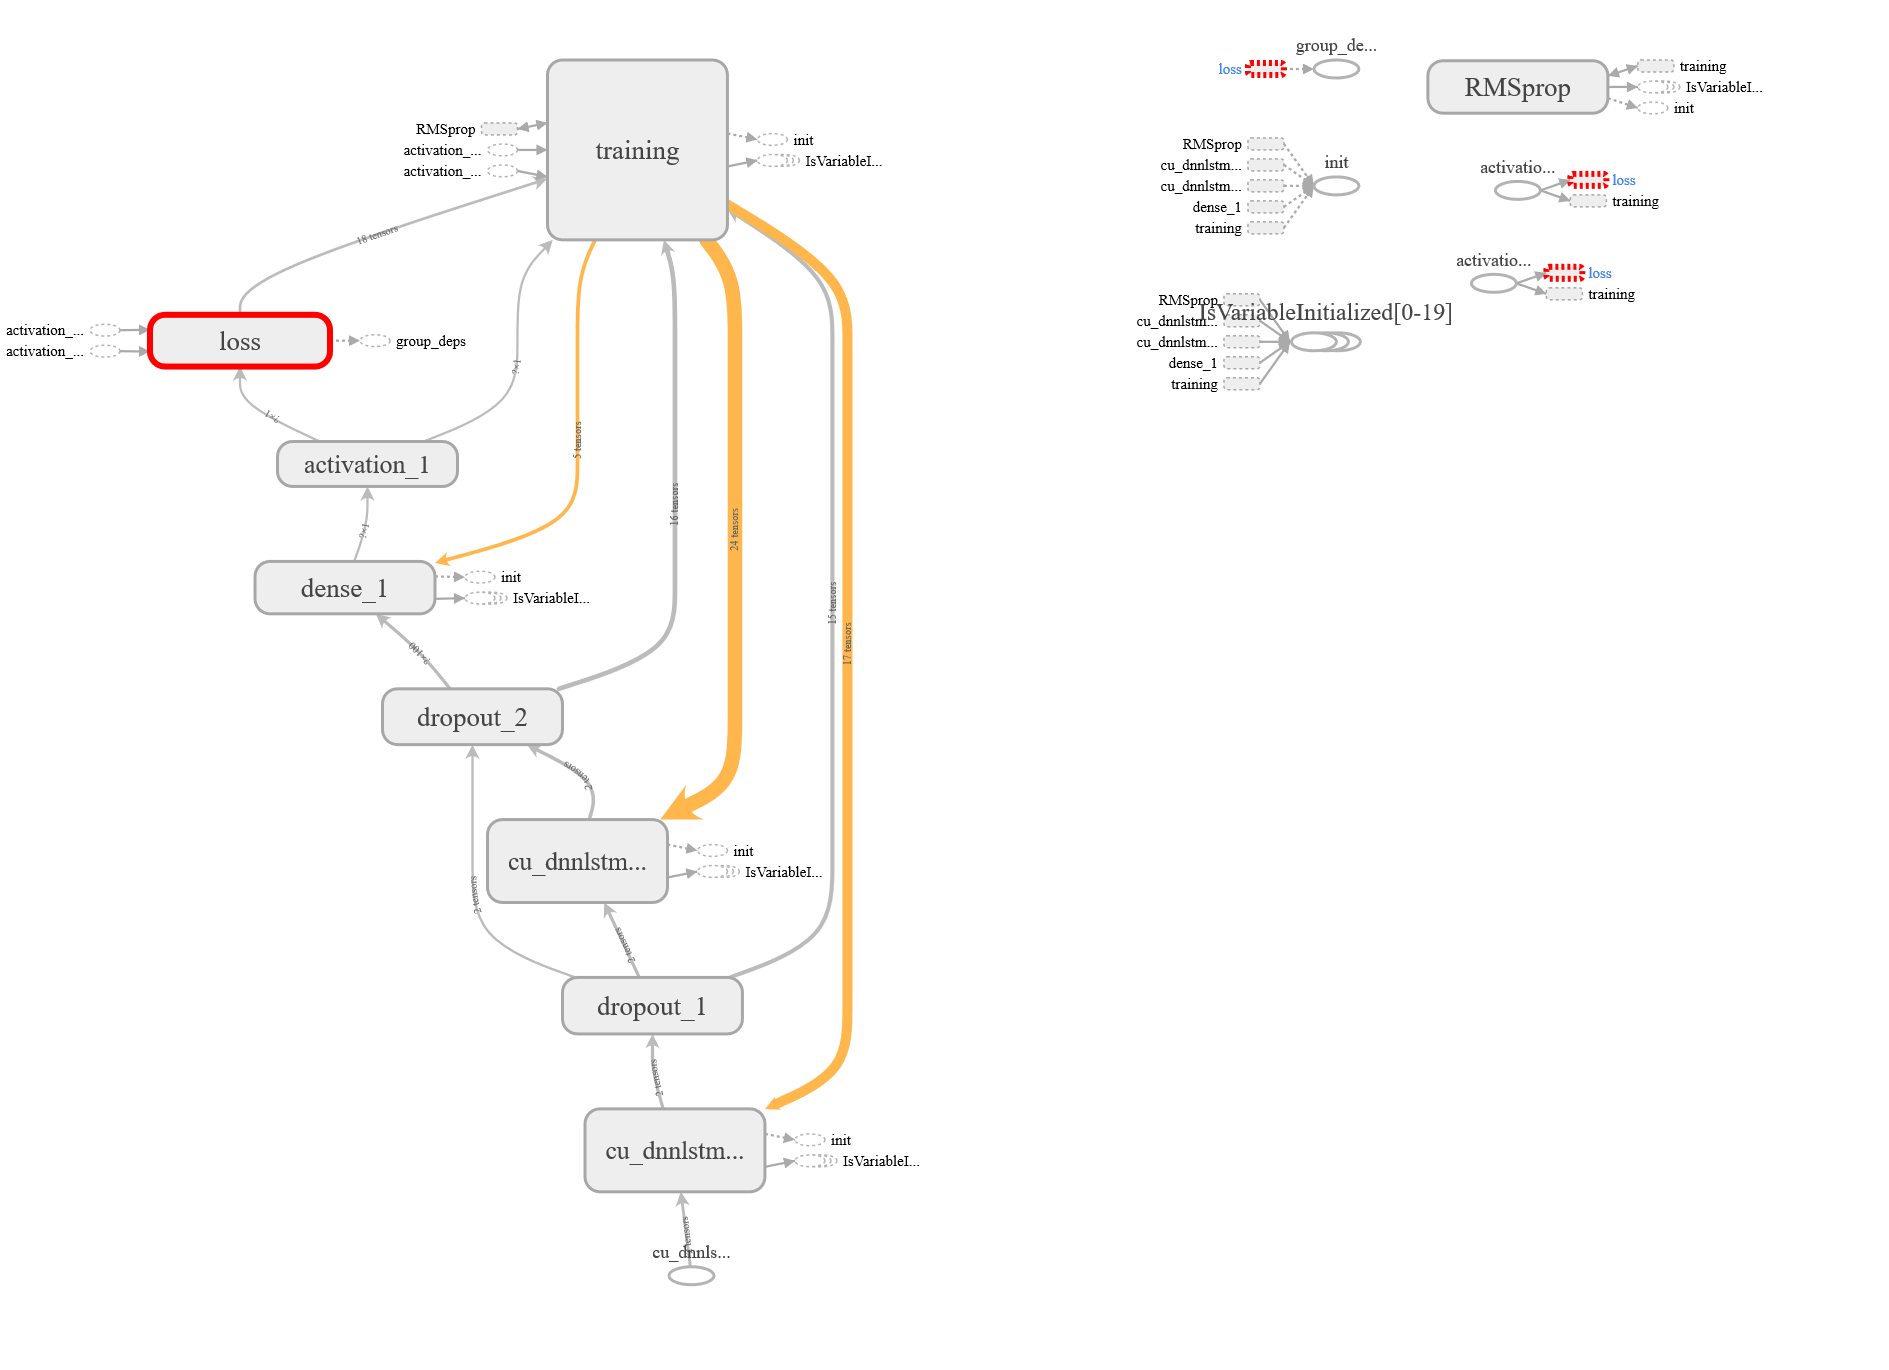
\includegraphics[width=\linewidth]{basic_architecture.png}
\caption{Basic Model Architecture}
\label{fig:basic_arch}
\end{figure}
    \subsection{Evaluating the Model}
    The trained model is run on the test set which would then collect all predictions and calculate an error score. The output shall be the calculated Root Mean Squared Error (RMSE) that gives the error in the same units as the variable itself. The data will be presented in a graph format to illustrate the improvement of the model over time.
\chapter{Results and Discussions}
\section{Experiments}

\subsection{Defining, Training and Evaluating the Model}
The following graphs and results reflect a single run unless stated otherwise.
\subsubsection{Basic Model}
In order to know the number of epochs all the models would be trained at, the basic Model with 2 layers containing 50 and 100 neurons and a Dropout of 0.2 was trained with the Early Stopping function enabled to determine when the model would no longer improve. Then it was determined that after 500 epochs the model no longer improves, and thus this would be the default number of epochs for all proceeding models.

Based on the previous research by Ruder(2016), Adam
and RMSprop are rather similar algorithms that do well in the same circumstances, however Adam slightly outperforms RMSprop, thus being the recommended optimizer. \cite{DBLP:journals/corr/Ruder16} Nonetheless both optimizers were tested using the basic model.\\


\begin{figure}[H]
    \centering
    \subfloat[train/test loss graph]{{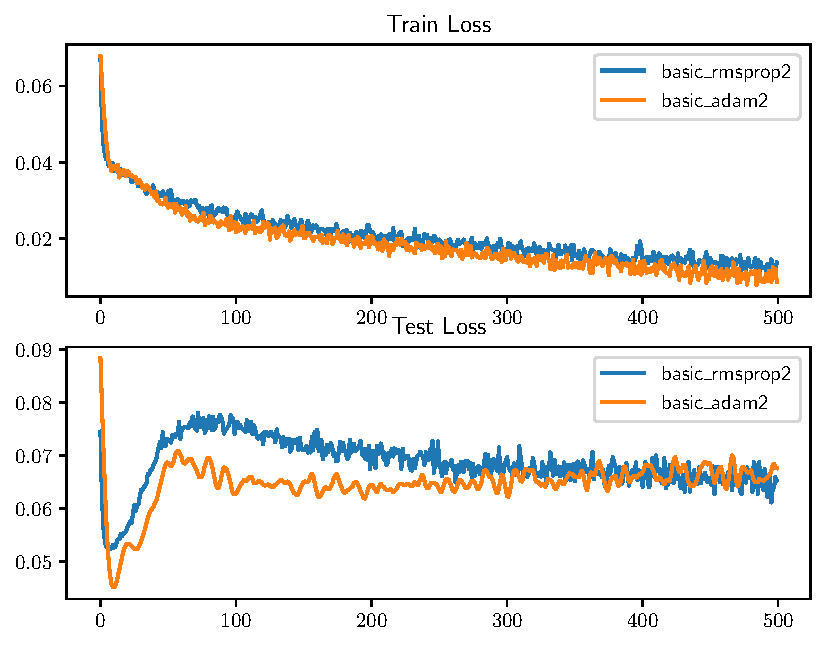
\includegraphics[width=7.5cm,height=5cm]{Data/optimizer.pdf}}}%
    \qquad
    \subfloat[prediction graph]{{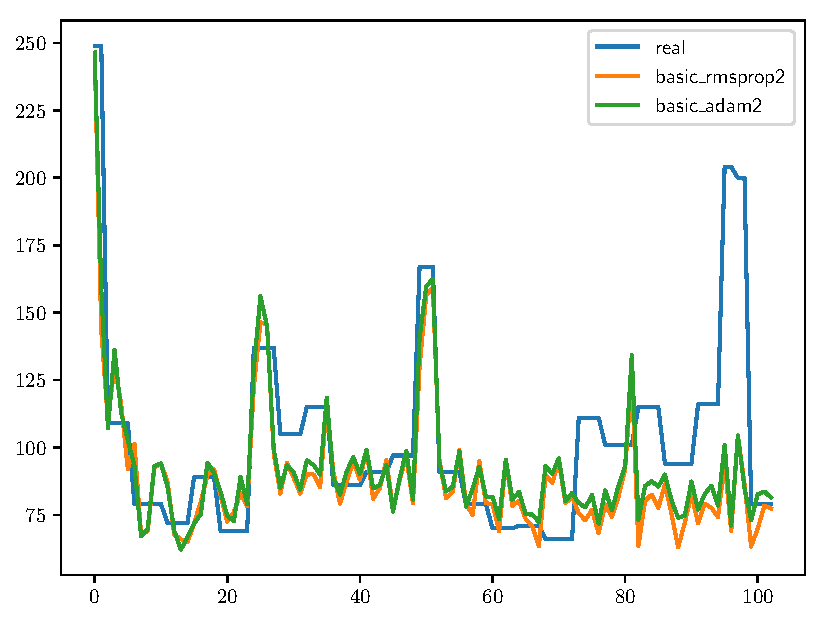
\includegraphics[width=7.5cm,height=5cm]{Data/predictions_optimizer.pdf} }}%
    \caption{Adam vs RMSprop}%
    \label{fig:basic}%
\end{figure}
\pagebreak
\begin{multicols}{2}
\centering
\begin{verbatim}
Model: basic_rmsprop2
Test RMSE: 18.68
Test  MAE: 12.33
\end{verbatim}
\begin{verbatim}
Model: basic_adam2
Test RMSE: 16.74
Test  MAE: 10.98
\end{verbatim}
\end{multicols}
From figure \ref{fig:basic} the Adam model had a lower train loss compared to the RMSprop model, but was apparently worse in the test loss. However as the RMSE was calculated in this instance, Adam showed to be a better optimizer and thus is chosen as the default for all proceeding models.\\
\subsubsection{Batch size}
The batch size was then adjusted to see whether a lower or higher batch size will improve the model. the batch size was then decreased to 20 and the RMSE decreased slightly, then it was set to 5 and the batch size had a more noticable change.\\
\begin{figure}[H]
    \centering
    \subfloat[train/test loss graph]{{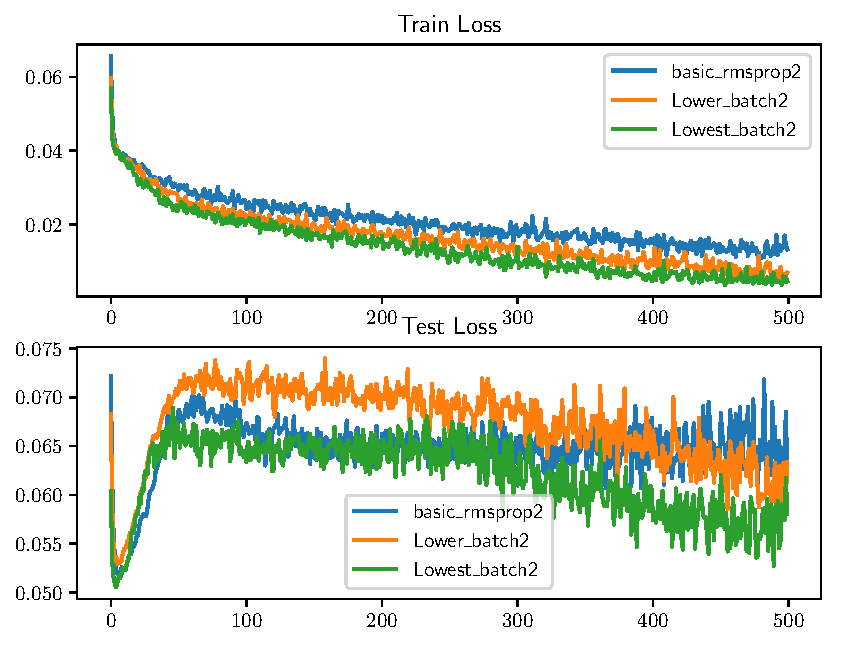
\includegraphics[width=7.5cm,height=5cm]{Data/batch_size.pdf}}}%
    \qquad
    \subfloat[prediction graph]{{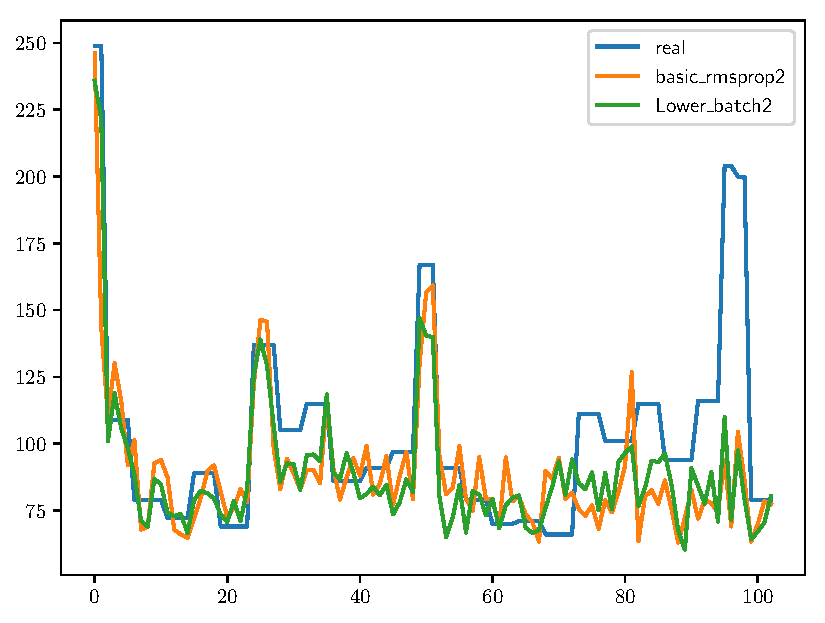
\includegraphics[width=7.5cm,height=5cm]{Data/predictions_batch_size.pdf} }}%
    \caption{Batch Size}%
    \label{fig:batch}%
\end{figure}
\begin{multicols}{3}
\centering
\begin{verbatim}
Model: basic_rmsprop2
Test RMSE: 18.68
Test  MAE: 12.33
\end{verbatim}
\begin{verbatim}
Model: Lower_batch2
Test RMSE: 13.43
Test  MAE: 10.66
\end{verbatim}
\begin{verbatim}
Model: Lowest_batch2
Test RMSE: 10.49
Test  MAE: 8.32
\end{verbatim}
\end{multicols}
\pagebreak
\subsubsection{Layers stacked}
Then more layers were added and the number of neurons was increased. Simply adding a layer created a difference in the train and test loss, the same was expected by increasing the neurons, however the train loss increased after several epochs and is an indicator of overfitting.\\
\begin{figure}[H]
    \centering
    \subfloat[train/test loss graph]{{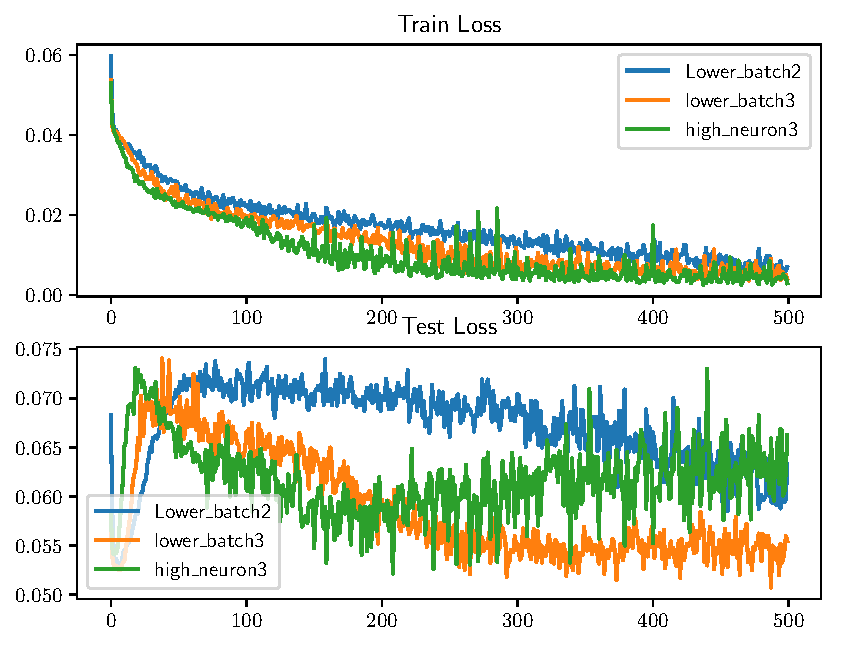
\includegraphics[width=7.5cm,height=5cm]{Data/layer_3.pdf}}}%
    \qquad
    \subfloat[prediction graph]{{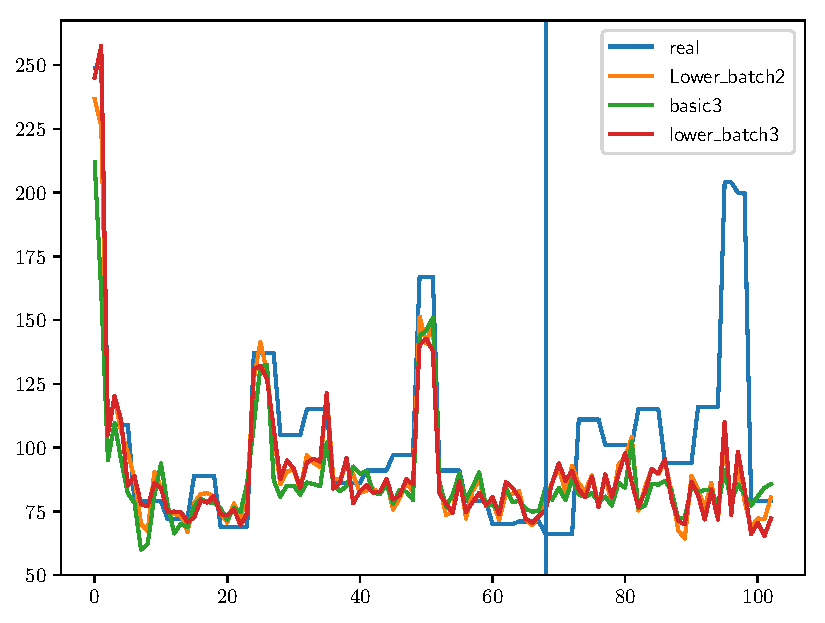
\includegraphics[width=7.5cm,height=5cm]{Data/predictions_layer_3.pdf} }}%
    \caption{Layers and Neurons tuned}%
    \label{fig:layers}%
\end{figure}
\begin{multicols}{3}
\centering
\begin{verbatim}
Model:Lowest_batch2
Test RMSE: 10.49
Test  MAE: 8.32
\end{verbatim}
\begin{verbatim}
Model: lower_batch3
Test RMSE: 10.65
Test  MAE: 8.38
\end{verbatim}
\begin{verbatim}
Model: high_neuron3
Test RMSE: 11.43
Test  MAE: 8.94
\end{verbatim}
\end{multicols}
\subsubsection{Grid Search}
A parameter grid based on all the models with a good RMSE score was then created and then a Grid Search was performed. The grid search iterates through all possible combinations of the parameter grid to find the best model with its parameters, The best model that was found by the grid search, which had 3 layers with 250, 300, 200 neurons with a batch size of 5, was then tested and its score is one of the best performing amongst other LSTM models\\
\begin{figure}[H]
    \centering
    \subfloat[train/test loss graph]{{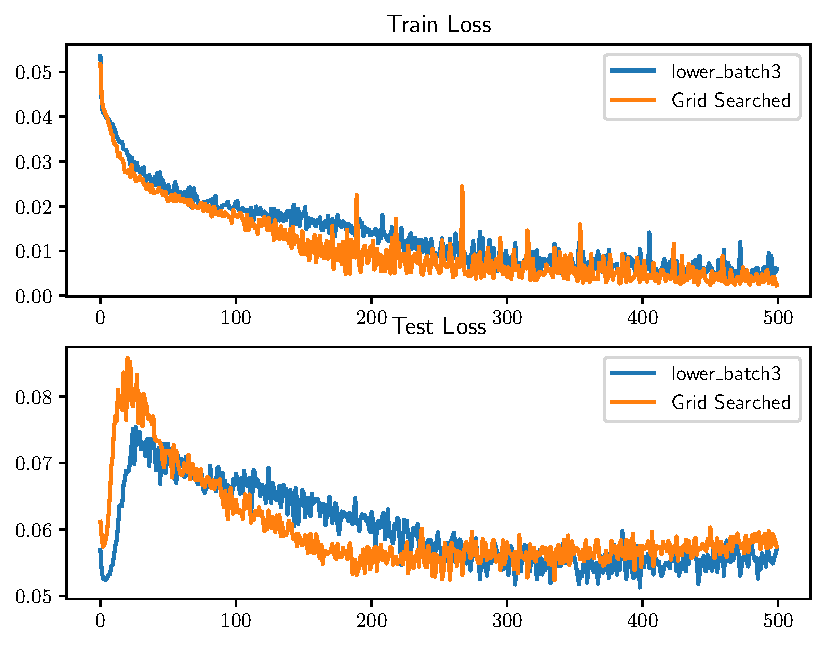
\includegraphics[width=7.5cm,height=5cm]{Data/grid_search.pdf}}}%
    \qquad
    \subfloat[prediction graph]{{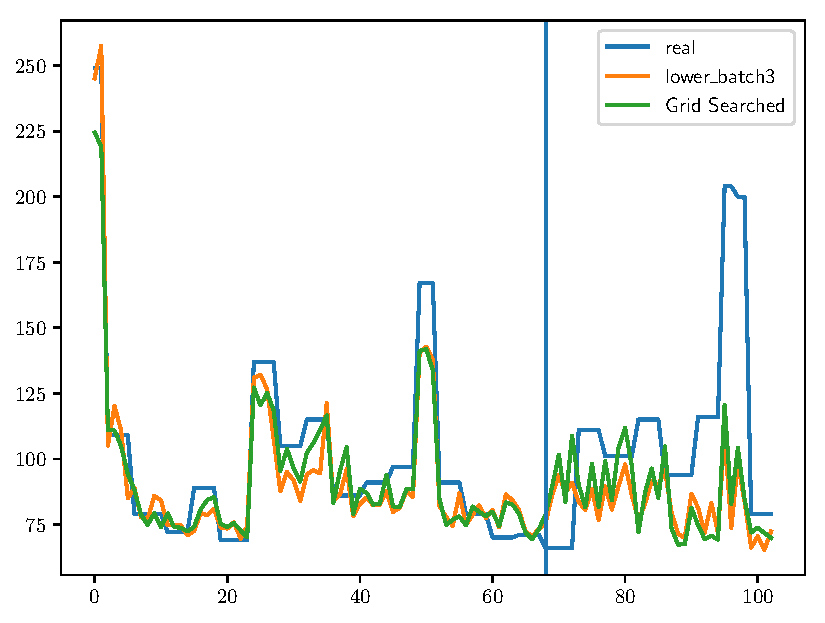
\includegraphics[width=7.5cm,height=5cm]{Data/predictions_grid_search.pdf} }}%
    \caption{Grid Search}%
    \label{fig:grid}%
\end{figure}
\begin{multicols}{2}
\centering
\begin{verbatim}
Model: lower_batch3
Test RMSE: 10.65
Test  MAE: 8.38
\end{verbatim}
\begin{verbatim}
Model: Grid Searched
Test RMSE: 8.56
Test  MAE: 7.04
\end{verbatim}
\end{multicols}
\subsubsection{Feed Forward Deep Neural Network}
Although outside the scope of the study, a basic Feed Forward Deep Neural Network (FFDNN) also known as a Multilayer Perceptron (MLP) was created to show the effect of a simpler model on a small dataset. This model averaged a 5.75 RMSE and is consistently more accurate than LSTM models. \\
\begin{figure}[H]
    \centering
    \subfloat[train/test loss graph]{{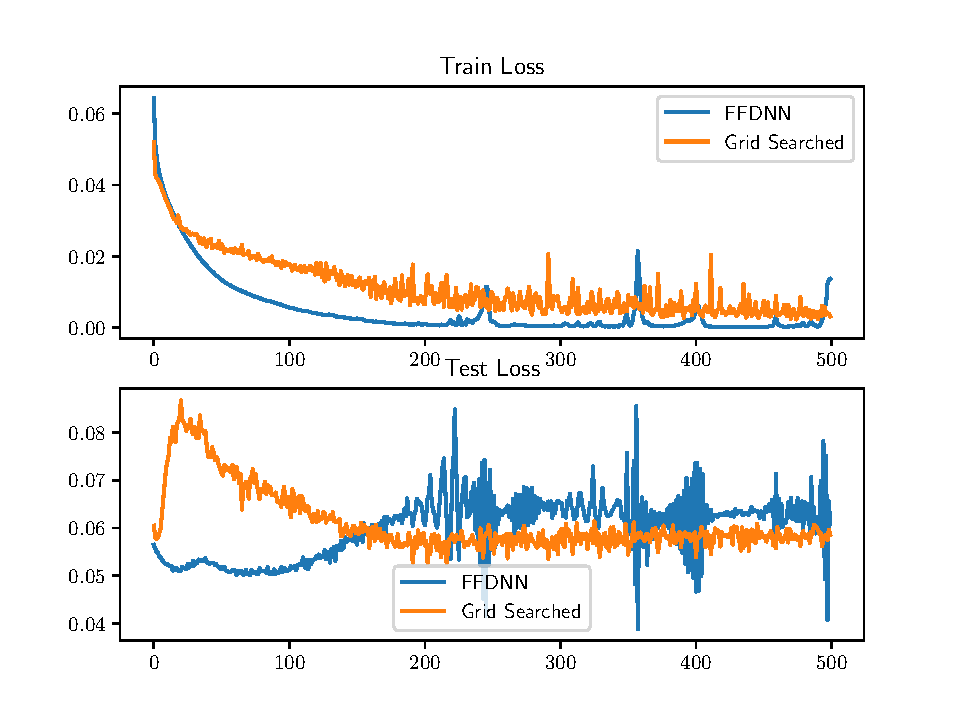
\includegraphics[width=7.5cm,height=5cm]{Data/ffdnn.pdf}}}%
    \qquad
    \subfloat[prediction graph]{{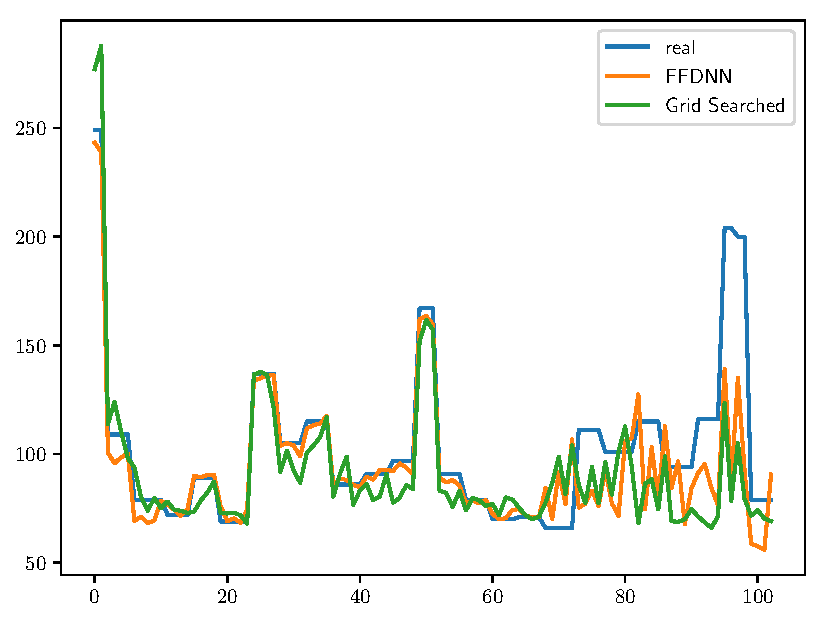
\includegraphics[width=7.5cm,height=5cm]{Data/predictions_ffdnn.pdf}}}%
    \caption{Multilayer Perceptron}%
    \label{fig:mlp}%
\end{figure}
\begin{multicols}{2}
\centering
\begin{verbatim}
Model: Grid Searched
Test RMSE: 8.56
Test  MAE: 7.04
\end{verbatim}
\begin{verbatim}
Model: FFDNN
Test RMSE: 5.88
Test  MAE: 3.92
\end{verbatim}
\end{multicols}
\section{Results}
Out of 22 models with different parameters which were trained and tested, 7 essential models were handpicked, and these models were trained and tested 100 times. The accuracy of the 7 models along with the grid searched model was gauged through an accompanying feed forward neural network on each run. All previous graph's data in a single run were collated into as single graph in figure \ref{fig:all_graphs}. While the RMSE, MAE, and range values of the models, grid search, and FFDNN were recorded and averaged for 100 runs. The parameters of the models are shown in table \ref{table:params} while the multiple values of the models' RMSE and MAE within 100 runs are shown in table \ref{table:results}\\
\begin{figure}[H]
    \centering
    \subfloat[train/test loss graph]{{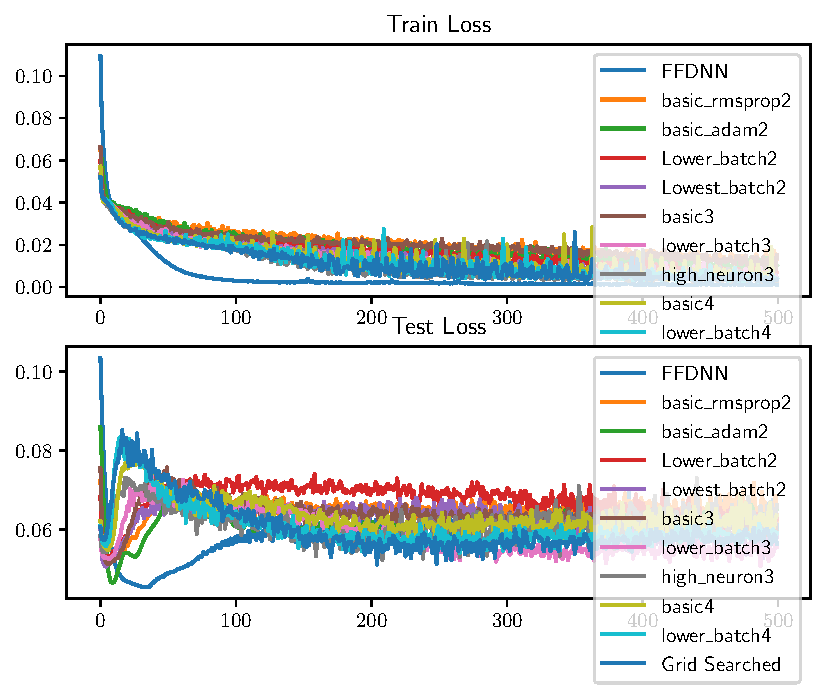
\includegraphics[width=7.5cm,height=5cm]{Data/all_models.pdf}}}%
    \qquad
    \subfloat[prediction graph]{{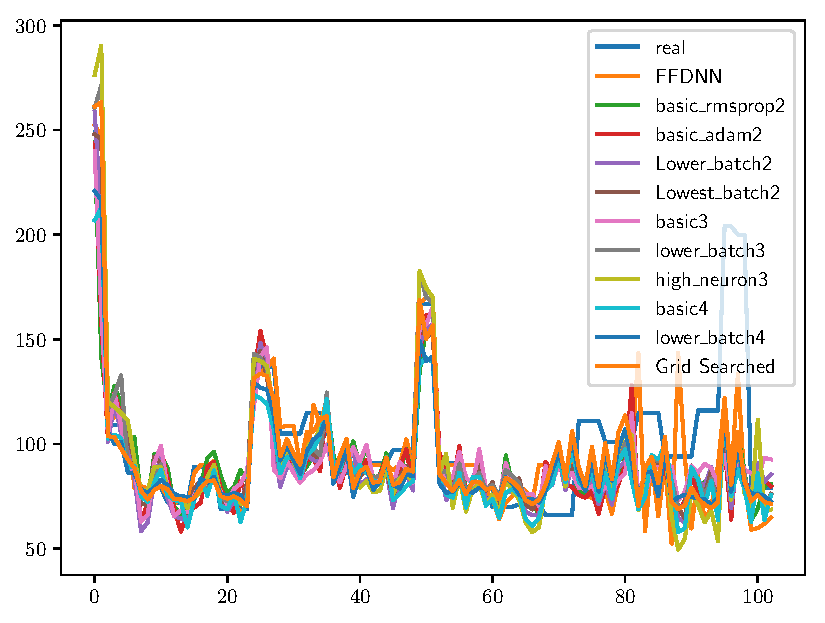
\includegraphics[width=7.5cm,height=5cm]{Data/predictions_all_models.pdf} }}%
    \caption{Multilayer Perceptron}%
    \label{fig:all_graphs}%
\end{figure}
\begin{table}[H]
\centering
\begin{threeparttable}
\begin{tabular}{ |p{2cm}||p{2.5cm}|p{1.5cm}|p{1.5cm}| p{2.5cm} | p{1.5cm}| p{1.5cm} |   }
 \hline
 \multicolumn{7}{|c|}{Parameters} \\
 \hline
Models & Number of LSTM Layers & Dropout & Dense & Optimization & Epochs & Batch Size\\
 \hline
 Basic2 & 2 (50, 100) & 0.2 & 1 (1) & rmsprop & 500 & 50\\
 \hline
 Basic ADAM2 & 2 (50, 100) & 0.2 & 1 (1) & adam & 500 & 50\\
 \hline
 Lower Batch3 & 3 (50, 100, 100) & 0.2 & 1 (1) & adam & 500 & 20\\
 \hline
 Lowest Batch3 & 3 (50, 100, 100) & 0.2 & 1 (1) & adam & 500 & 5\\
 \hline
 Basic3 & 3 (150, 250, 200) & 0.2 & 1 (1) & adam & 500 & 10\\
 \hline
Higher Neurons3 & 3 (150, 300, 200) & 0.2 & 1 (1) & adam & 500 & 5\\
 \hline
 Basic4 & 4 (150, 300, 200, 450) & 0.2 & 1 (1) & adam & 500 & 20\\
 \hline
 Lower Batch4 & 4 (150, 300, 200, 450) & 0.2 & 1 (1) & adam & 500 & 5\\
 \hline
 Grid Search3 & 3 (250, 200, 300) & 0.2 & 1 (1) & adam & 500 & 5\\
  \hline
 FFDNN & N/A & N/A & 3 (12, 8, 1) & adam & 500 & 2\\
 \hline
\end{tabular}
\begin{tablenotes}
      \small
      \item parenthesis indicates number of neurons of each layer respectively
    \end{tablenotes}
\end{threeparttable}
\caption{Parameters}
\label{table:params}
\end{table}
\begin{table}[H]
\centering
\begin{tabular}{|l|l|l|l|l|}
\toprule
Model & Ave RMSE & Range & Ave MAE & Range \\
\hline
basic\_rmsprop2  & 18.99 & 17.11-20.49 & 12.52 & 11.7-13.48 \\
\hline
basic\_adam2  & 16.71 & 15.49-18.23 & 11.41 & 10.63-12.20 \\
\hline
lower\_batch2 & 13.33 & 10.93-15.42 & 1032 & 8.48-11.69  \\
\hline
lowest\_batch2 & 11.06 & 9.21-14.85 & 8.88 & 7.51-11.57 \\
\hline
basic3 & 18.06 & 15.56-21.06 & 12.58 & 11.55-14.20 \\
\hline
lower\_batch3 & 11.15 & 9.21-15.32 & 8.57 & 7.12-11.30 \\
\hline
high\_neuron3 & 10.92 & 8.00-14.86 & 8.60 & 6.63-11.25 \\
\hline
basic4 & 13.04 & 10.04-19.31 & 10.14 & 8.27-16.54 \\
\hline
lower\_batch4 & 10.17 & 8.27-16.54 & 7.97 & 6.39-11.08 \\
\hline
Grid Searched & 10.25 & 8.08-16.23 & 7.83 & 6.17-10.76 \\
\hline
FFDNN & 5.75 & 2.55-13.34 & 4.43 & 1.85-9.76 \\
\bottomrule
\end{tabular}
\caption{Tabulated error scores}
\label{table:results}
\end{table}

\section{Discussion}
    Looking at table \ref{table:results} some initial results like the lowest\_batch2 against high\_neuron3 had a different outcome after multiple runs, as it seemed that lowest\_batch2 was better but it actually was a result of high\_neuron3 overfitting in that specific instance. With high\_neuron3 being better it seems that a higher number of layers coupled with an increase in neurons actually has a noticeable effect on the RMSE. The grid searched model also presents this effect with all its layers consisting of 200 and more neurons. Then the effect of batch size is seen in all basic to lower batch models, a large decrease in batch size also has a large decrease in the RMSE, this is a side effect of the high number of iterations of fitting, before finishing a single epoch. A batch size of 50 would have 2 steps before finishing an epoch, while a batch size of 5 would have 14 steps, thus increasing the learning capabilities of the model. Then with these effects in mind, an experiment with 4 layers LSTM was conducted, and it produced the best model amongst LSTM models. With the caveat that it has the longest training time: \begin{verbatim}
Time for high_neuron3:0:00:32.737798
Time for lower_batch4:0:01:26.715916
Time for Grid Searched:0:01:05.732816
    \end{verbatim}
    This ~50\% to ~300\% increase in training time makes it impractical to grid search, taking days to weeks to find the best model.
    In the end the two best performing models are Lower Batch4 and Grid Search3. Giving the impression that a lower batch size coupled with high neurons and number of layers would result in a better score. Based on the results, it shows that RNNs can accurately predict hospitalization rate, as they are on average 10 cases off the true value, with the true value being on average 103.
\chapter{Conclusions and Recommendations}
\section{Conclusions}
Recurrent Neural Networks work by analyzing current and previous inputs in calculating their prediction. Unlike neural networks such as Feed Forward wherein information runs in only one direction, information in RNNs runs in a loop; for every succeeding input, the information of each input is stored and taken into account in the calculation of the networks' prediction. In short, the RNNs remember previous information in their calculations. Although normal RNNs suffer from the vanishing gradient problem, wherein it struggles to remember inputs far away in the sequence, modified RNNs such as Long Short-Term Memory and Gated Recurrent Unit are used to deal with this problem, with the former being used for this study. It can be inferred that the 10\% error achieved is due to the structure of the LSTMs enabling it to remember long-term inputs despite a large number of data and epochs. 

Pollutants and their concentration levels can be measured by dedicated air pollution monitoring analyzers and sensors. In gathering the pollution data, the DENR used state-of-the-art air monitoring analyzers; namely, Open-Path Dedicated Outdoor Air Systems (DOAS) and Continuous Ambient Monitoring Stations (CAMS). These air monitoring analyzers measure pollutants such as carbon dioxide (CO2) and ozone (O3) which are used in this study. Air Quality Indices are also useful to gauge the concentration levels of pollutants, which were used by DENR to know if said levels of pollutants were dangerous or not.

Predicting the number of hospitalization cases is fairly easy outside of being accurate. The pollution data is correlated with the hospitalization cases data and is subsequently used as the dataset for the RNN models. The RNN models' parameters are tuned with the desired values of the proponents and are run for training and testing. These models then output their predicted number of hospitalization cases. Inside of being accurate, however, was the main frustration of this research. While grid searching was used to get the best parameters out of a specified range of values, it took a long time to train and compare multiple models. In the end, it all boiled down to trial and error, tuning each parameter of the model until it scores a lower error value resulting in a close to the real value of hospitalizations cases found in the gathered data. 

Determining the accuracy of the models' prediction of hospitalization cases can be measured using Root-Mean-Square Error (RMSE). The RMSE outputs the percentage number on how much the predicted numbers of the models deviated from the real number of hospitalization cases found in gathered data. Since the RMSE is expressed in the same units as the output value, it can be compared to the average value of the target. A 10.25 score compared to an average value of 103 can be likened to a $\approx$10\% deviation or $\approx$90\% accuracy. Although a model outside the scope of the study, the FFDNN, had better accuracy than the LSTM, this could be a good subject of study.

Results of the accuracy of the most efficient models Lower Batch4 and Grid Search3 indicates a correlation between air quality and hospitalization cases. For further insight, each pollutant level from a different station, or group of stations yielded the following correlation levels with Target.

\begin{table}
\begin{center}
\begin{table}
    \centering
    \begin{tabular}{|l|l|l|l|l|}
\toprule
Station    & pm10  & so2   & no2   & o3    \\
\hline
1st  & -0.001178 & 0.064983   & -0.157946    & -0.175356   \\
\hline
2nd  & -0.183510 & 0.047820 & -0.266901   & -0.180209   \\
\hline
3rd  & -0.014404 & 0.072528  & -0.001774 & -0.043407  \\
\hline
4th & -0.158424 & 0.025202 & -0.171389  & -0.076618    \\
\bottomrule
\end{tabular}
    \caption{Correlation }
    \label{table:correl}
\end{table}

\end{center}
\caption{Correlation Results}
\label{table:correlation}
\end{table}

Correlation is measured from -1 to 0 to 1, with -1 signifying an inverse correlation between pollutant levels and Target, 1 for a positive correlation, and 0 for no correlation at all.

Among all pollutants, Sulfur Dioxide seems to be the highest possible cause of lung-related hospitalizations cases due to having positive correlation for all stations, while the other pollutants, having negative correlation, may not necessarily lead to high number of hospitalizations cases even having high levels. At the very least, this data signifies that poor air quality does have an effect on the number of lung-related hospitalizations; its severity dependent on the kind of pollutant/s involved.


\section{Recommendations}
For future studies related to this research, it is recommended to utilize a larger dataset with shorter time intervals, e.g. daily data. The larger amount of data could possibly help the model detect more trends and increase the accuracy. 
In addition, based on the results of this research the FFDNN are warranted to be researched on due to the fact it performed better than the best RNN models. A study on FFDNN accuracy levels similar to this research is recommended.
For future proponents who will be conducting research related to hospitalization cases, it's recommended to use Davao Doctors Hospital as a source of data due to having a database system of their own and an extensive number of cases.
    \bibliographystyle{acm}
    \bibliography{ref}
\end{document}
